%%%%%%%%%%%%%%%%%%%%%%%%%%%%%%
%
% $Autor: Wings $
% $Datum: 2019-12-09 11:50:02Z $
% $Pfad: komponenten/Bilderkennung/Produktspezifikation/CorelTPU/TPU/Allgemein/tikzdefs.tex $
% $Version: 1766 $
%
%
%%%%%%%%%%%%%%%%%%%%%%%%%%%%%%


% Definition für tikz

\usepackage{pgfplots}
\usepackage{pgf,tikz}
\usepackage{mathrsfs}
\usepackage{circuitikz}
\usepackage{tikz}
\usetikzlibrary{shapes,shapes.symbols,shapes.misc, shapes.multipart, shapes.geometric,arrows,angles,quotes,babel,positioning,calc,math,matrix,backgrounds}
\usetikzlibrary{positioning,fadings,through}
\usetikzlibrary{math}


\usepackage{tikz-3dplot}

\definecolor{ArduinoColor}{rgb}{0.1,0.5,0.6}
\definecolor{BlackGreen}{rgb}{0.5, 0.68,0.375}
\definecolor{Or}{rgb}{0.945, 0.768,0.0588}
\definecolor{Cyann}{rgb}{0.1,0.9,0.9}
\definecolor{DarkOrange}{rgb}{0.89, 0.4,0.09}
\definecolor{Gold}{rgb}{0.733, 0.647, 0.239}
\definecolor{Purple}{rgb}{0.416, 0, 0.761}


\tikzset{
  input2/.style={ % requires library shapes.geometric
    draw,
    trapezium,
    trapezium left angle=60,
    trapezium right angle=120,
  },
  process rectangle outer width/.initial=0.15cm,
  predefined process/.style={
    rectangle,
    draw,
    append after command={
      \pgfextra{
        \draw [fill=blue!20]
        ($(\tikzlastnode.north west)-(0,0.5\pgflinewidth)$)--
        ($(\tikzlastnode.north west)-(\pgfkeysvalueof{/tikz/process rectangle outer width},0.5\pgflinewidth)$)--
        ($(\tikzlastnode.south west)+(-\pgfkeysvalueof{/tikz/process rectangle outer width},+0.5\pgflinewidth)$)--
        ($(\tikzlastnode.south west)+(0,0.5\pgflinewidth)$);
        \draw [fill=blue!20]
        ($(\tikzlastnode.north east)-(0,0.5\pgflinewidth)$)--
        ($(\tikzlastnode.north east)+(\pgfkeysvalueof{/tikz/process rectangle outer width},-0.5\pgflinewidth)$)--
        ($(\tikzlastnode.south east)+(\pgfkeysvalueof{/tikz/process rectangle outer width},0.5\pgflinewidth)$)--
        ($(\tikzlastnode.south east)+(0,0.5\pgflinewidth)$);
      }  
    },
    text width=#1,
    align=center, fill=blue!20,  minimum height=4em
  },
  predefined process/.default=20mm,
  data1/.style={
    trapezium, 
    trapezium left angle=70, 
    trapezium right angle=110, 
    text width=1.5cm, 
    inner ysep=17pt,
    align=center, 
    line width=2pt,
    fill=blue!20
  },      
}


%Kabinettprojektion von 3D auf 2D
%
% Eingabe
% x,y,z
%
% Ausgabe
% x- oder y-Wert des Punkts
\newcommand{\Proj}[3]{({#1-#3*0.5*cos(30)},{#2-#3*0.5*sin(30)})}
\tikzset{declare function={ProjX(\x,\y,\z)=\x-\z*0.5*cos(30);}}
\tikzset{declare function={ProjY(\x,\y,\z)=\y-\z*0.5*sin(30);}}

%Rotation um die x-Achse 
%
% Eingabe
% x,y,z,alpha
%
% Ausgabe
% 
% x-, y- oder z-Wert des Punkts
\tikzset{declare function={RotXx(\x,\y,\z,\a)=\x;}}
\tikzset{declare function={RotXy(\x,\y,\z,\a)=\y*cos(\a)-\z*sin(\a);}}
\tikzset{declare function={RotXz(\x,\y,\z,\a)=\y*sin(\a)+\z*cos(\a);}}


%Rotation um die y-Achse 
%
% Eingabe
% x,y,z,alpha
%
% Ausgabe
% 
% x-, y- oder z-Wert des Punkts
\tikzset{declare function={RotYx(\x,\y,\z,\a)=\x*cos(\a)-\z*sin(\a);}}
\tikzset{declare function={RotYy(\x,\y,\z,\a)=\y;}}
\tikzset{declare function={RotYz(\x,\y,\z,\a)=\x*sin(\a)+\z*cos(\a);}}



%Rotation um die z-Achse 
%
% Eingabe
% x,y,z,alpha
%
% Ausgabe
% 
% x-, y- oder z-Wert des Punkts
\tikzset{declare function={RotZx(\x,\y,\z,\a)=\x*cos(\a)-\y*sin(\a);}}
\tikzset{declare function={RotZy(\x,\y,\z,\a)=\x*sin(\a)+\y*cos(\a);}}
\tikzset{declare function={RotZz(\x,\y,\z,\a)=\z;}}


%Rotation um die x-Achse 
%
% Eingabe
% x,y,z,alpha
%
% Ausgabe
% Punkt {x}{y}{z}
\newcommand{\RotXx}[4]{#1}%
\newcommand{\RotXy}[4]{(cos(#4)*#2-sin(#4)*#3)}
\newcommand{\RotXz}[4]{(sin(#4)*#2+cos(#4)*#3)}%


\tikzset{declare function={bellshape(\x,\mu,\sigma)=exp(-(\x-\mu)^2/(2*\sigma^2));}}


%Rotation um die x-Achse mit Projektion
%
% Eingabe
% x,y,z,alpha
%
% Ausgabe
% Punkt ({x}, {y})
\newcommand{\RotXP}[4]%
{(%
{#1-(sin(#4)*#2+cos(#4)*#3)*0.5*cos(30)},%
{cos(#4)*#2-sin(#4)*#3-(sin(#4)*#2+cos(#4)*#3)*0.5*sin(30)})%
}

%Rotation um die y-Achse mit Projektion
%
% Eingabe
% x,y,z,alpha
%
% Ausgabe
% Punkt ({x}, {y})
\newcommand{\RotYP}[4]%
{(%
{cos(#4)*#1+sin(#4)*#3-(-sin(#4)*#1+cos(#4)*#3)*0.5*cos(30)},%
{#2-(-sin(#4)*#1+cos(#4)*#3)*0.5*sin(30)}%
)}


%Rotation um die z-Achse mit Projektion
%
% Eingabe
% x,y,z,alpha
%
% Ausgabe
% Punkt ({x}, {y})
\newcommand{\RotZP}[4]%
{({cos(#4)*#1-sin(#4)*#2-#3*0.5*cos(30)},{sin(#4)*#1+cos(#4)*#2-#3*0.5*sin(30)})}


% Parameter
% #1: Skalierung
% #2: Winkel; 0..179
\newcommand{\HermiteSymPSP}[2]{%
  \pgfmathsetmacro{\RADIUS}{6}
  
  \begin{scope}[scale=#1]
    
    % angle 
    \begin{scope}[shift={(\RADIUS,0cm)}]
      \draw[fill=green!30] (0,0) -- (180:0.25*\RADIUS) arc (180:#2:0.25*\RADIUS);
      \draw ({0.5*(180+#2)}:{0.175*\RADIUS}) node {$\beta$};
      \draw ({0.5*(#2)}:{0.175*\RADIUS}) node {$\alpha$}; %$\pi-\alpha$
    \end{scope}
    
    \coordinate[label=left:$P_0$]  (P0) at (0,0);
    \coordinate  (t0) at (0.25*\RADIUS,0);
    \coordinate[label=below:$S$]  (S) at (\RADIUS,0);
    \coordinate  (s0) at (1.3*\RADIUS,0);
    \coordinate[label=left:$P_1$] (P1) at ({\RADIUS+\RADIUS*cos(#2)},{\RADIUS*sin(#2)});
    
    \draw [black,line width=0.5pt,domain=0:#2,->] plot ({\RADIUS+0.25*\RADIUS*cos(\x)}, {0+0.25*\RADIUS*sin(\x)});
    
    \draw [line width=1.5pt] (P0) -- (S) --(P1);
    \draw [line width=0.2pt,dotted] (S) --(s0);
    \node (P00) at (P0) {$\bullet$};
    \node (P11) at (P1) {$\bullet$};
  \end{scope}
}


% Parameter
% #1: Skalierung
% #2: Winkel; 0..179
\newcommand{\HermiteSym}[2]{%
   \pgfmathsetmacro{\RADIUS}{6}
  
   \begin{scope}[scale=#1]

     % angle 
     \begin{scope}[shift={(\RADIUS,0cm)}]
       \draw[fill=green!30] (0,0) -- (180:0.25*\RADIUS) arc (180:#2:0.25*\RADIUS);
       \draw ({0.5*(180+#2)}:{0.175*\RADIUS}) node {$\beta$};
       \draw ({0.5*(#2)}:{0.175*\RADIUS}) node {$\alpha$}; %$\pi-\alpha$
     \end{scope}

     \coordinate[label=left:$P_0$]  (P0) at (0,0);
     \coordinate  (t0) at (0.25*\RADIUS,0);
     \coordinate[label=below:$S$]  (S) at (\RADIUS,0);
     \coordinate  (s0) at (1.3*\RADIUS,0);
     \coordinate[label=left:$P_1$] (P1) at ({\RADIUS+\RADIUS*cos(#2)},{\RADIUS*sin(#2)});
     \coordinate (t1) at ({\RADIUS+ 1.25*\RADIUS*cos(#2)},{1.25*\RADIUS*sin(#2)});
  
     \coordinate[label=below:$\vec{t}_0$](T0) at ($ (P0)!.5!(t0) $);
     \coordinate[label=right:$\vec{t}_1$](T1) at ($ (P1)!.5!(t1) $);

     \draw [black,line width=0.5pt,domain=0:#2,->] plot ({\RADIUS+0.25*\RADIUS*cos(\x)}, {0+0.25*\RADIUS*sin(\x)});

     \draw [line width=1.5pt] (P0) -- (S) --(P1);
     \draw [line width=2pt,->,color=red] (P0) -- (t0);
     \draw [line width=2pt,->,color=red] (P1) -- (t1);
     \draw [line width=0.2pt,dotted] (S) --(s0);
     \node (P00) at (P0) {$\bullet$};
     \node (P11) at (P1) {$\bullet$};
  \end{scope}
}


% Parameter
% #1: Skalierung
% #2: Winkel; 0..-179
\newcommand{\HermiteSymNeg}[2]{%
  \pgfmathsetmacro{\RADIUS}{6}
  
  \begin{scope}[scale=#1]
    
    % angle 
    \begin{scope}[shift={(\RADIUS,0cm)}]
      \draw[fill=green!30] (0,0) -- (-180:0.25*\RADIUS) arc (-180:#2:0.25*\RADIUS);
      \draw ({0.5*(-180+#2)}:{0.175*\RADIUS}) node {$\beta$};
      \draw ({0.5*(#2)}:{0.175*\RADIUS}) node {$\alpha$}; %$\pi-\alpha$
    \end{scope}
    
    \coordinate[label=left:$P_0$]  (P0) at (0,0);
    \coordinate  (t0) at (0.25*\RADIUS,0);
    \coordinate[label=above:$S$]  (S) at (\RADIUS,0);
    \coordinate  (s0) at (1.3*\RADIUS,0);
    \coordinate[label=left:$P_1$] (P1) at ({\RADIUS+\RADIUS*cos(#2)},{\RADIUS*sin(#2)});
    \coordinate (t1) at ({\RADIUS+ 1.25*\RADIUS*cos(#2)},{1.25*\RADIUS*sin(#2)});
    
    \coordinate[label=below:$\vec{t}_0$](T0) at ($ (P0)!.5!(t0) $);
    \coordinate[label=right:$\vec{t}_1$](T1) at ($ (P1)!.5!(t1) $);
    
    \draw [black,line width=0.5pt,domain=0:#2,->] plot ({\RADIUS+0.25*\RADIUS*cos(\x)}, {0+0.25*\RADIUS*sin(\x)});
    
    \draw [line width=1.5pt] (P0) -- (S) --(P1);
    \draw [line width=2pt,->,color=red] (P0) -- (t0);
    \draw [line width=2pt,->,color=red] (P1) -- (t1);
    \draw [line width=0.2pt,dotted] (S) --(s0);
    \node (P00) at (P0) {$\bullet$};
    \node (P11) at (P1) {$\bullet$};
  \end{scope}
}

\tikzstyle{bigblock} = [draw, fill=blue!20, rectangle, minimum height=1.5em, minimum width=8em]
\tikzstyle{mediumblock} = [draw, fill=red!20, rectangle, minimum height=1.5em, minimum width=4em]
\tikzstyle{smallblock} = [draw, fill=red!20, rectangle, minimum height=1.5em, minimum width=1.5em]
\tikzstyle{arrow} = [->,shorten >=1pt,>=stealth',semithick]

\definecolor{LightCyan}{rgb}{0.88,1,1}
\definecolor{frenchblue}{rgb}{0.0, 0.45, 0.73}
\definecolor{greenblue}{rgb}{0.0, 0.25, 0.3}
\definecolor{darkcyan}{rgb}{0.0, 0.55, 0.55}
\definecolor{bondiblue}{rgb}{0.0, 0.58, 0.71}
\definecolor{grayleft}{rgb}{0.1, 0.1, 0.1}
\definecolor{grayright}{rgb}{0.2, 0.2, 0.2}
\definecolor{graycircle}{rgb}{0.3, 0.3, 0.3}
\definecolor{graylight}{rgb}{0.8, 0.8, 0.8}
\definecolor{greenenglish}{rgb}{0.0, 0.5, 0.0}
\definecolor{darkpastelgreen}{rgb}{0.01, 0.75, 0.24}
\definecolor{copper}{rgb}{0.72, 0.45, 0.2}
\definecolor{greenyellow}{rgb}{0.68, 1.0, 0.18}
\definecolor{fuchsia}{rgb}{1.0, 0.0, 1.0}
\definecolor{silver}{rgb}{0.75, 0.75, 0.75}
\definecolor{deepskyblue}{rgb}{0.0, 0.75, 1.0}

% Beispiele
%
%\begin{center}
%  \begin{tikzpicture}
%  \HermiteSym{1}{120}
%  \end{tikzpicture}
%\end{center}
%
%\begin{center}
%  \begin{tikzpicture}
%  \HermiteSym{1}{70}
%  \end{tikzpicture}
%\end{center}
%
%\begin{center}
%  \begin{tikzpicture}
%  \HermiteSym{1}{20}
%  \end{tikzpicture}
%\end{center}
%
%\begin{center}
%  \begin{tikzpicture}
%  \HermiteSym{1}{0}
%  \end{tikzpicture}
%\end{center}
%
%
%\begin{center}
%  \begin{tikzpicture}
%  \HermiteSymNeg{1}{-20}
%  \end{tikzpicture}
%\end{center}
%
%\begin{center}
%  \begin{tikzpicture}
%  \HermiteSymNeg{1}{-70}
%  \end{tikzpicture}
%\end{center}
%
%
%\begin{center}
%  \begin{tikzpicture}
%  \HermiteSymNeg{1}{-120}
%  \end{tikzpicture}
%\end{center}
%

%tikz-Kommandos

% Basis eines Roboters
% #1: Drehung des Systems
% #2: X-Offset des gedrehten Systems
% #3: Y-Offset des gedrehten Systems
% #4: Skalierung
\newcommand{\BASE}[4]{
  \begin{scope}[rotate=#1,scale=#4]  
    
    \draw[ultra thick, black]   ({#2-0.5},{#3-0.7}) -- ({#2+0.5},{#3-0.7});
    \draw[ultra thick, black]   ({#2-0.3},{#3-0.7}) -- ({#2-0.5},{#3-0.9});    
    \draw[ultra thick, black]   ({#2-0.1},{#3-0.7}) -- ({#2-0.3},{#3-0.9});    
    \draw[ultra thick, black]   ({#2+0.1},{#3-0.7}) -- ({#2-0.1},{#3-0.9});    
    \draw[ultra thick, black]   ({#2+0.3},{#3-0.7}) -- ({#2+0.1},{#3-0.9});    
    \draw[ultra thick, black]   ({#2+0.5},{#3-0.7}) -- ({#2+0.3},{#3-0.9});    
    
    \draw[thick, fill=blue!20]   ({#2-0.25},{#3-0.7}) -- ({#2+0.25},{#3-0.7}) -- ({#2},{#3}) -- ({#2-0.25},{#3-0.7});
    \draw[black, thick, fill=black]  (#2,#3) ellipse (0.1 and 0.1);
  \end{scope}
}%  


% Drehgelenk eines Roboters
% #1: Drehung des Gelenks
% #2: X-Offset des Systems
% #3: Y-Offset des Systems
% #4: Skalierung
\newcommand{\LINK}[4]{
  \begin{scope}[scale=#4]
    \draw[green, thick, fill=green!20]  ({#2+0.0},{#3+0.0}) ellipse (0.2 and 0.2);
    \draw[green, thick, fill=green!20]  ({#2+2.0*cos(#1)},{#3+2.0*sin(#1)}) ellipse (0.2 and 0.2);
    \draw[green!20, thick, fill=green!20]
    ({#2+0+0.2*cos(90+#1)},{#3+0+0.2*sin(90+#1)})
    --
    ({#2+2.0*cos(#1)+0.2*cos(90+#1)},{#3+2.0*sin(#1)+0.2*sin(90+#1)})
    --
    ({#2+2.0*cos(#1)+0.2*cos(-90+#1)},{#3+2.0*sin(#1)+0.2*sin(-90+#1)})
    --
    ({#2+0+0.2*cos(-90+#1)},{#3+0+0.2*sin(-90+#1)})
    --
    ({#2+0+0.2*cos(90+#1)},{#3+0+0.2*sin(90+#1)});
    \draw[green, thick]
    ({#2+0+0.2*cos(90+#1)},{#3+0+0.2*sin(90+#1)})
    --
    ({#2+2.0*cos(#1)+0.2*cos(90+#1)},{#3+2.0*sin(#1)+0.2*sin(90+#1)});
    \draw[green, thick]
    ({#2+2.0*cos(#1)+0.2*cos(-90+#1)},{#3+2.0*sin(#1)+0.2*sin(-90+#1)})
    --
    ({#2+0+0.2*cos(-90+#1)},{#3+0+0.2*sin(-90+#1)});
    \draw[black, thick, fill=blue]  ({#2+0.0},{#3+0.0}) ellipse (0.1 and 0.1);
    \draw[black, thick, fill=black]  ({#2+2*cos(#1)},{#3+2*sin(#1)}) ellipse (0.1 and 0.1);
    
  \end{scope}
}%  

% Drehgelenk eines Roboters
% #1: 1.Punkt x
% #2: 1.Punkt y
% #3: 2.Punkt x
% #4: 2.Punkt y
\newcommand{\LINKP}[4]{
  \begin{scope}
     \tikzmath{
       \Px  = #1;
       \Py  = #2;
       \Qx  = #3;
       \Qy  = #4;
       \Dx   = \Qx-\Px;
       \Dy   = \Qy-\Py;
       \Winkel = 45;
       \Pp  = \Dy*pow(\Dx,-1);
       \Winkel = atan(\Pp);
       \Laenge = pow(pow(\Dx,2)+pow(\Dy,2),0.5);
     }    
    
  
    \LINK{\Winkel}{#1}{#2}{1}
  \end{scope}
}%  

% SCARA-Roboters
% #1: Drehung des Systems
% #2: X-Offset des gedrehten Systems
% #3: Y-Offset des gedrehten Systems
% #4: Winkel des 1.Gelenks
% #5: Winkel des 2.Gelenks
% #6: Skalierung
% #7: Auswahl ungerade mit Beschriftung der Armlängen 
%           2 und 3: mit Winkel

\newcommand{\SCARA}[7]{
  \def\Rot{#1}
  \def\OffsetX{#2}
  \def\OffsetY{#1}
  \def\Alpha{#4}
  \def\Beta{#5}
  \def\Auswahl{#7}
  
  \begin{scope}[scale=#6]
    \BASE{\Rot}{\OffsetX}{\OffsetY}{1}
    \LINK{\Alpha}{\OffsetX}{\OffsetY}{1}
    \LINK{\Beta}{\OffsetX+2*cos(\Alpha)}{\OffsetY+2*sin(\Alpha)}{1}
    
    \ifthenelse{\isodd{\Auswahl}}
    {
        \node (Q1T) at (\OffsetX-0.6,\OffsetY) {$(0,0)$};
        \node (Q2T) at ({\OffsetX+1*cos(\Alpha)-0.4*sin(\Alpha)},{\OffsetY+1*sin(\Alpha)+0.4*cos(\Alpha)}) {$\ell_1$};
        \node (Q3T) at ({\OffsetX+2*cos(\Alpha)+1*cos(\Alpha+\Beta)+0.2*sin(\Alpha+\Beta)},{\OffsetY+2*sin(\Alpha)+1*sin(\Alpha+\Beta)-     0.2*cos(\Alpha+\Beta)}) {$\ell_2$};
    }{}    
    
    \ifthenelse{\equal{\Auswahl}{2}\or \equal{\Auswahl}{3}}
    {    
      \draw[color=red] ({cos(\Rot)*\OffsetX+sin(\Rot)*\OffsetY},
                       {-sin(\Rot)*\OffsetX+cos(\Rot)*\OffsetY})
              --
                    ({cos(\Rot)*(\OffsetX+1)+sin(\Rot)*\OffsetY},
                    {-sin(\Rot)*(\OffsetX+1)+cos(\Rot)*\OffsetY});
      \draw[color=red]
         ({cos(\Rot+\Alpha)*\OffsetX-sin(\Rot+\Alpha)*\OffsetY},
          {sin(\Rot+\Alpha)*\OffsetX+cos(\Rot+\Alpha)*\OffsetY})
          --
       ({cos(\Rot-\Alpha)*(\OffsetX+1)-sin(\Rot-\Alpha)*\OffsetY},
       {sin(\Rot+\Alpha)*(\OffsetX+1)+cos(\Rot+\Alpha)*\OffsetY});

      \draw[color=red] ({cos(\Rot)*(\OffsetX+2*cos(\Alpha))
                           +sin(\Rot)*(\OffsetY+2*sin(\Alpha))},
                       {-sin(\Rot)*(\OffsetX+2*cos(\Alpha))+cos(\Rot)*(\OffsetY+2*sin(\Alpha))})
              --
                    ({cos(\Rot+\Alpha)*((\OffsetX+2*cos(\Alpha))+1)+sin(\Rot+\Alpha)*(\OffsetY+2*sin(\Alpha))},
                    {-sin(\Rot-\Alpha)*((\OffsetX+2*cos(\Alpha))+1)+cos(\Rot-\Alpha)*(\OffsetY+2*sin(\Alpha))});

      \draw[color=red] ({cos(\Rot)*(\OffsetX+2*cos(\Alpha))
                           +sin(\Rot)*(\OffsetY+2*sin(\Alpha))},
                       {-sin(\Rot)*(\OffsetX+2*cos(\Alpha))+cos(\Rot)*(\OffsetY+2*sin(\Alpha))})
              --
                    ({cos(\Rot+\Alpha+\Beta)*((\OffsetX+2*cos(\Alpha))+1)+sin(\Rot+\Alpha+\Beta)*(\OffsetY+2*sin(\Alpha))},
                    {-sin(\Rot-\Alpha+\Beta)*((\OffsetX+2*cos(\Alpha))+1)+cos(\Rot-\Alpha+\Beta)*(\OffsetY+2*sin(\Alpha))});

    }{}    
  \end{scope}
}%  


% Nicht fertig
\newcommand{\SCARAXY}[6]{
  \begin{scope}[scale=#6]
    \def\ScaraX{#1}
    \def\ScaraY{#2}
    %ang2=90-(ACOS((L1^2-L2^2+x^2+y^2)/(2*L1*RAIZ(x^2+y^2)))+(ATAN(x/y))
    \def\ScaraTheta2{3.1415926*0.5-acos((sqrt(\ScaraX^2+\ScaraY^2)/4)+atan(\ScaraX/\ScaraY)}
    %angB=180-ACOS((L1^2+L2^2-x^2-y^2)/(2*L1*L2))
    \def\AngleB{3.1415926-acos((8-\ScaraX^2-\ScaraY^2)/8}
    % ang1=ang2+angB
    \def\ScaraTheta2{\ScaraTheta2+\AngleB}
  \end{scope}
}%  

% Planarer Roboter mit 3 Links
% #1: Drehung des Systems
% #2: X-Offset des gedrehten Systems
% #3: Y-Offset des gedrehten Systems
% #4: Winkel des 1.Gelenks
% #5: Winkel des 2.Gelenks
% #6: Winkel des 3.Gelenks
% #6: Skalierung

\newcommand{\RRRPLANAR}[7]{
  \def\Rot{#1}
  \def\OffsetX{#2}
  \def\OffsetY{#1}
  \def\Alpha{#4}
  \def\Beta{#5}
  \def\Gamma{#6}
  
  \begin{scope}[scale=#7]
    \BASE{\Rot}{\OffsetX}{\OffsetY}{1}
    \LINK{\Alpha}{\OffsetX}{\OffsetY}{1}
    \LINK{\Beta}{\OffsetX+2*cos(\Alpha)}{\OffsetY+2*sin(\Alpha)}{1}
    \LINK{\Gamma}{\OffsetX+2*cos(\Alpha)+2*cos(\Beta)}{\OffsetY+2*sin(\Alpha)+2*sin(\Beta)}{1}
  \end{scope}
}%  
    


% Kreisbogen
%\draw [green,line width=0.5pt,domain=0:180] plot ({5+1*cos(\x)}, {3+1*sin(\x)});


\newcommand{\tstar}[5]{% inner radius, outer radius, tips, rot angle, options
  \pgfmathsetmacro{\starangle}{360/#3}
  \draw[#5] (#4:#1)
  \foreach \x in {1,...,#3}
  { -- (#4+\x*\starangle-\starangle/2:#2) -- (#4+\x*\starangle:#1)
  }
  -- cycle;
}


\newcommand{\ngram}[4]{% outer radius, tips, rot angle, options
  \pgfmathsetmacro{\starangle}{360/#2}
  \pgfmathsetmacro{\innerradius}{#1*sin(90-\starangle)/sin(90+\starangle/2)}
  \tstar{\innerradius}{#1}{#2}{#3}{#4}
}


% Zeichnen der Scherenkinematik
% Die ersten Parameter sind X und Y-Position
% Der dritte Parameter zeigt gegebenenfalls Bezeichnungen:
% 0 : Keine Bezeichnung
% 1 : Veränderliche Parameter
% 2 : Konstrukvie Parameter
% 3 : Alle Parameter
\newcommand{\Scissor}[3]%
{
  \begin{center}
    \begin{tikzpicture}
      \def\ScissorX{#1}
      \def\ScissorY{#2}
      \def\Auswahl{#3}
    
      \tikzmath{\HF  =  8; % Rahmenhoehe
                \DF  = 12.5; % Rahmenbreite
                \BF  = 0.2; % Breite der Balken
                \Arm = 6;   % Länge des Arms
                \DS  = 0.6; % Breite der Zange
                \HS  = 0.3; % Höhe der Zange
                \PLx = \ScissorX-0.5*\DS;
                \PRx = \ScissorX+0.5*\DS;
                \Py  = \HF-\ScissorY+\HS;                
                \QL  = \PLx-pow(\Arm*\Arm-pow(\ScissorY-\HS,2),0.5); 
                \QR  = \PRx+pow(\Arm*\Arm-pow(\ScissorY-\HS,2),0.5);
               }
%               
      \draw[thick=4pt,fill] 
              (-\BF,0) -- (0,0) -- (0,\HF) -- (\DF,\HF) -- (\DF,0) -- (\DF+\BF,0) 
              -- (\DF+\BF,\HF+\BF) -- (-\BF,\HF+\BF) -- (-\BF,0);
      
      \draw[thick=2pt,red] 
         (\QL,{\HF+0.5*\BF}) -- (\PLx,\Py) -- (\PRx, \Py) -- (\QR,{\HF+0.5*\BF});
      \draw[thick=2pt,red,fill] 
            (\PLx,\Py) -- (\PRx, \Py) -- ({\ScissorX},{\HF-\ScissorY}) -- (\PLx,\Py);
       
      \draw [green,thick,domain=0:360,fill] plot ({\QL+0.5*\BF*cos(\x)}, {\HF+0.5*\BF+0.5*\BF*sin(\x)});
      \draw [green,thick,domain=0:360,fill] plot ({\QR+0.5*\BF*cos(\x)}, {\HF+0.5*\BF+0.5*\BF*sin(\x)});
      
      
      \draw [green,thick,domain=0:360,fill] plot ({\ScissorX+0.5*\BF*cos(\x)}, {\HF-\ScissorY+0.5*\BF+0.5*\BF*sin(\x)});
     
      \draw [green,thick,domain=0:360,fill] 
         plot (
                {\PLx+0.5*\BF*cos(\x)}, 
                {\Py+0.5*\BF*sin(\x)}
              );
      \draw [green,thick,domain=0:360,fill] 
        plot (
          {\PRx+0.5*\BF*cos(\x)}, 
          {\Py+0.5*\BF*sin(\x)}
        );
        
%        \LINK{-45}{\QL}{\HF}{1};

  \ifthenelse{\isodd{\Auswahl}}
  {
      \node (Q1T) at (\QL,\HF+\BF+0.3) {$q_l$};
      \node (Q2T) at (\QR,\HF+\BF+0.3) {$q_r$};
%      
  %Beschriftung
      \node (PL) at (\PLx-0.3,\Py) {$P_l$};
      \node (PR) at (\PRx+0.3,\Py) {$P_r$};
      \node (TCP) at (\ScissorX,\Py-0.3-\HS) {$(X,Y)$};
  }{}    
      
  \ifthenelse{\equal{\Auswahl}{2}\or \equal{\Auswahl}{3}}
  {
    % Konstruktive Parameter
      \draw (-\BF-0.3,0)  -- (-\BF-0.6,0);
      \draw (-\BF-0.3,\HF)  -- (-\BF-0.6,\HF);
      \draw[->]  ({-\BF-0.45},{\HF*0.5-0.3}) -- ({-\BF-0.45},0);
      \draw[->] ({-\BF-0.45},{\HF*0.5+0.3}) -- ({-\BF-0.45},{\HF}) ;
      \node (HF) at ({-\BF-0.45},{\HF*0.5+0.3}) {$\HFrame$};

      \draw[<-] (-\BF,\HF+\BF+0.6)  -- (0.5*\DF-0.3,\HF+\BF+0.6);      
      \draw[->] (0.5*\DF+0.3,\HF+\BF+0.6)  -- (\DF,\HF+\BF+0.6);      
      \node (DF) at (0.5*\DF,\HF+\BF+0.6)  {$\LFrame$};
 
      \draw [<->]  (\PLx-0.6,\Py)  -- (\PLx-0.6,{\Py-\HS});
      \node (HS) at  (\PLx-0.9,{\Py-0.5*\HS}) {$\HTongs$};

      \draw [<->]  (\PLx,\Py+0.3)  -- (\PRx,{\Py+0.3});
      \node (DS) at  (\ScissorX,{\Py+0.6}) {$\LTongs$};
 
     \draw[<->] (\QL -0.6,{\HF+0.5*\BF-0.6}) -- (\PLx-0.6,\Py-0.6);
     \node (LArm) at ({0.5*(\QL +\PLx)-0.9},{0.5*(\HF+0.5*\BF+\Py)-0.6}  ) {$\LArm$};
 }{}       
    \end{tikzpicture}
  \end{center}
}


\newcommand{\ArduinoNanoBLESense}[4]%
{
  \def\LowerLeftX{#1}
  \def\LowerLeftY{#2}
  \def\UpperRightX{#3}
  \def\UpperRightY{#4}
    
  \node at (0,0) (Board) {
\includegraphics{Arduino/Nano33BLE/Nano33BLESense}};

  \fill[gray, opacity=0.7] (-6,-2.4) rectangle (6,2.4);

  \coordinate (A) at (\LowerLeftX,\LowerLeftY);
  \coordinate (B) at (\UpperRightX,\UpperRightY);    
  \begin{scope}
    \clip (A) rectangle (B);
    
    \node at (0,0) (Board) {
\includegraphics{Arduino/Nano33BLE/Nano33BLESense}};
    
  \end{scope}
  \draw[yellow,line width=2pt] (A)  rectangle (B);
}


\newcommand{\ArduinoNanoTikz}{
    \begin{scope}[scale=1.5,rotate=90]
        \fill[ArduinoColor] (0,0) rectangle (3,7);
        \fill[gray!45] (0.85,6.35) rectangle++ (1.3,1);
        \foreach \y in {6.45,6.65,6.85,7.05,7.25}{
            \fill[gray!30,gray!30] (0.85,\y) rectangle ++(1.3, 0.1); }
        \foreach \x in {1.2,1.33125,1.4625,1.59375,1.725}{
            \draw[fill=gray!15,gray!15] (\x, 6.23) rectangle++ (0.075, 0.12); }
        \foreach \y  in{0.5,0.9,1.3,1.7,2.1,2.5,2.9,3.3,3.7,4.1,4.5,4.9,5.3,5.7,6.1} {
            \fill[gray!30] (0,\y) rectangle ++(0.25, 0.26); 
            \fill[gray!30] (2.75,\y) rectangle ++(0.25,0.26);}
        \foreach \y in {0.63,1.03,1.43,1.83,2.23,2.63,3.03,3.43,3.83,4.23,4.63,5.03,5.43,5.83,6.23} {
            \fill[gray!30](0.25,\y) circle (0.13);
            \fill[gray!30](2.75,\y) circle (0.13);
            \draw[fill=gray!60,gray!60](0.25,\y) circle (0.11);
            \draw[fill=gray!60,gray!60](2.75,\y) circle (0.11);
            \fill[white,white](0,\y) circle (0.085);
            \fill[white,white](3,\y) circle (0.085); }		
        \foreach \x in {0.2, 2.8} {
            \draw[fill=white!100,white!100](\x,0.2) circle (0.12);}
        \draw[fill=gray!60,gray!60] (1.1,5.1) rectangle++ (0.8,0.2);
        \draw[fill=gray!30, gray!30] (1.2,5) rectangle++(0.6,0.4);				
        \draw[fill=white, white] (1.5,5.2) circle (0.16) ;
        \draw[fill=gray!60,gray!60] (0.70, 0.55) rectangle (2.3,2.1);
        \fill[gray!45] (0.75, 0.6) rectangle (2.25,2.05);
        \foreach \x in {0.5,2.35}{
            \draw[fill=gray!15,gray!15] (\x,6.5) rectangle ++(0.12, 0.3); }
        \foreach \x in {0.56,2.4}{
            \draw[fill=Or, Or] (\x,6.65) circle(0.1); }
        \foreach \x in {0.2,2.8}{
            \draw[fill=white, white] (\x,6.8) circle(0.15); }
        \draw[fill=BlackGreen, BlackGreen] (0.7, 0) rectangle(2.3,0.55); 
        \draw[fill=black!100](0.5,2.8) rectangle++ (0.35,0.35);		
        \draw[fill=black!100](1.65,4) rectangle++ (0.3, 0.3);		
        \draw[fill=black!100](0.5,5.25) rectangle++ (0.35,0.5);
        \foreach \y in {2.25, 2.41}{
            \draw[fill=Cyann!70, Cyann!70] (1.85, \y) rectangle++(0.11, 0.11);
            \draw[fill=Cyann!70, Cyann!70] (2.01, \y) rectangle++(0.11, 0.11); }
        \draw[fill=gray!60, gray!60] (1.9,2.3) rectangle++(0.17, 0.17);
        
        \foreach \x in {0.85, 1}{
            \draw[fill=gray!30,gray!30](\x, 3.25) rectangle++(0.08, 0.18);
            \draw[fill=gray!60,gray!60](\x, 3.265) rectangle++(0.08, 0.15);}
        \draw[fill=gray!30,gray!30](1.12, 2.9) rectangle++(0.08, 0.18);		
        \draw[fill=gray!60, gray!60](1.12, 2.915) rectangle++(0.08, 0.15);
        
        \draw[fill=black, black] (1.26, 2.25) rectangle (1.66, 2.85);	
        \fill[white, white] (1.45, 2.4) circle(0.08);
        \fill[Or, Or] (1.45, 2.4) circle(0.06);
        \fill[white,white] (1.45, 2.4) circle(0.04);
        
        \draw[fill=black] (1.34,2.89) rectangle (1.66, 3.14);
        \draw[fill=black] (1.34,3.18) rectangle (1.66, 3.62);		
        \fill[white] (1.515, 3.5) circle(0.08);
        \fill[Or!30] (1.515, 3.5) circle(0.06);
        \draw[fill = black] (1.8, 3.1) rectangle(2.25, 3.62);
        
        \draw[fill=black] (0.5, 4.1) rectangle++ (0.8, 0.5);
        \foreach \x in {0.5714, 0.6928,0.8142,0.9357,1.0571,1.1782}{
            \draw[fill=gray!15,gray!15] (\x,4.05) rectangle++(0.05, 0.05);
            \draw[fill=gray!15,gray!15] (\x,4.6) rectangle++(0.05, 0.05);}
        \foreach \y in {4.16,4.27,4.38,4.49}{
            \draw[fill=gray!15,gray!15] (1.3,\y) rectangle++(0.05, 0.05); }
        \draw[fill=black] (1.6,5.6) rectangle++(0.25, 0.35); 
        \foreach \y in {5.65, 5.86}{
            \draw[fill=gray!45,gray!45] (1.47,\y) rectangle++(0.16, 0.04); 
            \draw[fill=gray!45,gray!45] (1.82,\y) rectangle++(0.16, 0.04);}
        
        \draw[fill=black] (2.05,5.5) rectangle++(0.24, 0.4); 
        \draw[fill=gray!30,gray!30] (2.15, 5.4) rectangle++(0.04, 0.15); 
        \draw[fill=gray!30,gray!30] (2.15,5.85) rectangle++(0.04, 0.15);
        
        \draw[rounded corners=2pt, fill=black] (1.15,5.6) rectangle++ (0.2,0.3);
        \foreach \y in {5.55, 5.85}{
            \fill[gray!45, opacity=0.7] (1.12,\y) rectangle++ (0.26, 0.1);}		
        \draw[rounded corners=2pt, fill=black] (2.1,4.4) rectangle++ (0.2,0.3);
        \foreach \y in {4.35, 4.65}{
            \fill[gray!45, opacity=0.8] (2.08,\y) rectangle++ (0.24, 0.1);}
        \foreach \y  in {4.35, 4.55}{
            \fill[gray!30,gray!30](1.7, \y) rectangle++ (0.22, 0.1);
            \fill[gray!60,gray!60](1.71, \y) rectangle++ (0.20, 0.1);}
        \draw[rounded corners=2pt, fill=black] (0.9,3.75) rectangle++ (0.3,0.2);
        \foreach \x in {0.85, 1.15}{
            \fill[gray!45, opacity=0.8] (\x,3.72) rectangle++ (0.1, 0.26);}		
        \foreach \y  in {2.6, 3.2, 3.4}{
            \draw[rounded corners=1pt, fill=gray!30,gray!30](0.5,\y) rectangle++ (0.2, 0.1); }
        \foreach \y  in {2.6, 3.2, 3.4}{		
            \draw [fill=gray!60,gray!60] (0.55, \y ) rectangle++ (0.1, 0.1); }
        
        \draw[rounded corners=1pt, fill=gray!30,gray!30](2.45,0.9) rectangle++ (0.1, 0.2);
        \draw [fill=gray!60, gray!60] (2.45, 0.95 ) rectangle++ (0.1, 0.1);
        
        \foreach \y in {0.2, 0.5}{
            \draw[rounded corners=1pt, fill=gray!30,gray!30] (0.5,\y) rectangle++ (0.1,0.2);}
        \foreach \y in {0.25, 0.55}{
            \draw [fill=gray!60,gray!60] (0.5, \y) rectangle++ (0.1, 0.1);}
        \draw [fill=gray!30,gray!30] (0.5, 1.7) rectangle++ (0.1, 0.2);
        \draw [fill=gray!60,gray!60] (0.5, 1.72) rectangle++ (0.1, 0.16);
        \foreach \x in {1.7, 2.2}{
            \draw[rounded corners=1pt, fill=gray!30,gray!30] (\x, 2.25 ) rectangle++ (0.1,0.2);}
        \foreach \x in {1.7, 2.2}{
            \draw [fill=gray!60,gray!60] (\x,2.3) rectangle++ (0.1, 0.1);}
        \draw[rounded corners=1pt, fill=gray!30, gray!30](2,2.7) rectangle++ (0.2,0.1);
        \draw [fill=gray!60,gray!60] (2.05,2.7) rectangle++ (0.1, 0.1);
        \foreach \x in {2, 2.2}{
            \draw[rounded corners=1pt, fill=gray!30,gray!30] (\x,5.1) rectangle++ (0.1,0.2);}
        \foreach \x in {2, 2.2}{
            \draw [fill=gray!60,gray!60] (\x,5.15) rectangle++ (0.1, 0.1);}
        
        \draw[rounded corners=1pt, fill=gray!30,gray!30] (0.6,6.0) rectangle++ (0.1,0.2);
        \draw [fill=gray!60,gray!60] (0.6,6.05) rectangle++ (0.1, 0.1);
        \draw[rounded corners=1pt, fill=gray!30,gray!30] (0.95,5.5) rectangle++ (0.1,0.2);
        \draw [fill=gray!60,gray!60] (0.95,5.55) rectangle++ (0.1, 0.1);
        \draw [fill=gray!30,gray!30] (0.7,5.85) rectangle++ (0.2, 0.1);
        \draw [fill=gray!60,gray!60] (0.72,5.85) rectangle++ (0.16, 0.1);
        
        \draw[rounded corners=1pt, fill=gray!30,gray!30] (2.5,6.2) rectangle++ (0.1,0.2);
        \draw [fill=gray!60,gray!60] (2.5,6.25) rectangle++ (0.1, 0.1);
        \draw[rounded corners=1pt, fill=gray!30,gray!30] (2.3,3.85) rectangle++ (0.1,0.2);
        \draw [fill=gray!60,gray!60] (2.3,3.9) rectangle++ (0.1, 0.1);
        \draw[rounded corners=1pt, fill=gray!30, gray!30] (2.15,4) rectangle++ (0.1,0.2);
        \draw [fill=gray!60,gray!60] (2.15,4.05) rectangle++ (0.1, 0.1);		
        
        \draw[rounded corners=1pt, fill=gray!30, gray!30](1.4,3.75)  rectangle++ (0.2,0.1);
        
        \draw [fill=gray!60,gray!60] (1.45,3.75) rectangle++ (0.1, 0.1);
        
        \draw[rounded corners=1pt, fill=gray!30, gray!30](1.45,4)  rectangle++ (0.1,0.2);
        \draw [fill=gray!60,gray!60] (1.45,4.05) rectangle++ (0.1, 0.1);
        \foreach \y  in {3.1, 3.5}{
            \draw[rounded corners=1pt, fill=gray!30, gray!30](2.5,\y) rectangle++ (0.1, 0.2); }
        \foreach \y  in {3.15,3.55}{		
            \draw [fill=gray!60,gray!60] (2.5, \y ) rectangle++ (0.1, 0.1); }
        
        
        \draw[rounded corners=1pt, fill=gray!30, gray!30](0.65,4.9)  rectangle++ (0.2,0.1);
        \draw [fill=gray!60,gray!60] (0.7,4.9) rectangle++ (0.1, 0.1);
        \draw [fill=gray!60,gray!60] (0.65,4.75) rectangle++ (0.2, 0.1);
        \draw [fill=gray!60,gray!60] (0.67,4.75) rectangle++ (0.16, 0.1);
        
        
        \draw[fill= ArduinoColor, ArduinoColor] (0.75,0.42) -- (2.25,0.42) -- (1.5,-0.2) -- cycle;
        \draw[fill=BlackGreen,BlackGreen] (0.7,0.48) rectangle++(0.1, -0.3);
        \draw[fill=BlackGreen, BlackGreen] (2.2,0.48) rectangle++(0.1, -0.3);
        \draw[fill=BlackGreen, BlackGreen] (0.9,0.15) rectangle++(1.1, 0.075);
        \draw[fill=BlackGreen, BlackGreen] (0.9,0) rectangle++(1.1, 0.05);
        \fill[white] (0,0) rectangle++(3, -2);
        
        \node[text= white, anchor=center] at (2.5,4.9) {\tiny{NANO 33 BLE SENSE LITE}};
        
        \node[text= white, anchor=center] at (2.5,1.8) {\tiny{ARDUINO CC}};
        
%        \node at (-3,3.7) (Board) {
\includegraphics[angle = 90]{Nano33BLESense}};	
    \end{scope}    
}    

\newcommand{\ArduinoNanoShieldTikz}{
  \fill[ArduinoColor] (0.29, 29.47) rectangle (11.06, 23.44);

  %linksoben der Knopf
  \fill[darkgray] (0.33, 28.68) rectangle (1.98, 27.2);
  \fill[lightgray] (0.45, 28.57) rectangle (1.84, 27.35);
  \fill[gray] (1.14, 27.96) ellipse (0.48cm and 0.45cm);
  \fill[black] (0.93, 28.15) rectangle (1.35, 27.78);

  %steckplatz Kamera
  \fill[darkgray] (6.71, 28.04) rectangle (7.35, 24.91);
  \fill[black] (6.76, 25.15) rectangle (6.96, 24.94);
  \fill[black] (7.1, 25.14) rectangle (7.29, 24.94);
  \fill[black] (6.76, 27.97) rectangle (6.95, 27.76);
  \fill[black] (7.09, 27.96) rectangle (7.29, 27.76);
  \fill[black] (6.76, 27.64) rectangle (6.95, 27.44);
  \fill[black] (7.1, 27.63) rectangle (7.29, 27.44);
  \fill[black] (6.77, 27.33) rectangle (6.96, 27.13);
  \fill[black] (7.1, 27.32) rectangle (7.29, 27.13);
  \fill[black] (6.76, 27.02) rectangle (6.96, 26.82);
  \fill[black] (7.1, 27.01) rectangle (7.29, 26.82);
  \fill[black] (6.77, 26.7) rectangle (6.96, 26.5);
  \fill[black] (7.1, 26.7) rectangle (7.29, 26.5);
  \fill[black] (6.77, 26.39) rectangle (6.96, 26.19);
  \fill[black] (7.11, 26.38) rectangle (7.3, 26.19);
  \fill[black] (6.76, 26.08) rectangle (6.96, 25.87);
  \fill[black] (7.1, 26.07) rectangle (7.29, 25.87);
  \fill[black] (6.76, 25.77) rectangle (6.95, 25.57);
  \fill[black] (7.1, 25.76) rectangle (7.29, 25.57);
  \fill[black] (6.76, 25.46) rectangle (6.95, 25.26);
  \fill[black] (7.1, 25.45) rectangle (7.29, 25.26);

  %Schraubenlöcher
  \fill[white] (10.72, 23.76) ellipse (0.25cm and 0.22cm);
  \fill[white] (10.68, 29.18) ellipse (0.25cm and 0.22cm);
  \fill[white] (0.65, 29.17) ellipse (0.25cm and 0.22cm);
  \fill[white] (0.64, 23.75) ellipse (0.25cm and 0.22cm);

  %Stromzufuhr
  \fill[green] (0.3, 25.34) rectangle (1.49, 24.0);
  \fill[black] (0.81, 24.97) ellipse (0.25cm and 0.23cm);
  \fill[black] (0.81, 24.36) ellipse (0.25cm and 0.23cm);
  \fill[darkgray] (0.7, 24.57) rectangle (0.92, 24.14);
  \fill[darkgray] (0.7, 25.18) rectangle (0.91, 24.75);
  \fill[white] (1.49, 25.12) rectangle (2.15, 24.89);
  \node[teal, font=\tiny] at (1.8,25) {GND};
  \node[white, font=\tiny] at (1.8,24.34) {VIN};

  %Arduino Steckplatz links
  \fill[darkgray] (2.35, 28.82) rectangle (2.71, 24.12);
  \fill[black] (2.41, 26.89) rectangle (2.63, 26.67);
  \fill[black] (2.41, 26.58) rectangle (2.63, 26.36);
  \fill[black] (2.41, 26.26) rectangle (2.63, 26.04);
  \fill[black] (2.41, 25.94) rectangle (2.63, 25.72);
  \fill[black] (2.41, 25.63) rectangle (2.63, 25.41);
  \fill[black] (2.41, 25.33) rectangle (2.63, 25.11);
  \fill[black] (2.41, 25.02) rectangle (2.63, 24.8);
  \fill[black] (2.41, 24.7) rectangle (2.63, 24.48);
  \fill[black] (2.41, 24.38) rectangle (2.63, 24.16);
  \fill[black] (2.4, 27.19) rectangle (2.63, 26.97);
  \fill[black] (2.41, 27.5) rectangle (2.64, 27.28);
  \fill[black] (2.42, 28.11) rectangle (2.65, 27.89);
  \fill[black] (2.42, 27.82) rectangle (2.65, 27.6);
  \fill[black] (2.42, 28.43) rectangle (2.64, 28.21);
  \fill[black] (2.43, 28.74) rectangle (2.65, 28.52);
  \fill[black] (2.48, 25.78) rectangle (2.5, 25.78);

  %Arduino Steckplatz rechts
  \fill[darkgray] (4.48, 28.82) rectangle (4.84, 24.12);
  \fill[black] (4.54, 26.89) rectangle (4.76, 26.67);
  \fill[black] (4.54, 26.58) rectangle (4.76, 26.36);
  \fill[black] (4.54, 26.26) rectangle (4.76, 26.04);
  \fill[black] (4.54, 25.94) rectangle (4.76, 25.72);
  \fill[black] (4.54, 25.62) rectangle (4.76, 25.41);
  \fill[black] (4.54, 25.33) rectangle (4.76, 25.11);
  \fill[black] (4.54, 25.02) rectangle (4.76, 24.8);
  \fill[black] (4.54, 24.7) rectangle (4.76, 24.48);
  \fill[black] (4.54, 24.38) rectangle (4.76, 24.16);
  \fill[black] (4.53, 27.19) rectangle (4.76, 26.97);
  \fill[black] (4.54, 27.5) rectangle (4.76, 27.28);
  \fill[black] (4.55, 28.11) rectangle (4.78, 27.89);
  \fill[black] (4.55, 27.81) rectangle (4.78, 27.6);
  \fill[black] (4.55, 28.43) rectangle (4.77, 28.21);
  \fill[black] (4.56, 28.74) rectangle (4.78, 28.52);
  \fill[black] (4.61, 25.78) rectangle (4.63, 25.78);
  \fill[black] (4.61, 25.78) rectangle (4.63, 25.78);

  %USB Seite vom Steckplatz mit weißer Umrandung
  \draw [ultra thick, white] (2.34,29.03) rectangle (4.85,23.81);
  \fill [teal] (3.1,29.23) rectangle (4.1,28);
  \draw [ultra thick, white] (3.1,29.23) rectangle (4.1,28);
  \node [rotate=270,white,font=\tiny] at (3.6,28.6) {USB};

  %Groove 6
  \fill[white] (9.9, 24.84) rectangle (10.15, 24.1);
  \fill[brown!20] (9.0, 24.15) rectangle (10.39, 23.43);
  \fill[brown!40] (9.56, 23.72) ellipse (0.12cm and 0.11cm);
  \fill[brown!40] (9.84, 23.72) ellipse (0.12cm and 0.11cm);
  \fill[brown!40] (10.12, 23.72) ellipse (0.12cm and 0.11cm);
  \fill[brown!40] (9.29, 23.72) ellipse (0.12cm and 0.11cm);
  \fill[brown!40] (9.29, 23.55) rectangle (10.11, 23.43);
  \node [rotate=270,teal,font=\tiny] at (10.025,24.52) {GND};
  \node [rotate=270,white,font=\tiny] at (9.725,24.52) {3V3};
  \node [rotate=270,white,font=\tiny] at (9.425,24.52) {SDA};
  \node [rotate=270,white,font=\tiny] at (9.125,24.52) {SCL};

  %Groove 5
  \fill[white] (7.89, 24.83) rectangle (8.14, 24.09);
  \fill[brown!20] (6.95, 24.1) rectangle (8.33, 23.43);
  \fill[brown!40] (7.51, 23.74) ellipse (0.12cm and 0.11cm);
  \fill[brown!40] (7.79, 23.74) ellipse (0.12cm and 0.11cm);
  \fill[brown!40] (8.07, 23.74) ellipse (0.12cm and 0.11cm);
  \fill[brown!40] (7.24, 23.74) ellipse (0.12cm and 0.11cm);
  \fill[brown!40] (7.24, 23.55) rectangle (8.06, 23.43);
  \node [rotate=270,teal,font=\tiny] at (8.01,24.52) {GND};
  \node [rotate=270,white,font=\tiny] at (7.71,24.52) {3V3};
  \node [rotate=270,white,font=\tiny] at (7.41,24.52) {SDA};
  \node [rotate=270,white,font=\tiny] at (7.11,24.52) {SCL};


  %Groove 4
  \fill[white] (5.89, 24.82) rectangle (6.14, 24.07);
  \fill[brown!20] (4.91, 24.11) rectangle (6.3, 23.43);
  \fill[brown!40] (5.47, 23.74) ellipse (0.12cm and 0.11cm);
  \fill[brown!40] (5.75, 23.74) ellipse (0.12cm and 0.11cm);
  \fill[brown!40] (6.03, 23.74) ellipse (0.12cm and 0.11cm);
  \fill[brown!40] (5.2, 23.75) ellipse (0.12cm and 0.11cm);
  \fill[brown!40] (5.2, 23.55) rectangle (6.02, 23.43);
  \node [rotate=270,teal,font=\tiny] at (6.01,24.52) {GND};
  \node [rotate=270,white,font=\tiny] at (5.71,24.52) {3V3};
  \node [rotate=270,white,font=\tiny] at (5.41,24.52) {SDA};
  \node [rotate=270,white,font=\tiny] at (5.11,24.52) {SDL};


  %Groove 3
  \fill[brown!20] (8.98, 29.49) rectangle (10.37, 28.84);
  \fill[brown!40] (9.54, 29.12) ellipse (0.12cm and 0.11cm);
  \fill[brown!40] (9.83, 29.12) ellipse (0.12cm and 0.11cm);
  \fill[brown!40] (10.1, 29.12) ellipse (0.12cm and 0.11cm);
  \fill[brown!40] (9.27, 29.13) ellipse (0.12cm and 0.11cm);
  \fill[brown!40] (9.27, 29.49) rectangle (10.1, 29.37);
  \fill[white] (9.1, 28.84) rectangle (9.35, 28.09);
  \node [rotate=270,teal,font=\tiny] at (9.225,28.455) {GND};
  \node [rotate=270,white,font=\tiny] at (9.525,28.455) {3V3};
  \node [rotate=270,white,font=\tiny] at (9.825,28.455) {A7};
  \node [rotate=270,white,font=\tiny] at (10.125,28.455) {A6};

  %Grove 2
  \fill[brown!20] (6.95, 29.47) rectangle (8.33, 28.82);
  \fill[brown!40] (7.51, 29.1) ellipse (0.12cm and 0.11cm);
  \fill[brown!40] (7.79, 29.1) ellipse (0.12cm and 0.11cm);
  \fill[brown!40] (8.07, 29.1) ellipse (0.12cm and 0.11cm);
  \fill[brown!40] (7.24, 29.11) ellipse (0.12cm and 0.11cm);
  \fill[brown!40] (7.24, 29.47) rectangle (8.06, 29.35);
  \fill[white] (7.08, 28.84) rectangle (7.33, 28.09);
  \node [rotate=270,teal,font=\tiny] at (7.205,28.455) {GND};
  \node [rotate=270,white,font=\tiny] at (7.505,28.455) {3V3};
  \node [rotate=270,white,font=\tiny] at (8.105,28.455) {D11};

  % Grove 1
  \fill[brown!20] (4.91, 29.49) rectangle (6.3, 28.84);
  \fill[brown!40] (5.47, 29.13) ellipse (0.12cm and 0.11cm);
  \fill[brown!40] (5.75, 29.13) ellipse (0.12cm and 0.11cm);
  \fill[brown!40] (6.03, 29.12) ellipse (0.12cm and 0.11cm);
  \fill[brown!40] (5.2, 29.13) ellipse (0.12cm and 0.11cm);
  \fill[brown!40] (5.2, 29.49) rectangle (6.03, 29.37);
  \fill[white] (5.06, 28.85) rectangle (5.31, 28.1);
  \node [rotate=270,teal,font=\tiny] at (5.185,28.455) {GND};
  \node [rotate=270,white,font=\tiny] at (5.485,28.455) {3V3};
  \node [rotate=270,white,font=\tiny] at (6.085,28.455) {D12};
}    



% Pin-Koordinaten
\newcommand{\PINTOP}[2]{
    
  \fill[Or] ({#1-0.23},#2) rectangle ({#1+0.23},{#2+0.23+0.15});
  \fill[Or](#1,#2) circle (0.23);
  \fill[white](#1,#2) circle (0.15);
  \fill[white](#1,{#2+0.23+0.15}) circle (0.15);
}
% Pin-No 0,1,2,...,14
\newcommand{\PINTOPNO}[1]{
    \PINTOP{1.308+#1*0.706}{4.62};
}

\newcommand{\PINDOWN}[2]{
    
    \fill[Or] ({#1-0.23},#2) rectangle ({#1+0.23},{#2-0.23-0.15});
    \fill[Or](#1,#2) circle (0.23);
    \fill[white](#1,#2) circle (0.15);
    \fill[white](#1,{#2-0.23-0.15}) circle (0.15);
}

\newcommand{\PINDOWNNO}[1]{
    \PINDOWN{1.308-15*0.706+#1*0.706}{0.38};
}

\newcommand{\PINNO}[1]{
    \ifthenelse{#1 < 15}{\PINTOPNO{#1}}{\PINDOWNNO{#1}};
}


\newcommand{\DIODHorizontal}[2]{
  \draw[rounded corners=1pt, fill=gray!30,gray!30] (#1-0.125,#2-0.075) rectangle++ (0.25,0.15);
  \draw [fill=gray!60,gray!60] (#1-0.075,#2-0.075) rectangle++ (0.15, 0.15);
      
}

\newcommand{\DIODVertical}[2]{
    \draw[rounded corners=1pt, fill=gray!30,gray!30] (#1-0.075,#2-0.125) rectangle++ (0.15,0.25);
    \draw [fill=gray!60,gray!60] (#1-0.075,#2-0.075) rectangle++ (0.15, 0.15);
    
}


\newcommand{\ArduinoNanoBLESenseLiteAlt}{
    % 45 mm x 18mm 
    % /9 * 2.5
    \fill[ArduinoColor] (0, 0) rectangle (12.5, 5);
    %\node at (6.25,2.5) (Board) {
\includegraphics[scale=1.12,angle=180]{Arduino/Nano33BLE/Nano33BLESense}};
    \foreach \Number in {0,1,2,3,4,5,6,7,8,9,10,11,12,13,14,15,16,17,18,19,20,21,22,23,24,25,26,27,28,29}{
        \PINNO{\Number};
    }
    
    % Montage-Pins
    \fill[white](0.5,4.62) circle (0.256);
    \fill[white](0.5,0.38) circle (0.256);
    \fill[white](12,4.62) circle (0.256);
    \fill[white](12,0.38) circle (0.256);
    
    % Micro-USB
    \fill[gray!45] (-0.3,1.3) rectangle (1.538,3.7);
    \foreach \y in {0,2,4,6,8}{
        \fill[gray!30,gray!30] ({-0.2+0.184*\y},1.3) rectangle({-0.2+0.13+0.184*\y}, 3.7); 
    }
    
    % Processor Bluetooth
    \fill[gray!45] (8.1,1) rectangle ({12.5-1.308+0.1},4);
    \fill[gray!30] (8.2,1.1) rectangle ({12.5-1.308},3.9);
    \fill[white,rounded corners=5pt]   (8.5,1.4) rectangle ({12.5-1.308-0.4},3.6);
    \fill[red!50](8.95,1.85) circle (0.2);
    \fill[white](8.89,1.95) circle (0.03);
    \fill[BlackGreen!50] ({12.5-1.308+0.1},1) rectangle ({12.5},4);
    \draw[BlackGreen,fill=BlackGreen] ({12.5-1.308+0.4},1.3) -- ({12.5-1.308+0.2},1.3) -- ({12.5-1.308+0.2},3.7) -- ({12.5-1.308+0.4},3.7) -- (12.5,2.7) -- (12.5,2.3) -- cycle;
    % QR-Code
    % Rahmen
    \draw[fill=black,black] (8.9,2.4) rectangle++(0.05, 0.8);
    \draw[fill=black,black] (8.9,2.4) rectangle++(0.8, 0.05);
    % Reihe 16
    \draw[fill=black,black] (9,3.15) rectangle++(0.05, 0.05);
    \draw[fill=black,black] (9.1,3.15) rectangle++(0.05, 0.05);
    \draw[fill=black,black] (9.2,3.15) rectangle++(0.05, 0.05);
    \draw[fill=black,black] (9.3,3.15) rectangle++(0.05, 0.05);
    \draw[fill=black,black] (9.4,3.15) rectangle++(0.05, 0.05);
    \draw[fill=black,black] (9.5,3.15) rectangle++(0.05, 0.05);
    \draw[fill=black,black] (9.6,3.15) rectangle++(0.05, 0.05);
    % Reihe 15
    \draw[fill=black,black] (8.9,3.1) rectangle++(0.15, 0.05);
    \draw[fill=black,black] (9.35,3.1) rectangle++(0.05, 0.05);
    \draw[fill=black,black] (9.45,3.1) rectangle++(0.05, 0.05);
    \draw[fill=black,black] (9.55,3.1) rectangle++(0.05, 0.05);
    \draw[fill=black,black] (9.65,3.1) rectangle++(0.05, 0.05);
    % Reihe 14
    \draw[fill=black,black] (9,3.05) rectangle++(0.05, 0.05);
    \draw[fill=black,black] (9.1,3.05) rectangle++(0.25, 0.05);
    \draw[fill=black,black] (9.55,3.05) rectangle++(0.05, 0.05);
    % Reihe 13
    \draw[fill=black,black] (8.95,3.0) rectangle++(0.05, 0.05);
    \draw[fill=black,black] (9.15,3.0) rectangle++(0.05, 0.05);
    \draw[fill=black,black] (9.25,3.0) rectangle++(0.05, 0.05);
    \draw[fill=black,black] (9.35,3.0) rectangle++(0.05, 0.05);
    \draw[fill=black,black] (9.5,3.0) rectangle++(0.05, 0.05);
    \draw[fill=black,black] (9.6,3.0) rectangle++(0.1, 0.05);
    % Reihe 12
    \draw[fill=black,black] (9.05,2.95) rectangle++(0.1, 0.05);
    \draw[fill=black,black] (9.4,2.95) rectangle++(0.1, 0.05);
    % Reihe 11
    \draw[fill=black,black] (8.95,2.90) rectangle++(0.05, 0.05);
    \draw[fill=black,black] (9.15,2.90) rectangle++(0.05, 0.05);
    \draw[fill=black,black] (9.35,2.90) rectangle++(0.05, 0.05);
    \draw[fill=black,black] (9.5,2.90) rectangle++(0.05, 0.05);
    \draw[fill=black,black] (9.6,2.90) rectangle++(0.1, 0.05);
    % Reihe 10
    \draw[fill=black,black] (9.05,2.85) rectangle++(0.05, 0.05);
    \draw[fill=black,black] (9.3,2.85) rectangle++(0.1, 0.05);
    % Reihe 9
    \draw[fill=black,black] (8.95,2.80) rectangle++(0.15, 0.05);
    \draw[fill=black,black] (9.2,2.80) rectangle++(0.05, 0.05);
    \draw[fill=black,black] (9.4,2.80) rectangle++(0.2, 0.05);
    \draw[fill=black,black] (9.65,2.80) rectangle++(0.05, 0.05);
    % Reihe 8
    \draw[fill=black,black] (9.6,2.75) rectangle++(0.05, 0.05);
    \draw[fill=black,black] (9.4,2.75) rectangle++(0.05, 0.05);
    % Reihe 7
    \draw[fill=black,black] (8.95,2.70) rectangle++(0.05, 0.05);
    \draw[fill=black,black] (9.05,2.70) rectangle++(0.15, 0.05);
    \draw[fill=black,black] (9.5,2.70) rectangle++(0.05, 0.05);
    \draw[fill=black,black] (9.6,2.70) rectangle++(0.1, 0.05);
    % Reihe 6
    \draw[fill=black,black] (9,2.65) rectangle++(0.35, 0.05);
    \draw[fill=black,black] (9.5,2.65) rectangle++(0.15, 0.05);
    % Reihe 5
    \draw[fill=black,black] (9,2.60) rectangle++(0.15, 0.05);
    \draw[fill=black,black] (9.2,2.60) rectangle++(0.05, 0.05);
    \draw[fill=black,black] (9.3,2.60) rectangle++(0.05, 0.05);
    \draw[fill=black,black] (9.5,2.60) rectangle++(0.1, 0.05);
    \draw[fill=black,black] (9.65,2.60) rectangle++(0.05, 0.05);
    % Reihe 4
    \draw[fill=black,black] (8.95,2.55) rectangle++(0.2, 0.05);
    \draw[fill=black,black] (9.3,2.55) rectangle++(0.05, 0.05);
    \draw[fill=black,black] (9.55,2.55) rectangle++(0.05, 0.05);
    % Reihe 3
    \draw[fill=black,black] (9,2.5) rectangle++(0.05, 0.05);
    \draw[fill=black,black] (9.15,2.5) rectangle++(0.05, 0.05);
    \draw[fill=black,black] (9.35,2.5) rectangle++(0.25, 0.05);
    \draw[fill=black,black] (9.65,2.5) rectangle++(0.05, 0.05);
    % Reihe 2
    \draw[fill=black,black] (8.95,2.45) rectangle++(0.05, 0.05);
    \draw[fill=black,black] (9.1,2.45) rectangle++(0.2, 0.05);
    \draw[fill=black,black] (9.35,2.45) rectangle++(0.05, 0.05);
    \draw[fill=black,black] (9.6,2.45) rectangle++(0.05, 0.05);
    
    
    % Text
    \node[text= white, anchor=center,right] at (1.2,3.85) {\footnotesize{\textsf{ON}}};
    \node[text= white, anchor=center,right] at (1.2,1.1) {\footnotesize{\textsf{L}}};
    \node[text= white, anchor=center,right] at (1.8,4.15) {\footnotesize{\textsf{NANO 33 BLE SENSE LITE}}};
    \node[text= white, anchor=center,right] at (8.3,4.15) {\footnotesize{\textsf{ARDUINO CC}}};
    
    
    \node[rotate=90,text=white, anchor=center] at (4,2.5) {\footnotesize{\textsf{RST}}};
    
    \node[rotate=90,text=black, anchor=center] at (10.3,2.5) {\tiny{\textsf{\textbf{MODEL:NINA-8306}}}};
    \node[rotate=90,text=black, anchor=center] at (10.0,2.78) {\tiny{\textsf{\textbf{008-00 22/30}}}};
    \node[text=black, anchor=center] at (9.55,1.8) {\small{\textsf{\textbf{blox\textsuperscript{\textregistered}}}}};
    \node[text=white, anchor=center,right] at (8.83,1.8) {\small{\textsf{\textbf{u}}}};
    
    

    
    % Power LED (Green)
    \fill[gray!30] (0.4,4) rectangle (1,4.2);
    \fill[DarkGreen!60](0.7,4.1) circle (0.15);
    
    % Programmable LED (Orange)
    \fill[gray!30] (0.4,1) rectangle (1,0.8);
    \fill[DarkOrange](0.7,0.9) circle (0.15);
    
    % RGB Programmable LED
    \foreach \y in {3.1, 3.35}{
        \draw[fill=Cyann!70, Cyann!70] (7.75, \y) rectangle++(0.15, 0.15);
        \draw[fill=Cyann!70, Cyann!70] (7.55, \y) rectangle++(0.15, 0.15); }
    \draw[fill=gray!60, gray!60] (7.6,3.2) rectangle++(0.2, 0.2);

    
    % Button
    \draw[fill=gray!20,gray!20] (2.8,1.95) rectangle++(0.9, 1.1);
    \draw[fill=gray!40,gray!40] (3.0,3.05) rectangle++(0.5, 0.2);
    \draw[fill=gray!40,gray!40] (3.0,1.75) rectangle++(0.5, 0.2);
    \fill[white](3.25,2.5) circle (0.3);

    
    
    % HTS221/HS3003
    \draw[fill=black,black] (6,3.0) rectangle++(0.8, 0.8);

    

    
    % APDS0060
    \draw[fill=black,black] (7.3,2.2) rectangle++(0.6, 0.5);
    \fill[gray!50](7.75,2.45) circle (0.09);
    \draw[fill=black,black] (6.8,2.3) rectangle++(0.4, 0.4);
    \draw[fill=black,black] (6.0,2.3) rectangle++(0.7, 0.4);
    \fill[gray!50](6.12,2.5) circle (0.1);


    \DIODHorizontal{7.7}{3.8} 
    \DIODHorizontal{7.7}{2.9} 
    \DIODVertical{7.3}{3.6}

    \DIODHorizontal{10.5}{4.2} 
    \DIODHorizontal{6.0}{4.25} 
    \DIODHorizontal{6.5}{4.25} 
    \DIODHorizontal{1.4}{4.25} 

    \DIODHorizontal{11.1}{0.8} 
    \DIODHorizontal{11.5}{0.8} 

    \DIODHorizontal{9.0}{0.8} 


    
    \DIODHorizontal{6.7}{2.1} 
    \DIODHorizontal{6.2}{1.9} 
    \DIODHorizontal{6.2}{1.6} 
    \DIODVertical{5.9}{0.9}
    \DIODVertical{6.2}{0.9}
    \draw[fill=black,black] (6.4,0.8) rectangle++(0.7, 0.7);
    \DIODVertical{7.3}{0.9}
    
    \DIODHorizontal{2.5}{1.75} 
    \DIODVertical{2}{1.1}
    \DIODHorizontal{1.7}{0.9} 
    \draw[fill=black,black] (2.4,0.8) rectangle++(0.9, 0.7);
    
    \DIODHorizontal{3.25}{3.5} 
    \DIODHorizontal{3.25}{3.8} 

    \draw[fill=black,black] (2,3.5) rectangle++(0.6, 0.35);
    \draw[white,line width=2pt] (1.9,3.675) --  (2.1,3.675);
    \draw[white,line width=2pt] (2.5,3.675) --  (2.7,3.675);
    
    \draw[fill=black,black] (2,2.7) rectangle++(0.5, 0.4);
    \draw[gray!30,line width=2pt] (2.1,3.0) --  (2.1,3.3);
    \draw[gray!30,line width=2pt] (2.4,2.8) --  (2.4,2.5);
    \draw[gray!30,line width=2pt] (2.4,3.0) --  (2.4,3.3);
    \draw[gray!30,line width=2pt] (2.1,2.8) --  (2.1,2.5);

    \draw[fill=black,black] (2,2) rectangle++(0.5, 0.4);
    \draw[fill=gray!30,Gray!30] (2,2) rectangle++(0.1, 0.4);
    \draw[fill=gray!30,Gray!30] (2.4,2) rectangle++(0.1, 0.4);


    \draw[fill=black,black] (4.2,3.4) rectangle++(0.5, 0.4);
    \draw[fill=gray!30,Gray!30] (4.2,3.4) rectangle++(0.1, 0.4);
    \draw[fill=gray!30,Gray!30] (4.6,3.4) rectangle++(0.1, 0.4);

    \DIODHorizontal{5.5}{3.75} 
    \DIODHorizontal{5.25}{3.5} 

    \draw[fill=black,black] (5.1,2.5) rectangle++(0.5, 0.5);
    \draw[fill=gray!60,gray!60] (4.8,2.55) rectangle++(0.15, 0.4);
    \draw[fill=gray!60,gray!60] (4.4,2.55) rectangle++(0.15, 0.4);

    \DIODHorizontal{5.3}{2.2} 
    \DIODVertical{5.8}{2.3}

    \draw[fill=black,black] (5.5,1.5) rectangle++(0.35, 0.5);
    \draw[fill=gray!30,Gray!30] (5.5,1.5) rectangle++(0.35, 0.1);
    \draw[fill=gray!30,Gray!30] (5.5,1.9) rectangle++(0.35, 0.1);

    \draw[fill=black,black] (4.4,0.9) rectangle++(0.8, 1.0);
    
    
    \foreach \y in {0.97,1.12,1.27,1.42,1.57,1.72}{
  	  \draw[fill=white,white] (4.34,\y) rectangle++(0.06,0.06); 
    }
    \foreach \y in {0.97,1.12,1.27,1.42,1.57,1.72}{
	   \draw[fill=white,white] (5.2,\y) rectangle++(0.06,0.06); 
    }

    \foreach \x in {4.52,4.67,4.82,4.97}{
	  \draw[fill=white,white] (\x,1.9) rectangle++(0.06,0.06); 
    }
    


    \DIODVertical{4.1}{1.1}
    \DIODVertical{3.8}{1.1}
    

\Ausblenden{    
    
    % LPS22HB
    \draw[fill=black,black] (5.1,0.9) rectangle++(0.7, 0.7);
    
    % MP34DT05-A
    \draw[fill=black,black] (7.1,2) rectangle++(0.9, 1.2);
    \fill[gray!50](7.55,2.8) circle (0.1);
    \fill[white](7.55,2.8) circle (0.07);
    \fill[black](7.55,2.8) circle (0.02);
    
    % IC
    \draw[fill=black,black] (4.7,2.0) rectangle++(1.0, 0.8);
    % Beine oben
    \draw[fill=white,white] (5.0,2.78) rectangle++(0.1, 0.1);
    \draw[fill=white,white] (5.2,2.78) rectangle++(0.1, 0.1);
    \draw[fill=white,white] (5.4,2.78) rectangle++(0.1, 0.1);
    % Beine unten
    \draw[fill=white,white] (5.0,1.92) rectangle++(0.1, 0.1);
    \draw[fill=white,white] (5.2,1.92) rectangle++(0.1, 0.1);
    \draw[fill=white,white] (5.4,1.92) rectangle++(0.1, 0.1);
    % Beine Seite links
    \draw[fill=white,white] (4.62,2.05) rectangle++(0.1, 0.1);
    \draw[fill=white,white] (4.62,2.25) rectangle++(0.1, 0.1);
    \draw[fill=white,white] (4.62,2.45) rectangle++(0.1, 0.1);
    \draw[fill=white,white] (4.62,2.65) rectangle++(0.1, 0.1);
    % Beine Seite rechts
    \draw[fill=white,white] (5.68,2.05) rectangle++(0.1, 0.1);
    \draw[fill=white,white] (5.68,2.25) rectangle++(0.1, 0.1);
    \draw[fill=white,white] (5.68,2.45) rectangle++(0.1, 0.1);
    \draw[fill=white,white] (5.68,2.65) rectangle++(0.1, 0.1);
    
    % IC
    \draw[fill=black,black] (1.7,2.35) rectangle++(0.7, 0.3);
    \draw[fill=white,white] (1.8,2.17) rectangle++(0.1, 0.2);
    \draw[fill=white,white] (2.2,2.17) rectangle++(0.1, 0.2);
    \draw[fill=white,white] (1.8,2.63) rectangle++(0.1, 0.2);
    \draw[fill=white,white] (2.2,2.63) rectangle++(0.1, 0.2);
    % IC
    \draw[fill=black,black] (1.9,0.7) rectangle++(0.9, 0.5);
    \draw[fill=white,white] (1.8,0.75) rectangle++(0.1, 0.4);
    \draw[fill=white,white] (2.8,0.75) rectangle++(0.1, 0.4);
    % IC
    \draw[fill=black,black] (1.9,1.3) rectangle++(0.2, 0.5);
    \draw[fill=white,white] (1.8,1.5) rectangle++(0.1, 0.1);
    \draw[fill=white,white] (2.1,1.35) rectangle++(0.1, 0.1);
    \draw[fill=white,white] (2.1,1.65) rectangle++(0.1, 0.1);
    
    % IC 
    \draw[fill=black,black] (3.8,2.7) rectangle++(0.65, 0.45);
    \draw[fill=white,white] (3.8,2.5) rectangle++(0.05, 0.2);
    \draw[fill=white,white] (4.0,2.5) rectangle++(0.05, 0.2);
    \draw[fill=white,white] (4.2,2.5) rectangle++(0.05, 0.2);
    \draw[fill=white,white] (4.4,2.5) rectangle++(0.05, 0.2);
    \draw[fill=white,white] (3.8,3.15) rectangle++(0.05, 0.2);
    \draw[fill=white,white] (4.0,3.15) rectangle++(0.05, 0.2);
    \draw[fill=white,white] (4.2,3.15) rectangle++(0.05, 0.2);
    \draw[fill=white,white] (4.4,3.15) rectangle++(0.05, 0.2);
    
    % IC   
    \draw[fill=black,black] (3.85,0.9) rectangle++(0.40, 0.7);
    \draw[fill=white,white] (3.8,0.9) rectangle++(0.05, 0.05);
    \draw[fill=white,white] (3.8,1.125) rectangle++(0.05, 0.05);
    \draw[fill=white,white] (3.8,1.35) rectangle++(0.05, 0.05);
    \draw[fill=white,white] (3.8,1.55) rectangle++(0.05, 0.05);
    \draw[fill=white,white] (4.25,0.9) rectangle++(0.05, 0.05);
    \draw[fill=white,white] (4.25,1.125) rectangle++(0.05, 0.05);
    \draw[fill=white,white] (4.25,1.35) rectangle++(0.05, 0.05);
    \draw[fill=white,white] (4.25,1.55) rectangle++(0.05, 0.05);
    
    % Diodes
    \DIODHorizontal{12.5-1.308-0.3}{0.8} 
    \DIODHorizontal{12.5-1.308-0.8}{0.8} 
    \DIODHorizontal{12.5-1.308-1.3}{0.8} 
    \DIODHorizontal{12.5-1.308-1.8}{0.8} 
    \DIODHorizontal{8.5}{0.75} 
    \DIODHorizontal{1.5}{4.1}
    \DIODHorizontal{2.1}{4.1}
    \DIODHorizontal{5.0}{4.1}
    \DIODHorizontal{5.5}{4.1}
    \DIODHorizontal{10.6}{4.15}
    \DIODHorizontal{7.8}{4.05}
    \DIODHorizontal{7.4}{4.05}
    \DIODHorizontal{7.4}{3.75}
    \DIODHorizontal{7.4}{1.8}
    \DIODHorizontal{7.4}{1.6}
    \DIODHorizontal{6.6}{1.8}
    \DIODHorizontal{6.6}{1.6}
    
    \DIODHorizontal{6.1}{0.75} 
    \DIODHorizontal{5.5}{0.75} 
    \DIODHorizontal{4.9}{0.75} 
    \DIODHorizontal{4.3}{0.75} 
    \DIODHorizontal{3.7}{0.75} 
    \DIODHorizontal{1.4}{0.75} 
    
    \DIODHorizontal{3.25}{3.4} 
    
    \DIODHorizontal{5.6}{1.8} 
    
    \DIODHorizontal{4.73}{1.0} 
    
    \DIODVertical{6.93}{2.95}
    \DIODVertical{6.93}{1.6}
    
    \DIODVertical{2.5}{1.55}
    \DIODVertical{2.8}{1.55}
    \DIODVertical{4.45}{1.5}
    
    % Grosse Diode
    \draw[fill=brown!70,brown!70] (1.9,3.5) rectangle++(0.4, 0.3);
    \draw[fill=white,white] (1.85,3.5) rectangle++(0.05, 0.3);
    \draw[fill=white,white] (2.3,3.5) rectangle++(0.05, 0.3);
    
    \draw[fill=brown!70,brown!70] (3.85,1.8) rectangle++(0.6, 0.2);
    \draw[fill=white,white] (3.8,1.8) rectangle++(0.05, 0.2);
    \draw[fill=white,white] (4.45,1.8) rectangle++(0.05, 0.2);
    \draw[fill=brown!70,brown!70] (3.8,2.1) rectangle++(0.6, 0.2);
    \draw[fill=white,white] (3.8,2.1) rectangle++(0.05, 0.2);
    \draw[fill=white,white] (4.45,2.1) rectangle++(0.05, 0.2);
    
    \draw[fill=brown!70,brown!70] (3.0,0.95) rectangle++(0.2, 0.6);
    \draw[fill=white,white] (3.0,0.9) rectangle++(0.2, 0.05);
    \draw[fill=white,white] (3.0,1.55) rectangle++(0.2, 0.05);
    \draw[fill=brown!70,brown!70] (3.3,0.9) rectangle++(0.2, 0.7);
    \draw[fill=white,white] (3.3,0.9) rectangle++(0.2, 0.05);
    \draw[fill=white,white] (3.3,1.55) rectangle++(0.2, 0.05);
    
    \draw[fill=gray!80,gray!80] (4.6,1.2) rectangle++(0.4, 0.5);
    \draw[fill=white,white] (4.6,1.15) rectangle++(0.4, 0.05);
    \draw[fill=white,white] (4.6,1.7) rectangle++(0.4, 0.05);
    
    % Messpunkte
    \fill[gray!30](3.15,3.65) circle (0.07);
    \fill[gray!30](3.35,3.65) circle (0.07);
    
    \fill[gray!30](3.65,3.65) circle (0.07);
    \fill[gray!30](3.85,3.65) circle (0.07);
    
    
    \fill[gray!30](7.7,1.6) circle (0.07);
    \fill[gray!30](7.7,1.35) circle (0.07);
    
    \fill[gray!30](11.75,0.8) circle (0.07);
    \fill[gray!30](11.5,0.8) circle (0.07);
    
    \fill[gray!30](7.3,0.85) circle (0.18);
    \fill[gray!30](6.8,0.85) circle (0.18}   
}


\newcommand{\ArduinoNanoBLESenseRev}{
  % 45 mm x 18mm 
  % /9 * 2.5
  \fill[ArduinoColor] (0, 0) rectangle (12.5, 5);
  %\node at (6.25,2.5) (Board) {
\includegraphics[scale=1.12,angle=180]{Arduino/Nano33BLE/Nano33BLESense}};
  \foreach \Number in {0,1,2,3,4,5,6,7,8,9,10,11,12,13,14,15,16,17,18,19,20,21,22,23,24,25,26,27,28,29}{
    \PINNO{\Number};
  }

  % Montage-Pins
  \fill[white](0.5,4.62) circle (0.256);
  \fill[white](0.5,0.38) circle (0.256);
  \fill[white](12,4.62) circle (0.256);
  \fill[white](12,0.38) circle (0.256);

  % Micro-USB
  \fill[gray!45] (-0.3,1.3) rectangle (1.538,3.7);
  \foreach \y in {0,2,4,6,8}{
    \fill[gray!30,gray!30] ({-0.2+0.184*\y},1.3) rectangle({-0.2+0.13+0.184*\y}, 3.7); 
  }

  % Processor Bluetooth
  \fill[gray!45] (8.1,1) rectangle ({12.5-1.308+0.1},4);
  \fill[gray!30] (8.2,1.1) rectangle ({12.5-1.308},3.9);
  \fill[white,rounded corners=5pt]   (8.5,1.4) rectangle ({12.5-1.308-0.4},3.6);
  \fill[red!50](8.95,1.85) circle (0.2);
  \fill[white](8.89,1.95) circle (0.03);
  \fill[BlackGreen!50] ({12.5-1.308+0.1},1) rectangle ({12.5},4);
  \draw[BlackGreen,fill=BlackGreen] ({12.5-1.308+0.4},1.3) -- ({12.5-1.308+0.2},1.3) -- ({12.5-1.308+0.2},3.7) -- ({12.5-1.308+0.4},3.7) -- (12.5,2.7) -- (12.5,2.3) -- cycle;
  % QR-Code
  % Rahmen
  \draw[fill=black,black] (8.9,2.4) rectangle++(0.05, 0.8);
  \draw[fill=black,black] (8.9,2.4) rectangle++(0.8, 0.05);
  % Reihe 16
  \draw[fill=black,black] (9,3.15) rectangle++(0.05, 0.05);
  \draw[fill=black,black] (9.1,3.15) rectangle++(0.05, 0.05);
  \draw[fill=black,black] (9.2,3.15) rectangle++(0.05, 0.05);
  \draw[fill=black,black] (9.3,3.15) rectangle++(0.05, 0.05);
  \draw[fill=black,black] (9.4,3.15) rectangle++(0.05, 0.05);
  \draw[fill=black,black] (9.5,3.15) rectangle++(0.05, 0.05);
  \draw[fill=black,black] (9.6,3.15) rectangle++(0.05, 0.05);
  % Reihe 15
  \draw[fill=black,black] (8.9,3.1) rectangle++(0.15, 0.05);
  \draw[fill=black,black] (9.35,3.1) rectangle++(0.05, 0.05);
  \draw[fill=black,black] (9.45,3.1) rectangle++(0.05, 0.05);
  \draw[fill=black,black] (9.55,3.1) rectangle++(0.05, 0.05);
  \draw[fill=black,black] (9.65,3.1) rectangle++(0.05, 0.05);
  % Reihe 14
  \draw[fill=black,black] (9,3.05) rectangle++(0.05, 0.05);
  \draw[fill=black,black] (9.1,3.05) rectangle++(0.25, 0.05);
  \draw[fill=black,black] (9.55,3.05) rectangle++(0.05, 0.05);
  % Reihe 13
  \draw[fill=black,black] (8.95,3.0) rectangle++(0.05, 0.05);
  \draw[fill=black,black] (9.15,3.0) rectangle++(0.05, 0.05);
  \draw[fill=black,black] (9.25,3.0) rectangle++(0.05, 0.05);
  \draw[fill=black,black] (9.35,3.0) rectangle++(0.05, 0.05);
  \draw[fill=black,black] (9.5,3.0) rectangle++(0.05, 0.05);
  \draw[fill=black,black] (9.6,3.0) rectangle++(0.1, 0.05);
  % Reihe 12
  \draw[fill=black,black] (9.05,2.95) rectangle++(0.1, 0.05);
  \draw[fill=black,black] (9.4,2.95) rectangle++(0.1, 0.05);
  % Reihe 11
  \draw[fill=black,black] (8.95,2.90) rectangle++(0.05, 0.05);
  \draw[fill=black,black] (9.15,2.90) rectangle++(0.05, 0.05);
  \draw[fill=black,black] (9.35,2.90) rectangle++(0.05, 0.05);
  \draw[fill=black,black] (9.5,2.90) rectangle++(0.05, 0.05);
  \draw[fill=black,black] (9.6,2.90) rectangle++(0.1, 0.05);
  % Reihe 10
  \draw[fill=black,black] (9.05,2.85) rectangle++(0.05, 0.05);
  \draw[fill=black,black] (9.3,2.85) rectangle++(0.1, 0.05);
  % Reihe 9
  \draw[fill=black,black] (8.95,2.80) rectangle++(0.15, 0.05);
  \draw[fill=black,black] (9.2,2.80) rectangle++(0.05, 0.05);
  \draw[fill=black,black] (9.4,2.80) rectangle++(0.2, 0.05);
  \draw[fill=black,black] (9.65,2.80) rectangle++(0.05, 0.05);
  % Reihe 8
  \draw[fill=black,black] (9.6,2.75) rectangle++(0.05, 0.05);
  \draw[fill=black,black] (9.4,2.75) rectangle++(0.05, 0.05);
  % Reihe 7
  \draw[fill=black,black] (8.95,2.70) rectangle++(0.05, 0.05);
  \draw[fill=black,black] (9.05,2.70) rectangle++(0.15, 0.05);
  \draw[fill=black,black] (9.5,2.70) rectangle++(0.05, 0.05);
  \draw[fill=black,black] (9.6,2.70) rectangle++(0.1, 0.05);
  % Reihe 6
  \draw[fill=black,black] (9,2.65) rectangle++(0.35, 0.05);
  \draw[fill=black,black] (9.5,2.65) rectangle++(0.15, 0.05);
  % Reihe 5
  \draw[fill=black,black] (9,2.60) rectangle++(0.15, 0.05);
  \draw[fill=black,black] (9.2,2.60) rectangle++(0.05, 0.05);
  \draw[fill=black,black] (9.3,2.60) rectangle++(0.05, 0.05);
  \draw[fill=black,black] (9.5,2.60) rectangle++(0.1, 0.05);
  \draw[fill=black,black] (9.65,2.60) rectangle++(0.05, 0.05);
  % Reihe 4
  \draw[fill=black,black] (8.95,2.55) rectangle++(0.2, 0.05);
  \draw[fill=black,black] (9.3,2.55) rectangle++(0.05, 0.05);
  \draw[fill=black,black] (9.55,2.55) rectangle++(0.05, 0.05);
  % Reihe 3
  \draw[fill=black,black] (9,2.5) rectangle++(0.05, 0.05);
  \draw[fill=black,black] (9.15,2.5) rectangle++(0.05, 0.05);
  \draw[fill=black,black] (9.35,2.5) rectangle++(0.25, 0.05);
  \draw[fill=black,black] (9.65,2.5) rectangle++(0.05, 0.05);
  % Reihe 2
  \draw[fill=black,black] (8.95,2.45) rectangle++(0.05, 0.05);
  \draw[fill=black,black] (9.1,2.45) rectangle++(0.2, 0.05);
  \draw[fill=black,black] (9.35,2.45) rectangle++(0.05, 0.05);
  \draw[fill=black,black] (9.6,2.45) rectangle++(0.05, 0.05);
  
  
  % Text
  \node[text= white, anchor=center,right] at (1.2,3.85) {\footnotesize{\textsf{ON}}};
  \node[text= white, anchor=center,right] at (2.4,4.15) {\footnotesize{\textsf{NANO 33 BLE}}};
  \node[text= white, anchor=center,right] at (2.4,3.9) {\footnotesize{\textsf{SENSE REV2}}};
  \node[text= white, anchor=center,right] at (8.3,4.15) {\footnotesize{\textsf{ARDUINO CC}}};
  \node[text= white, anchor=center,right] at (6.55,1.2) {\footnotesize{\textsf{VUSB}}};

  \node[text= white, anchor=center,right] at (6.7,4.0) {\footnotesize{\textsf{x}}};
  \node[text= white, anchor=center,left] at (6.25,3.55) {\footnotesize{\textsf{y}}};
  \node[text= white, anchor=center,right] at (6.7,3.55) {\footnotesize{\textsf{z}}};

  \node[rotate=90,text=white, anchor=center] at (2.6,2.5) {\footnotesize{\textsf{RST}}};
  \node[text=white, anchor=center,right] at (1.2,1.1) {\footnotesize{\textsf{L}}};

  \node[rotate=90,text=black, anchor=center] at (10.3,2.5) {\tiny{\textsf{\textbf{MODEL:NINA-8306}}}};
  \node[rotate=90,text=black, anchor=center] at (10.0,2.78) {\tiny{\textsf{\textbf{008-00 22/30}}}};
  \node[text=black, anchor=center] at (9.55,1.8) {\small{\textsf{\textbf{blox\textsuperscript{\textregistered}}}}};
  \node[text=white, anchor=center,right] at (8.83,1.8) {\small{\textsf{\textbf{u}}}};



  \fill[white](6.65,3.55) circle (0.07);
  \draw[white,->] (6.65,3.55) -- (6.25,3.55);
  \draw[white,->] (6.65,3.55) -- (6.65,3.95);
  
  % Power LED (Green)
  \fill[gray!30] (0.4,4) rectangle (1,4.2);
  \fill[DarkGreen!60](0.7,4.1) circle (0.15);
  
  % Programmable LED (Orange)
  \fill[gray!30] (0.4,1) rectangle (1,0.8);
  \fill[DarkOrange](0.7,0.9) circle (0.15);
  
  % RGB Programmable LED
  \foreach \y in {3.47, 3.63}{
    \draw[fill=Cyann!70, Cyann!70] (7.8, \y) rectangle++(0.1, 0.1);
    \draw[fill=Cyann!70, Cyann!70] (7.65, \y) rectangle++(0.1, 0.1); }
  \draw[fill=gray!60, gray!60] (7.69,3.51) rectangle++(0.17, 0.17);
  
  % Button
  \draw[fill=gray!20,gray!20] (2.8,1.95) rectangle++(0.9, 1.1);
  \draw[fill=gray!40,gray!40] (3.0,3.05) rectangle++(0.5, 0.2);
  \draw[fill=gray!40,gray!40] (3.0,1.75) rectangle++(0.5, 0.2);
  \fill[white](3.25,2.5) circle (0.3);
  

  % HTS221/HS3003
  \draw[fill=gray!50,gray!50] (4.85,3.0) rectangle++(0.8, 0.8);
  
  % LSM9DS1
  \draw[fill=black,black] (6.2,2.8) rectangle++(0.5, 0.5);
  
  % APDS0060
  \draw[fill=black,black] (6.8,2.1) rectangle++(0.2, 0.6);
  \fill[gray!50](6.9,2.4) circle (0.09);
  \draw[fill=black,black] (6.0,2.1) rectangle++(0.7, 0.6);
  \fill[gray!50](6.12,2.4) circle (0.1);
  
  % LPS22HB
  \draw[fill=black,black] (5.1,0.9) rectangle++(0.7, 0.7);
  
  % MP34DT05-A
  \draw[fill=black,black] (7.1,2) rectangle++(0.9, 1.2);
  \fill[gray!50](7.55,2.8) circle (0.1);
  \fill[white](7.55,2.8) circle (0.07);
  \fill[black](7.55,2.8) circle (0.02);

   % IC
  \draw[fill=black,black] (4.7,2.0) rectangle++(1.0, 0.8);
  % Beine oben
  \draw[fill=white,white] (5.0,2.78) rectangle++(0.1, 0.1);
  \draw[fill=white,white] (5.2,2.78) rectangle++(0.1, 0.1);
  \draw[fill=white,white] (5.4,2.78) rectangle++(0.1, 0.1);
  % Beine unten
  \draw[fill=white,white] (5.0,1.92) rectangle++(0.1, 0.1);
  \draw[fill=white,white] (5.2,1.92) rectangle++(0.1, 0.1);
  \draw[fill=white,white] (5.4,1.92) rectangle++(0.1, 0.1);
  % Beine Seite links
  \draw[fill=white,white] (4.62,2.05) rectangle++(0.1, 0.1);
  \draw[fill=white,white] (4.62,2.25) rectangle++(0.1, 0.1);
  \draw[fill=white,white] (4.62,2.45) rectangle++(0.1, 0.1);
  \draw[fill=white,white] (4.62,2.65) rectangle++(0.1, 0.1);
  % Beine Seite rechts
  \draw[fill=white,white] (5.68,2.05) rectangle++(0.1, 0.1);
  \draw[fill=white,white] (5.68,2.25) rectangle++(0.1, 0.1);
  \draw[fill=white,white] (5.68,2.45) rectangle++(0.1, 0.1);
  \draw[fill=white,white] (5.68,2.65) rectangle++(0.1, 0.1);
  
  % IC
  \draw[fill=black,black] (1.7,2.35) rectangle++(0.7, 0.3);
  \draw[fill=white,white] (1.8,2.17) rectangle++(0.1, 0.2);
  \draw[fill=white,white] (2.2,2.17) rectangle++(0.1, 0.2);
  \draw[fill=white,white] (1.8,2.63) rectangle++(0.1, 0.2);
  \draw[fill=white,white] (2.2,2.63) rectangle++(0.1, 0.2);
  % IC
  \draw[fill=black,black] (1.9,0.7) rectangle++(0.9, 0.5);
  \draw[fill=white,white] (1.8,0.75) rectangle++(0.1, 0.4);
  \draw[fill=white,white] (2.8,0.75) rectangle++(0.1, 0.4);
  % IC
  \draw[fill=black,black] (1.9,1.3) rectangle++(0.2, 0.5);
  \draw[fill=white,white] (1.8,1.5) rectangle++(0.1, 0.1);
  \draw[fill=white,white] (2.1,1.35) rectangle++(0.1, 0.1);
  \draw[fill=white,white] (2.1,1.65) rectangle++(0.1, 0.1);

  % IC 
  \draw[fill=black,black] (3.8,2.7) rectangle++(0.65, 0.45);
  \draw[fill=white,white] (3.8,2.5) rectangle++(0.05, 0.2);
  \draw[fill=white,white] (4.0,2.5) rectangle++(0.05, 0.2);
  \draw[fill=white,white] (4.2,2.5) rectangle++(0.05, 0.2);
  \draw[fill=white,white] (4.4,2.5) rectangle++(0.05, 0.2);
  \draw[fill=white,white] (3.8,3.15) rectangle++(0.05, 0.2);
  \draw[fill=white,white] (4.0,3.15) rectangle++(0.05, 0.2);
  \draw[fill=white,white] (4.2,3.15) rectangle++(0.05, 0.2);
  \draw[fill=white,white] (4.4,3.15) rectangle++(0.05, 0.2);

  % IC   
  \draw[fill=black,black] (3.85,0.9) rectangle++(0.40, 0.7);
  \draw[fill=white,white] (3.8,0.9) rectangle++(0.05, 0.05);
  \draw[fill=white,white] (3.8,1.125) rectangle++(0.05, 0.05);
  \draw[fill=white,white] (3.8,1.35) rectangle++(0.05, 0.05);
  \draw[fill=white,white] (3.8,1.55) rectangle++(0.05, 0.05);
  \draw[fill=white,white] (4.25,0.9) rectangle++(0.05, 0.05);
  \draw[fill=white,white] (4.25,1.125) rectangle++(0.05, 0.05);
  \draw[fill=white,white] (4.25,1.35) rectangle++(0.05, 0.05);
  \draw[fill=white,white] (4.25,1.55) rectangle++(0.05, 0.05);
    
  % Diodes
  \DIODHorizontal{12.5-1.308-0.3}{0.8} 
  \DIODHorizontal{12.5-1.308-0.8}{0.8} 
  \DIODHorizontal{12.5-1.308-1.3}{0.8} 
  \DIODHorizontal{12.5-1.308-1.8}{0.8} 
  \DIODHorizontal{8.5}{0.75} 
  \DIODHorizontal{1.5}{4.1}
  \DIODHorizontal{2.1}{4.1}
  \DIODHorizontal{5.0}{4.1}
  \DIODHorizontal{5.5}{4.1}
  \DIODHorizontal{10.6}{4.15}
  \DIODHorizontal{7.8}{4.05}
  \DIODHorizontal{7.4}{4.05}
  \DIODHorizontal{7.4}{3.75}
  \DIODHorizontal{7.4}{1.8}
  \DIODHorizontal{7.4}{1.6}
  \DIODHorizontal{6.6}{1.8}
  \DIODHorizontal{6.6}{1.6}

  \DIODHorizontal{6.1}{0.75} 
  \DIODHorizontal{5.5}{0.75} 
  \DIODHorizontal{4.9}{0.75} 
  \DIODHorizontal{4.3}{0.75} 
  \DIODHorizontal{3.7}{0.75} 
  \DIODHorizontal{1.4}{0.75} 

  \DIODHorizontal{3.25}{3.4} 

  \DIODHorizontal{5.6}{1.8} 

  \DIODHorizontal{4.73}{1.0} 

  \DIODVertical{6.93}{2.95}
  \DIODVertical{6.93}{1.6}
  
  \DIODVertical{2.5}{1.55}
  \DIODVertical{2.8}{1.55}
  \DIODVertical{4.45}{1.5}
  
  % Grosse Diode
  \draw[fill=brown!70,brown!70] (1.9,3.5) rectangle++(0.4, 0.3);
  \draw[fill=white,white] (1.85,3.5) rectangle++(0.05, 0.3);
  \draw[fill=white,white] (2.3,3.5) rectangle++(0.05, 0.3);

  \draw[fill=brown!70,brown!70] (3.85,1.8) rectangle++(0.6, 0.2);
  \draw[fill=white,white] (3.8,1.8) rectangle++(0.05, 0.2);
  \draw[fill=white,white] (4.45,1.8) rectangle++(0.05, 0.2);
  \draw[fill=brown!70,brown!70] (3.8,2.1) rectangle++(0.6, 0.2);
  \draw[fill=white,white] (3.8,2.1) rectangle++(0.05, 0.2);
  \draw[fill=white,white] (4.45,2.1) rectangle++(0.05, 0.2);

  \draw[fill=brown!70,brown!70] (3.0,0.95) rectangle++(0.2, 0.6);
  \draw[fill=white,white] (3.0,0.9) rectangle++(0.2, 0.05);
  \draw[fill=white,white] (3.0,1.55) rectangle++(0.2, 0.05);
  \draw[fill=brown!70,brown!70] (3.3,0.9) rectangle++(0.2, 0.7);
  \draw[fill=white,white] (3.3,0.9) rectangle++(0.2, 0.05);
  \draw[fill=white,white] (3.3,1.55) rectangle++(0.2, 0.05);

  \draw[fill=gray!80,gray!80] (4.6,1.2) rectangle++(0.4, 0.5);
  \draw[fill=white,white] (4.6,1.15) rectangle++(0.4, 0.05);
  \draw[fill=white,white] (4.6,1.7) rectangle++(0.4, 0.05);
  
  % Messpunkte
  \fill[gray!30](3.15,3.65) circle (0.07);
  \fill[gray!30](3.35,3.65) circle (0.07);

  \fill[gray!30](3.65,3.65) circle (0.07);
  \fill[gray!30](3.85,3.65) circle (0.07);


  \fill[gray!30](7.7,1.6) circle (0.07);
  \fill[gray!30](7.7,1.35) circle (0.07);

  \fill[gray!30](11.75,0.8) circle (0.07);
  \fill[gray!30](11.5,0.8) circle (0.07);
  
  \fill[gray!30](7.3,0.85) circle (0.18);
  \fill[gray!30](6.8,0.85) circle (0.18);
  
}


\newcommand{\ArduinoNanoBLESenseOne}{
	% 45 mm x 18mm 
	% /9 * 2.5
	\fill[ArduinoColor] (0, 0) rectangle (12.5, 5);
	%\node at (6.25,2.5) (Board) {
\includegraphics[scale=1.12,angle=180]{Arduino/Nano33BLE/Nano33BLESense}};
	\foreach \Number in {0,1,2,3,4,5,6,7,8,9,10,11,12,13,14,15,16,17,18,19,20,21,22,23,24,25,26,27,28,29}{
		\PINNO{\Number};
	}
	
	% Montage-Pins
	\fill[white](0.5,4.62) circle (0.256);
	\fill[white](0.5,0.38) circle (0.256);
	\fill[white](12,4.62) circle (0.256);
	\fill[white](12,0.38) circle (0.256);
	
	% Micro-USB
	\fill[gray!45] (-0.3,1.3) rectangle (1.538,3.7);
	\foreach \y in {0,2,4,6,8}{
		\fill[gray!30,gray!30] ({-0.2+0.184*\y},1.3) rectangle({-0.2+0.13+0.184*\y}, 3.7); 
	}
	
	% Processor Bluetooth
	\fill[gray!45] (8.1,1) rectangle ({12.5-1.308+0.1},4);
	\fill[gray!30] (8.2,1.1) rectangle ({12.5-1.308},3.9);
	\fill[white,rounded corners=5pt]   (8.5,1.4) rectangle ({12.5-1.308-0.4},3.6);
	\fill[red!50](8.95,1.85) circle (0.2);
	\fill[white](8.89,1.95) circle (0.03);
	\fill[BlackGreen!50] ({12.5-1.308+0.1},1) rectangle ({12.5},4);
	\draw[BlackGreen,fill=BlackGreen] ({12.5-1.308+0.4},1.3) -- ({12.5-1.308+0.2},1.3) -- ({12.5-1.308+0.2},3.7) -- ({12.5-1.308+0.4},3.7) -- (12.5,2.7) -- (12.5,2.3) -- cycle;
	% QR-Code
	% Rahmen
	\draw[fill=black,black] (8.9,2.4) rectangle++(0.05, 0.8);
	\draw[fill=black,black] (8.9,2.4) rectangle++(0.8, 0.05);
	% Reihe 16
	\draw[fill=black,black] (9,3.15) rectangle++(0.05, 0.05);
	\draw[fill=black,black] (9.1,3.15) rectangle++(0.05, 0.05);
	\draw[fill=black,black] (9.2,3.15) rectangle++(0.05, 0.05);
	\draw[fill=black,black] (9.3,3.15) rectangle++(0.05, 0.05);
	\draw[fill=black,black] (9.4,3.15) rectangle++(0.05, 0.05);
	\draw[fill=black,black] (9.5,3.15) rectangle++(0.05, 0.05);
	\draw[fill=black,black] (9.6,3.15) rectangle++(0.05, 0.05);
	% Reihe 15
	\draw[fill=black,black] (8.9,3.1) rectangle++(0.15, 0.05);
	\draw[fill=black,black] (9.35,3.1) rectangle++(0.05, 0.05);
	\draw[fill=black,black] (9.45,3.1) rectangle++(0.05, 0.05);
	\draw[fill=black,black] (9.55,3.1) rectangle++(0.05, 0.05);
	\draw[fill=black,black] (9.65,3.1) rectangle++(0.05, 0.05);
	% Reihe 14
	\draw[fill=black,black] (9,3.05) rectangle++(0.05, 0.05);
	\draw[fill=black,black] (9.1,3.05) rectangle++(0.25, 0.05);
	\draw[fill=black,black] (9.55,3.05) rectangle++(0.05, 0.05);
	% Reihe 13
	\draw[fill=black,black] (8.95,3.0) rectangle++(0.05, 0.05);
	\draw[fill=black,black] (9.15,3.0) rectangle++(0.05, 0.05);
	\draw[fill=black,black] (9.25,3.0) rectangle++(0.05, 0.05);
	\draw[fill=black,black] (9.35,3.0) rectangle++(0.05, 0.05);
	\draw[fill=black,black] (9.5,3.0) rectangle++(0.05, 0.05);
	\draw[fill=black,black] (9.6,3.0) rectangle++(0.1, 0.05);
	% Reihe 12
	\draw[fill=black,black] (9.05,2.95) rectangle++(0.1, 0.05);
	\draw[fill=black,black] (9.4,2.95) rectangle++(0.1, 0.05);
	% Reihe 11
	\draw[fill=black,black] (8.95,2.90) rectangle++(0.05, 0.05);
	\draw[fill=black,black] (9.15,2.90) rectangle++(0.05, 0.05);
	\draw[fill=black,black] (9.35,2.90) rectangle++(0.05, 0.05);
	\draw[fill=black,black] (9.5,2.90) rectangle++(0.05, 0.05);
	\draw[fill=black,black] (9.6,2.90) rectangle++(0.1, 0.05);
	% Reihe 10
	\draw[fill=black,black] (9.05,2.85) rectangle++(0.05, 0.05);
	\draw[fill=black,black] (9.3,2.85) rectangle++(0.1, 0.05);
	% Reihe 9
	\draw[fill=black,black] (8.95,2.80) rectangle++(0.15, 0.05);
	\draw[fill=black,black] (9.2,2.80) rectangle++(0.05, 0.05);
	\draw[fill=black,black] (9.4,2.80) rectangle++(0.2, 0.05);
	\draw[fill=black,black] (9.65,2.80) rectangle++(0.05, 0.05);
	% Reihe 8
	\draw[fill=black,black] (9.6,2.75) rectangle++(0.05, 0.05);
	\draw[fill=black,black] (9.4,2.75) rectangle++(0.05, 0.05);
	% Reihe 7
	\draw[fill=black,black] (8.95,2.70) rectangle++(0.05, 0.05);
	\draw[fill=black,black] (9.05,2.70) rectangle++(0.15, 0.05);
	\draw[fill=black,black] (9.5,2.70) rectangle++(0.05, 0.05);
	\draw[fill=black,black] (9.6,2.70) rectangle++(0.1, 0.05);
	% Reihe 6
	\draw[fill=black,black] (9,2.65) rectangle++(0.35, 0.05);
	\draw[fill=black,black] (9.5,2.65) rectangle++(0.15, 0.05);
	% Reihe 5
	\draw[fill=black,black] (9,2.60) rectangle++(0.15, 0.05);
	\draw[fill=black,black] (9.2,2.60) rectangle++(0.05, 0.05);
	\draw[fill=black,black] (9.3,2.60) rectangle++(0.05, 0.05);
	\draw[fill=black,black] (9.5,2.60) rectangle++(0.1, 0.05);
	\draw[fill=black,black] (9.65,2.60) rectangle++(0.05, 0.05);
	% Reihe 4
	\draw[fill=black,black] (8.95,2.55) rectangle++(0.2, 0.05);
	\draw[fill=black,black] (9.3,2.55) rectangle++(0.05, 0.05);
	\draw[fill=black,black] (9.55,2.55) rectangle++(0.05, 0.05);
	% Reihe 3
	\draw[fill=black,black] (9,2.5) rectangle++(0.05, 0.05);
	\draw[fill=black,black] (9.15,2.5) rectangle++(0.05, 0.05);
	\draw[fill=black,black] (9.35,2.5) rectangle++(0.25, 0.05);
	\draw[fill=black,black] (9.65,2.5) rectangle++(0.05, 0.05);
	% Reihe 2
	\draw[fill=black,black] (8.95,2.45) rectangle++(0.05, 0.05);
	\draw[fill=black,black] (9.1,2.45) rectangle++(0.2, 0.05);
	\draw[fill=black,black] (9.35,2.45) rectangle++(0.05, 0.05);
	\draw[fill=black,black] (9.6,2.45) rectangle++(0.05, 0.05);
	

	% Text
	\node[text= white, anchor=center,right] at (1.2,3.85) {\footnotesize{\textsf{ON}}};
	\node[text= white, anchor=center,right] at (3.1,4.15) {\footnotesize{\textsf{ARDUINO.CC}}};
	\node[text=white, anchor=center,right] at (1.2,1.1) {\footnotesize{\textsf{L}}};
	\node[text=white, anchor=center] at (4.0,2.5) {\footnotesize{\textsf{RST}}};

	\node[rotate=90,text=black, anchor=center] at (10.3,2.5) {\tiny{\textsf{\textbf{MODEL:NINA-8306}}}};
    \node[rotate=90,text=black, anchor=center] at (10.0,2.78) {\tiny{\textsf{\textbf{008-00 22/30}}}};
    \node[text=black, anchor=center] at (9.55,1.8) {\small{\textsf{\textbf{blox\textsuperscript{\textregistered}}}}};
    \node[text=white, anchor=center,right] at (8.83,1.8) {\small{\textsf{\textbf{u}}}};

	
	% Power LED (Green)
	\fill[gray!30] (0.4,4) rectangle (1,4.2);
	\fill[DarkGreen!60](0.7,4.1) circle (0.15);
	
	% Programmable LED (Orange)
	\fill[gray!30] (0.4,1) rectangle (1,0.8);
	\fill[DarkOrange](0.7,0.9) circle (0.15);
	
	% RGB Programmable LED
	\foreach \y in {3.47, 3.63}{
		\draw[fill=Cyann!70, Cyann!70] (7.8, \y) rectangle++(0.1, 0.1);
		\draw[fill=Cyann!70, Cyann!70] (7.65, \y) rectangle++(0.1, 0.1); }
	\draw[fill=gray!60, gray!60] (7.69,3.51) rectangle++(0.17, 0.17);
	
	% Button
	\draw[fill=gray!20,gray!20] (2.8,1.95) rectangle++(0.9, 1.1);
	\draw[fill=gray!40,gray!40] (3.0,3.05) rectangle++(0.5, 0.2);
	\draw[fill=gray!40,gray!40] (3.0,1.75) rectangle++(0.5, 0.2);
	\fill[white](3.25,2.5) circle (0.3);

	% HTS221/HS3003
    \draw[fill=gray!50,gray!50] (5.75,3.1) rectangle++(0.8, 0.8);


	% APDS0060
    \draw[fill=black,black] (6.05,2.3) rectangle++(0.7, 0.6);
    \fill[gray!50](6.6,2.6) circle (0.09);
    \draw[fill=black,black] (5.75,2.3) rectangle++(0.21, 0.6);
    \fill[gray!50](5.85,2.6) circle (0.1);

	% LPS22HB
    \draw[fill=black,black] (6.1,0.9) rectangle++(0.7, 0.7);

	% MP34DT05-A
    \draw[fill=black,black] (6.8,2.1) rectangle++(1.2, 0.9);
    \fill[gray!50](7.55,2.6) circle (0.1);
    \fill[white](7.55,2.6) circle (0.07);
    \fill[black](7.55,2.6) circle (0.02);

	% IC
    \draw[fill=black,black] (4.1,0.8) rectangle++(0.8, 1.2);
    % Beine oben
    \draw[fill=white,white] (4.15,2) rectangle++(0.05, 0.05);
    \draw[fill=white,white] (4.25,2) rectangle++(0.05, 0.05);
    \draw[fill=white,white] (4.35,2) rectangle++(0.05, 0.05);
    \draw[fill=white,white] (4.45,2) rectangle++(0.05, 0.05);
    \draw[fill=white,white] (4.55,2) rectangle++(0.05, 0.05);
    \draw[fill=white,white] (4.65,2) rectangle++(0.05, 0.05);
    \draw[fill=white,white] (4.75,2) rectangle++(0.05, 0.05);
    % Beine Seite links
    \draw[fill=white,white] (4.05,1.85) rectangle++(0.05, 0.1);
    \draw[fill=white,white] (4.05,1.65) rectangle++(0.05, 0.1);
    \draw[fill=white,white] (4.05,1.45) rectangle++(0.05, 0.1);
    \draw[fill=white,white] (4.05,1.25) rectangle++(0.05, 0.1);
    \draw[fill=white,white] (4.05,1.05) rectangle++(0.05, 0.1);
    \draw[fill=white,white] (4.05,0.85) rectangle++(0.05, 0.1);
    % Beine Seite rechts
    \draw[fill=white,white] (4.9,1.85) rectangle++(0.05, 0.1);
    \draw[fill=white,white] (4.9,1.65) rectangle++(0.05, 0.1);
    \draw[fill=white,white] (4.9,1.45) rectangle++(0.05, 0.1);
    \draw[fill=white,white] (4.9,1.25) rectangle++(0.05, 0.1);
    \draw[fill=white,white] (4.9,1.05) rectangle++(0.05, 0.1);
    \draw[fill=white,white] (4.9,0.85) rectangle++(0.05, 0.1);


	% IC
    \draw[fill=black,black] (1.7,2.35) rectangle++(0.7, 0.3);
    \draw[fill=white,white] (1.8,2.17) rectangle++(0.1, 0.2);
    \draw[fill=white,white] (2.2,2.17) rectangle++(0.1, 0.2);
    \draw[fill=white,white] (1.8,2.63) rectangle++(0.1, 0.2);
    \draw[fill=white,white] (2.2,2.63) rectangle++(0.1, 0.2);

	% IC
    \draw[fill=black,black!90] (2.3,0.8) rectangle++(0.5, 0.5);
    \draw[fill=white,white] (2.2,0.85) rectangle++(0.1, 0.4);
    \draw[fill=white,white] (2.8,0.85) rectangle++(0.1, 0.4);

	% IC
    \draw[fill=black,black] (4.5,2.8) rectangle++(0.6, 0.6);

	% IC 
   \draw[fill=black,black] (1.9,3.5) rectangle++(0.6, 0.35);
   \draw[fill=white,white] (1.8,3.55) rectangle++(0.1, 0.25);
   \draw[fill=white,white] (2.5,3.55) rectangle++(0.1, 0.25);

	% Messpunkte
    \fill[gray!30](12,0.8) circle (0.07);
    \fill[gray!30](11.75,0.8) circle (0.07);

	\fill[gray!30](3.15,3.85) circle (0.07);
    \fill[gray!30](3.35,3.85) circle (0.07);

    % Dioden
	\DIODHorizontal{12.5-1.308-0.5}{0.8} 
    \DIODHorizontal{12.5-1.308-1.0}{0.8} 
    \DIODHorizontal{12.5-1.308}{0.8} 

    \DIODHorizontal{1.6}{4.2}
    \DIODHorizontal{5.7}{4.2}
    \DIODHorizontal{6.1}{4.2}
    \DIODHorizontal{5.3}{3.9}

	\DIODHorizontal{1.6}{0.75} 


	\DIODHorizontal{5.7}{1.5} 
	\DIODHorizontal{5.7}{1.8} 

	\DIODHorizontal{5.4}{2.5} 
    \DIODHorizontal{5.4}{2.8} 


    \DIODHorizontal{7.8}{4.05}
    \DIODHorizontal{7.8}{3.25}
	\DIODVertical{7.2}{3.65}

    
	\DIODVertical{7.2}{1.0}
    \DIODVertical{5.6}{1.0}
    \DIODVertical{5.9}{1.0}


    \DIODVertical{4.8}{3.7}

	\DIODHorizontal{3.25}{3.5} 

    \DIODVertical{1.9}{1.1}

    \DIODVertical{3.8}{1.1}
    \DIODVertical{3.5}{1.1}

    \DIODHorizontal{2.8}{1.5} 



    \DIODVertical{4.0}{3.0}
    \DIODVertical{4.3}{3.0}

	\DIODHorizontal{4.6}{2.5} 




    % Grosse Diode
	\draw[fill=brown!70,brown!70] (3.8,3.55) rectangle++(0.4, 0.3);
    \draw[fill=white,white] (3.75,3.55) rectangle++(0.05, 0.3);
    \draw[fill=white,white] (4.2,3.55) rectangle++(0.05, 0.3);

	\draw[fill=brown!70,brown!70] (1.8,1.55) rectangle++(0.4, 0.3);
    \draw[fill=white,white] (1.75,1.55) rectangle++(0.05, 0.3);
    \draw[fill=white,white] (2.2,1.55) rectangle++(0.05, 0.3);


	\draw[fill=brown!70,brown!70] (5.2,1.5) rectangle++(0.3,0.4);
    \draw[fill=white,white] (5.2,1.4) rectangle++(0.3,0.1);
    \draw[fill=white,white] (5.2,1.9) rectangle++(0.3,0.1);
    

	\draw[fill=gray!70,gray!70] (9.2,0.7) rectangle++(0.4, 0.2);
    \draw[fill=white,white] (9.15,0.7) rectangle++(0.05, 0.2);
    \draw[fill=white,white] (9.6,0.7) rectangle++(0.05, 0.2);
   
}





\newcommand{\ArduinoNanoBLESenseLLite}{
    % 45 mm x 18mm 
    % /9 * 2.5
    \fill[ArduinoColor] (0, 0) rectangle (12.5, 5);
    %\node at (6.25,2.5) (Board) {
\includegraphics[scale=1.12,angle=180]{Arduino/Nano33BLE/Nano33BLESense}};
    \foreach \Number in {0,1,2,3,4,5,6,7,8,9,10,11,12,13,14,15,16,17,18,19,20,21,22,23,24,25,26,27,28,29}{
        \PINNO{\Number};
    }
    
    % Montage-Pins
    \fill[white](0.5,4.62) circle (0.256);
    \fill[white](0.5,0.38) circle (0.256);
    \fill[white](12,4.62) circle (0.256);
    \fill[white](12,0.38) circle (0.256);
    
    % Micro-USB
    \fill[gray!45] (-0.3,1.3) rectangle (1.538,3.7);
    \foreach \y in {0,2,4,6,8}{
        \fill[gray!30,gray!30] ({-0.2+0.184*\y},1.3) rectangle({-0.2+0.13+0.184*\y}, 3.7); 
    }
    
    % Processor Bluetooth
    \fill[gray!45] (8.1,1) rectangle ({12.5-1.308+0.1},4);
    \fill[gray!30] (8.2,1.1) rectangle ({12.5-1.308},3.9);
    \fill[white,rounded corners=5pt]   (8.5,1.4) rectangle ({12.5-1.308-0.4},3.6);
    \fill[red!50](8.95,1.85) circle (0.2);
    \fill[white](8.89,1.95) circle (0.03);
    \fill[BlackGreen!50] ({12.5-1.308+0.1},1) rectangle ({12.5},4);
    \draw[BlackGreen,fill=BlackGreen] ({12.5-1.308+0.4},1.3) -- ({12.5-1.308+0.2},1.3) -- ({12.5-1.308+0.2},3.7) -- ({12.5-1.308+0.4},3.7) -- (12.5,2.7) -- (12.5,2.3) -- cycle;
    % QR-Code
    % Rahmen
    \draw[fill=black,black] (8.9,2.4) rectangle++(0.05, 0.8);
    \draw[fill=black,black] (8.9,2.4) rectangle++(0.8, 0.05);
    % Reihe 16
    \draw[fill=black,black] (9,3.15) rectangle++(0.05, 0.05);
    \draw[fill=black,black] (9.1,3.15) rectangle++(0.05, 0.05);
    \draw[fill=black,black] (9.2,3.15) rectangle++(0.05, 0.05);
    \draw[fill=black,black] (9.3,3.15) rectangle++(0.05, 0.05);
    \draw[fill=black,black] (9.4,3.15) rectangle++(0.05, 0.05);
    \draw[fill=black,black] (9.5,3.15) rectangle++(0.05, 0.05);
    \draw[fill=black,black] (9.6,3.15) rectangle++(0.05, 0.05);
    % Reihe 15
    \draw[fill=black,black] (8.9,3.1) rectangle++(0.15, 0.05);
    \draw[fill=black,black] (9.35,3.1) rectangle++(0.05, 0.05);
    \draw[fill=black,black] (9.45,3.1) rectangle++(0.05, 0.05);
    \draw[fill=black,black] (9.55,3.1) rectangle++(0.05, 0.05);
    \draw[fill=black,black] (9.65,3.1) rectangle++(0.05, 0.05);
    % Reihe 14
    \draw[fill=black,black] (9,3.05) rectangle++(0.05, 0.05);
    \draw[fill=black,black] (9.1,3.05) rectangle++(0.25, 0.05);
    \draw[fill=black,black] (9.55,3.05) rectangle++(0.05, 0.05);
    % Reihe 13
    \draw[fill=black,black] (8.95,3.0) rectangle++(0.05, 0.05);
    \draw[fill=black,black] (9.15,3.0) rectangle++(0.05, 0.05);
    \draw[fill=black,black] (9.25,3.0) rectangle++(0.05, 0.05);
    \draw[fill=black,black] (9.35,3.0) rectangle++(0.05, 0.05);
    \draw[fill=black,black] (9.5,3.0) rectangle++(0.05, 0.05);
    \draw[fill=black,black] (9.6,3.0) rectangle++(0.1, 0.05);
    % Reihe 12
    \draw[fill=black,black] (9.05,2.95) rectangle++(0.1, 0.05);
    \draw[fill=black,black] (9.4,2.95) rectangle++(0.1, 0.05);
    % Reihe 11
    \draw[fill=black,black] (8.95,2.90) rectangle++(0.05, 0.05);
    \draw[fill=black,black] (9.15,2.90) rectangle++(0.05, 0.05);
    \draw[fill=black,black] (9.35,2.90) rectangle++(0.05, 0.05);
    \draw[fill=black,black] (9.5,2.90) rectangle++(0.05, 0.05);
    \draw[fill=black,black] (9.6,2.90) rectangle++(0.1, 0.05);
    % Reihe 10
    \draw[fill=black,black] (9.05,2.85) rectangle++(0.05, 0.05);
    \draw[fill=black,black] (9.3,2.85) rectangle++(0.1, 0.05);
    % Reihe 9
    \draw[fill=black,black] (8.95,2.80) rectangle++(0.15, 0.05);
    \draw[fill=black,black] (9.2,2.80) rectangle++(0.05, 0.05);
    \draw[fill=black,black] (9.4,2.80) rectangle++(0.2, 0.05);
    \draw[fill=black,black] (9.65,2.80) rectangle++(0.05, 0.05);
    % Reihe 8
    \draw[fill=black,black] (9.6,2.75) rectangle++(0.05, 0.05);
    \draw[fill=black,black] (9.4,2.75) rectangle++(0.05, 0.05);
    % Reihe 7
    \draw[fill=black,black] (8.95,2.70) rectangle++(0.05, 0.05);
    \draw[fill=black,black] (9.05,2.70) rectangle++(0.15, 0.05);
    \draw[fill=black,black] (9.5,2.70) rectangle++(0.05, 0.05);
    \draw[fill=black,black] (9.6,2.70) rectangle++(0.1, 0.05);
    % Reihe 6
    \draw[fill=black,black] (9,2.65) rectangle++(0.35, 0.05);
    \draw[fill=black,black] (9.5,2.65) rectangle++(0.15, 0.05);
    % Reihe 5
    \draw[fill=black,black] (9,2.60) rectangle++(0.15, 0.05);
    \draw[fill=black,black] (9.2,2.60) rectangle++(0.05, 0.05);
    \draw[fill=black,black] (9.3,2.60) rectangle++(0.05, 0.05);
    \draw[fill=black,black] (9.5,2.60) rectangle++(0.1, 0.05);
    \draw[fill=black,black] (9.65,2.60) rectangle++(0.05, 0.05);
    % Reihe 4
    \draw[fill=black,black] (8.95,2.55) rectangle++(0.2, 0.05);
    \draw[fill=black,black] (9.3,2.55) rectangle++(0.05, 0.05);
    \draw[fill=black,black] (9.55,2.55) rectangle++(0.05, 0.05);
    % Reihe 3
    \draw[fill=black,black] (9,2.5) rectangle++(0.05, 0.05);
    \draw[fill=black,black] (9.15,2.5) rectangle++(0.05, 0.05);
    \draw[fill=black,black] (9.35,2.5) rectangle++(0.25, 0.05);
    \draw[fill=black,black] (9.65,2.5) rectangle++(0.05, 0.05);
    % Reihe 2
    \draw[fill=black,black] (8.95,2.45) rectangle++(0.05, 0.05);
    \draw[fill=black,black] (9.1,2.45) rectangle++(0.2, 0.05);
    \draw[fill=black,black] (9.35,2.45) rectangle++(0.05, 0.05);
    \draw[fill=black,black] (9.6,2.45) rectangle++(0.05, 0.05);
    
    
    % Text
    \node[text= white, anchor=center,right] at (1.2,3.85) {\footnotesize{\textsf{ON}}};
    \node[text= white, anchor=center,right] at (10,4.15) {\footnotesize{\textsf{ARDUINO.CC}}};
    \node[text= white, anchor=center,right] at (1.7,4.15) {\footnotesize{\textsf{NANO 33 BLE SENSE LITE}}};
    \node[text=white, anchor=center,right] at (1.2,1.1) {\footnotesize{\textsf{L}}};
    \node[text=white, anchor=center] at (4.0,2.5) {\footnotesize{\textsf{RST}}};
    
    \node[rotate=90,text=black, anchor=center] at (10.3,2.5) {\tiny{\textsf{\textbf{MODEL:NINA-8306}}}};
    \node[rotate=90,text=black, anchor=center] at (10.0,2.78) {\tiny{\textsf{\textbf{008-00 22/30}}}};
    \node[text=black, anchor=center] at (9.55,1.8) {\small{\textsf{\textbf{blox\textsuperscript{\textregistered}}}}};
    \node[text=white, anchor=center,right] at (8.83,1.8) {\small{\textsf{\textbf{u}}}};
    
    
    % Power LED (Green)
    \fill[gray!30] (0.4,4) rectangle (1,4.2);
    \fill[DarkGreen!60](0.7,4.1) circle (0.15);
    
    % Programmable LED (Orange)
    \fill[gray!30] (0.4,1) rectangle (1,0.8);
    \fill[DarkOrange](0.7,0.9) circle (0.15);
    
    % RGB Programmable LED
    \foreach \y in {3.47, 3.63}{
        \draw[fill=Cyann!70, Cyann!70] (7.8, \y) rectangle++(0.1, 0.1);
        \draw[fill=Cyann!70, Cyann!70] (7.65, \y) rectangle++(0.1, 0.1); }
    \draw[fill=gray!60, gray!60] (7.69,3.51) rectangle++(0.17, 0.17);
    
    % Button
    \draw[fill=gray!20,gray!20] (2.8,1.95) rectangle++(0.9, 1.1);
    \draw[fill=gray!40,gray!40] (3.0,3.05) rectangle++(0.5, 0.2);
    \draw[fill=gray!40,gray!40] (3.0,1.75) rectangle++(0.5, 0.2);
    \fill[white](3.25,2.5) circle (0.3);
    
    % HTS221/HS3003
    \draw[fill=gray!80,gray!80] (5.75,3.1) rectangle++(0.8, 0.8);
    
    
    % APDS0060
    \draw[fill=black,black] (6.05,2.3) rectangle++(0.7, 0.6);
    \fill[gray!50](6.6,2.6) circle (0.09);
    \draw[fill=black,black] (5.75,2.3) rectangle++(0.21, 0.6);
    \fill[gray!50](5.85,2.6) circle (0.1);
    
    % LPS22HB
    \draw[fill=black,black] (6.1,0.9) rectangle++(0.7, 0.7);
    
    % MP34DT05-A
    \draw[fill=black,black] (6.8,2.1) rectangle++(1.2, 0.9);
    \fill[gray!50](7.55,2.6) circle (0.1);
    \fill[white](7.55,2.6) circle (0.07);
    \fill[black](7.55,2.6) circle (0.02);
    
    % IC
    \draw[fill=black,black] (4.1,0.8) rectangle++(0.8, 1.2);
    % Beine oben
    \draw[fill=white,white] (4.15,2) rectangle++(0.05, 0.05);
    \draw[fill=white,white] (4.25,2) rectangle++(0.05, 0.05);
    \draw[fill=white,white] (4.35,2) rectangle++(0.05, 0.05);
    \draw[fill=white,white] (4.45,2) rectangle++(0.05, 0.05);
    \draw[fill=white,white] (4.55,2) rectangle++(0.05, 0.05);
    \draw[fill=white,white] (4.65,2) rectangle++(0.05, 0.05);
    \draw[fill=white,white] (4.75,2) rectangle++(0.05, 0.05);
    % Beine Seite links
    \draw[fill=white,white] (4.05,1.85) rectangle++(0.05, 0.1);
    \draw[fill=white,white] (4.05,1.65) rectangle++(0.05, 0.1);
    \draw[fill=white,white] (4.05,1.45) rectangle++(0.05, 0.1);
    \draw[fill=white,white] (4.05,1.25) rectangle++(0.05, 0.1);
    \draw[fill=white,white] (4.05,1.05) rectangle++(0.05, 0.1);
    \draw[fill=white,white] (4.05,0.85) rectangle++(0.05, 0.1);
    % Beine Seite rechts
    \draw[fill=white,white] (4.9,1.85) rectangle++(0.05, 0.1);
    \draw[fill=white,white] (4.9,1.65) rectangle++(0.05, 0.1);
    \draw[fill=white,white] (4.9,1.45) rectangle++(0.05, 0.1);
    \draw[fill=white,white] (4.9,1.25) rectangle++(0.05, 0.1);
    \draw[fill=white,white] (4.9,1.05) rectangle++(0.05, 0.1);
    \draw[fill=white,white] (4.9,0.85) rectangle++(0.05, 0.1);
    
    
    % IC
    \draw[fill=black,black] (1.7,2.35) rectangle++(0.7, 0.3);
    \draw[fill=white,white] (1.8,2.17) rectangle++(0.1, 0.2);
    \draw[fill=white,white] (2.2,2.17) rectangle++(0.1, 0.2);
    \draw[fill=white,white] (1.8,2.63) rectangle++(0.1, 0.2);
    \draw[fill=white,white] (2.2,2.63) rectangle++(0.1, 0.2);
    
    % IC
    \draw[fill=black,black!90] (2.3,0.8) rectangle++(0.5, 0.5);
    \draw[fill=white,white] (2.2,0.85) rectangle++(0.1, 0.4);
    \draw[fill=white,white] (2.8,0.85) rectangle++(0.1, 0.4);
    
    % IC
    \draw[black] (4.5,2.8) rectangle++(0.6, 0.6);
    
    % IC 
    \draw[fill=black,black] (1.9,3.5) rectangle++(0.6, 0.35);
    \draw[fill=white,white] (1.8,3.55) rectangle++(0.1, 0.25);
    \draw[fill=white,white] (2.5,3.55) rectangle++(0.1, 0.25);
    
    % Messpunkte
    \fill[gray!30](12,0.8) circle (0.07);
    \fill[gray!30](11.75,0.8) circle (0.07);
    
    \fill[gray!30](3.15,3.85) circle (0.07);
    \fill[gray!30](3.35,3.85) circle (0.07);
    
    % Dioden
    \DIODHorizontal{12.5-1.308-0.5}{0.8} 
    \DIODHorizontal{12.5-1.308-1.0}{0.8} 
    \DIODHorizontal{12.5-1.308}{0.8} 
    
    \DIODHorizontal{1.6}{4.2}
    \DIODHorizontal{5.7}{4.2}
    \DIODHorizontal{6.1}{4.2}
    \DIODHorizontal{5.3}{3.9}
    
    \DIODHorizontal{1.6}{0.75} 
    
    
    \DIODHorizontal{5.7}{1.5} 
    \DIODHorizontal{5.7}{1.8} 
    
    \DIODHorizontal{5.4}{2.5} 
    \DIODHorizontal{5.4}{2.8} 
    
    
    \DIODHorizontal{7.8}{4.05}
    \DIODHorizontal{7.8}{3.25}
    \DIODVertical{7.2}{3.65}
    
    
    \DIODVertical{7.2}{1.0}
    \DIODVertical{5.6}{1.0}
    \DIODVertical{5.9}{1.0}
    
    
    \DIODVertical{4.8}{3.7}
    
    \DIODHorizontal{3.25}{3.5} 
    
    \DIODVertical{1.9}{1.1}
    
    \DIODVertical{3.8}{1.1}
    \DIODVertical{3.5}{1.1}
    
    \DIODHorizontal{2.8}{1.5} 
    
    
    
    \DIODVertical{4.0}{3.0}
    \DIODVertical{4.3}{3.0}
    
    \DIODHorizontal{4.6}{2.5} 
    
    
    
    
    % Grosse Diode
    \draw[fill=brown!70,brown!70] (3.8,3.55) rectangle++(0.4, 0.3);
    \draw[fill=white,white] (3.75,3.55) rectangle++(0.05, 0.3);
    \draw[fill=white,white] (4.2,3.55) rectangle++(0.05, 0.3);
    
    \draw[fill=brown!70,brown!70] (1.8,1.55) rectangle++(0.4, 0.3);
    \draw[fill=white,white] (1.75,1.55) rectangle++(0.05, 0.3);
    \draw[fill=white,white] (2.2,1.55) rectangle++(0.05, 0.3);
    
    
    \draw[fill=brown!70,brown!70] (5.2,1.5) rectangle++(0.3,0.4);
    \draw[fill=white,white] (5.2,1.4) rectangle++(0.3,0.1);
    \draw[fill=white,white] (5.2,1.9) rectangle++(0.3,0.1);
    
    
    \draw[fill=gray!70,gray!70] (9.2,0.7) rectangle++(0.4, 0.2);
    \draw[fill=white,white] (9.15,0.7) rectangle++(0.05, 0.2);
    \draw[fill=white,white] (9.6,0.7) rectangle++(0.05, 0.2);
    
}


\newcommand{\ArduinoNanoESP}{
	% 45 mm x 18mm 
	% /9 * 2.5
	\fill[ArduinoColor] (0, 0) rectangle (12.5, 5);
	%\node at (6.25,2.5) (Board) {
\includegraphics[scale=1.12,angle=180]{Arduino/Nano33BLE/Nano33BLESense}};
	\foreach \Number in {0,1,2,3,4,5,6,7,8,9,10,11,12,13,14,15,16,17,18,19,20,21,22,23,24,25,26,27,28,29}{
		\PINNO{\Number};
	}
	
	% Montage-Pins
	\fill[white](0.5,4.62) circle (0.256);
	\fill[white](0.5,0.38) circle (0.256);
	\fill[white](12,4.62) circle (0.256);
	\fill[white](12,0.38) circle (0.256);
	
	% Micro-USB
	\fill[gray!45] (-0.3,1.3) rectangle (1.538,3.7);
	\foreach \y in {0,2,4,6,8}{
		\fill[gray!30,gray!30] ({-0.2+0.184*\y},1.3) rectangle({-0.2+0.13+0.184*\y}, 3.7); 
	}
	
	% Processor Bluetooth
	\fill[gray!45] (8.1,1) rectangle ({12.5-1.308+0.1},4);
	\fill[gray!30] (8.2,1.1) rectangle ({12.5-1.308},3.9);
	\fill[white,rounded corners=5pt]   (8.5,1.4) rectangle ({12.5-1.308-0.4},3.6);
	\fill[red!50](8.95,1.85) circle (0.2);
	\fill[white](8.89,1.95) circle (0.03);
	\fill[BlackGreen!50] ({12.5-1.308+0.1},1) rectangle ({12.5},4);
	\draw[BlackGreen,fill=BlackGreen] ({12.5-1.308+0.4},1.3) -- ({12.5-1.308+0.2},1.3) -- ({12.5-1.308+0.2},3.7) -- ({12.5-1.308+0.4},3.7) -- (12.5,2.7) -- (12.5,2.3) -- cycle;

	% QR-Code
	% Rahmen
	\draw[fill=black,black] (8.9,2.4) rectangle++(0.05, 0.8);
	\draw[fill=black,black] (8.9,2.4) rectangle++(0.8, 0.05);
	% Reihe 16
	\draw[fill=black,black] (9,3.15) rectangle++(0.05, 0.05);
	\draw[fill=black,black] (9.1,3.15) rectangle++(0.05, 0.05);
	\draw[fill=black,black] (9.2,3.15) rectangle++(0.05, 0.05);
	\draw[fill=black,black] (9.3,3.15) rectangle++(0.05, 0.05);
	\draw[fill=black,black] (9.4,3.15) rectangle++(0.05, 0.05);
	\draw[fill=black,black] (9.5,3.15) rectangle++(0.05, 0.05);
	\draw[fill=black,black] (9.6,3.15) rectangle++(0.05, 0.05);
	% Reihe 15
	\draw[fill=black,black] (8.9,3.1) rectangle++(0.15, 0.05);
	\draw[fill=black,black] (9.35,3.1) rectangle++(0.05, 0.05);
	\draw[fill=black,black] (9.45,3.1) rectangle++(0.05, 0.05);
	\draw[fill=black,black] (9.55,3.1) rectangle++(0.05, 0.05);
	\draw[fill=black,black] (9.65,3.1) rectangle++(0.05, 0.05);
	% Reihe 14
	\draw[fill=black,black] (9,3.05) rectangle++(0.05, 0.05);
	\draw[fill=black,black] (9.1,3.05) rectangle++(0.25, 0.05);
	\draw[fill=black,black] (9.55,3.05) rectangle++(0.05, 0.05);
	% Reihe 13
	\draw[fill=black,black] (8.95,3.0) rectangle++(0.05, 0.05);
	\draw[fill=black,black] (9.15,3.0) rectangle++(0.05, 0.05);
	\draw[fill=black,black] (9.25,3.0) rectangle++(0.05, 0.05);
	\draw[fill=black,black] (9.35,3.0) rectangle++(0.05, 0.05);
	\draw[fill=black,black] (9.5,3.0) rectangle++(0.05, 0.05);
	\draw[fill=black,black] (9.6,3.0) rectangle++(0.1, 0.05);
	% Reihe 12
	\draw[fill=black,black] (9.05,2.95) rectangle++(0.1, 0.05);
	\draw[fill=black,black] (9.4,2.95) rectangle++(0.1, 0.05);
	% Reihe 11
	\draw[fill=black,black] (8.95,2.90) rectangle++(0.05, 0.05);
	\draw[fill=black,black] (9.15,2.90) rectangle++(0.05, 0.05);
	\draw[fill=black,black] (9.35,2.90) rectangle++(0.05, 0.05);
	\draw[fill=black,black] (9.5,2.90) rectangle++(0.05, 0.05);
	\draw[fill=black,black] (9.6,2.90) rectangle++(0.1, 0.05);
	% Reihe 10
	\draw[fill=black,black] (9.05,2.85) rectangle++(0.05, 0.05);
	\draw[fill=black,black] (9.3,2.85) rectangle++(0.1, 0.05);
	% Reihe 9
	\draw[fill=black,black] (8.95,2.80) rectangle++(0.15, 0.05);
	\draw[fill=black,black] (9.2,2.80) rectangle++(0.05, 0.05);
	\draw[fill=black,black] (9.4,2.80) rectangle++(0.2, 0.05);
	\draw[fill=black,black] (9.65,2.80) rectangle++(0.05, 0.05);
	% Reihe 8
	\draw[fill=black,black] (9.6,2.75) rectangle++(0.05, 0.05);
	\draw[fill=black,black] (9.4,2.75) rectangle++(0.05, 0.05);
	% Reihe 7
	\draw[fill=black,black] (8.95,2.70) rectangle++(0.05, 0.05);
	\draw[fill=black,black] (9.05,2.70) rectangle++(0.15, 0.05);
	\draw[fill=black,black] (9.5,2.70) rectangle++(0.05, 0.05);
	\draw[fill=black,black] (9.6,2.70) rectangle++(0.1, 0.05);
	% Reihe 6
	\draw[fill=black,black] (9,2.65) rectangle++(0.35, 0.05);
	\draw[fill=black,black] (9.5,2.65) rectangle++(0.15, 0.05);
	% Reihe 5
	\draw[fill=black,black] (9,2.60) rectangle++(0.15, 0.05);
	\draw[fill=black,black] (9.2,2.60) rectangle++(0.05, 0.05);
	\draw[fill=black,black] (9.3,2.60) rectangle++(0.05, 0.05);
	\draw[fill=black,black] (9.5,2.60) rectangle++(0.1, 0.05);
	\draw[fill=black,black] (9.65,2.60) rectangle++(0.05, 0.05);
	% Reihe 4
	\draw[fill=black,black] (8.95,2.55) rectangle++(0.2, 0.05);
	\draw[fill=black,black] (9.3,2.55) rectangle++(0.05, 0.05);
	\draw[fill=black,black] (9.55,2.55) rectangle++(0.05, 0.05);
	% Reihe 3
	\draw[fill=black,black] (9,2.5) rectangle++(0.05, 0.05);
	\draw[fill=black,black] (9.15,2.5) rectangle++(0.05, 0.05);
	\draw[fill=black,black] (9.35,2.5) rectangle++(0.25, 0.05);
	\draw[fill=black,black] (9.65,2.5) rectangle++(0.05, 0.05);
	% Reihe 2
	\draw[fill=black,black] (8.95,2.45) rectangle++(0.05, 0.05);
	\draw[fill=black,black] (9.1,2.45) rectangle++(0.2, 0.05);
	\draw[fill=black,black] (9.35,2.45) rectangle++(0.05, 0.05);
	\draw[fill=black,black] (9.6,2.45) rectangle++(0.05, 0.05);
	
    % Obere Reihe
	\node[text= white, anchor=center,right] at (0.9,4.2) {\footnotesize{\textsf{D12}}};
	\node[text= white, anchor=center,right] at (1.6,4.2) {\footnotesize{\textsf{D11}}};
	\node[text= white, anchor=center,right] at (2.3,4.2) {\footnotesize{\textsf{D10}}};
	\node[text= white, anchor=center,right] at (3.12,4.2) {\footnotesize{\textsf{D9}}};
	\node[text= white, anchor=center,right] at (3.85,4.2) {\footnotesize{\textsf{D8}}};
	\node[text= white, anchor=center,right] at (4.57,4.2) {\footnotesize{\textsf{D7}}};
	\node[text= white, anchor=center,right] at (5.26,4.2) {\footnotesize{\textsf{D6}}};
	\node[text= white, anchor=center,right] at (5.93,4.2) {\footnotesize{\textsf{D5}}};
	\node[text= white, anchor=center,right] at (6.62,4.2) {\footnotesize{\textsf{D4}}};
	\node[text= white, anchor=center,right] at (7.32,4.2) {\footnotesize{\textsf{D3}}};
	\node[text= white, anchor=center,right] at (8.01,4.2) {\footnotesize{\textsf{D2}}};
	\node[text= white, anchor=center,right] at (8.70,4.2) {\footnotesize{\textsf{GND}}};
	\node[text= white, anchor=center,right] at (9.35,4.2) {\footnotesize{\textsf{RST}}};
	\node[text= white, anchor=center,right] at (10.1,4.2) {\footnotesize{\textsf{RX0}}};
	\node[text= white, anchor=center,right] at (10.8,4.2) {\footnotesize{\textsf{TX1}}};

    % Untere Reihe
	\node[text= white, anchor=center,right] at (0.9,0.8) {\footnotesize{\textsf{D13}}};
    \node[text= white, anchor=center,right] at (1.6,0.8) {\footnotesize{\textsf{3.3V}}};
    \node[text= white, anchor=center,right] at (2.3,0.8) {\footnotesize{\textsf{B0}}};
    \node[text= white, anchor=center,right] at (3.12,0.8) {\footnotesize{\textsf{A0}}};
    \node[text= white, anchor=center,right] at (3.85,0.8) {\footnotesize{\textsf{A1}}};
    \node[text= white, anchor=center,right] at (4.57,0.8) {\footnotesize{\textsf{A2}}};
    \node[text= white, anchor=center,right] at (5.26,0.8) {\footnotesize{\textsf{A3}}};
    \node[text= white, anchor=center,right] at (5.93,0.8) {\footnotesize{\textsf{A4}}};
    \node[text= white, anchor=center,right] at (6.62,0.8) {\footnotesize{\textsf{A5}}};
    \node[text= white, anchor=center,right] at (7.32,0.8) {\footnotesize{\textsf{A6}}};
    \node[text= white, anchor=center,right] at (8.01,0.8) {\footnotesize{\textsf{A7}}};
    \node[text= white, anchor=center,right] at (8.56,0.8) {\footnotesize{\textsf{VBUS}}};
    \node[text= white, anchor=center,right] at (9.44,0.8) {\footnotesize{\textsf{B1}}};
    \node[text= white, anchor=center,right] at (10.0,0.8) {\footnotesize{\textsf{GND}}};
    \node[text= white, anchor=center,right] at (10.8,0.8) {\footnotesize{\textsf{VIN}}};

	
	\node[rotate=90,text=black, anchor=center] at (10.5,2.2) {\tiny{\textsf{\textbf{NORA-W106}}}};
	\node[rotate=90,text=black, anchor=center] at (10.2,2.28) {\tiny{\textsf{\textbf{00B-00 22/15}}}};
	\node[text=black, anchor=center] at (9.55,1.8) {\small{\textsf{\textbf{blox\textsuperscript{\textregistered}}}}};
	\node[text=white, anchor=center,right] at (8.83,1.8) {\small{\textsf{\textbf{u}}}};

	\node[text=black, anchor=center] at (9.45,2.2) {\footnotesize{\textsf{C15964}}};
	


	
	% Power LED (Green)
	\fill[gray!30] (0.4,4) rectangle (1,4.2);
	\fill[DarkOrange](0.7,4.1) circle (0.15);
	
	% Programmable LED (Orange)
	\fill[gray!30] (0.4,1) rectangle (1,0.8);
	\fill[DarkOrange](0.7,0.9) circle (0.15);

    % RGB Programmable LED
    \foreach \y in {3.43, 3.59}{
	  \draw[fill=Cyann!70, Cyann!70] (3.28, \y) rectangle++(0.1, 0.1);
	  \draw[fill=Cyann!70, Cyann!70] (3.13, \y) rectangle++(0.1, 0.1); }
    \draw[fill=gray!60, gray!60] (3.17,3.47) rectangle++(0.17, 0.17);

	
	% Button
	\draw[fill=gray!20,gray!20] (2.8,1.95) rectangle++(0.9, 1.1);
	\draw[fill=gray!40,gray!40] (3.0,3.05) rectangle++(0.5, 0.2);
	\draw[fill=gray!40,gray!40] (3.0,1.75) rectangle++(0.5, 0.2);
	\fill[white](3.25,2.5) circle (0.3);
	

	
	
	% APDS0060
    \draw[fill=black,black] (4.5,2.3) rectangle++(1.3, 1.5);
    \fill[gray!50](4.7,2.6) circle (0.09);


	% Grosse Diode
    \draw[fill=black,black] (1.12,4) rectangle++(0.2, 0.1);
    \draw[fill=gray!30,gray!30] (1.1,4) rectangle++(0.02, 0.1);
    \draw[fill=gray!30,gray!30] (1.32,4) rectangle++(0.02, 0.1);

	% Grosse Diode
    \draw[fill=black,black] (1.12,0.9) rectangle++(0.2, 0.1);
    \draw[fill=gray!30,gray!30] (1.1,0.9) rectangle++(0.02, 0.1);
    \draw[fill=gray!30,gray!30] (1.32,0.9) rectangle++(0.02, 0.1);


	% Grosse Diode
    \draw[fill=black,black] (10.78,4.1) rectangle++(0.2, 0.1);
    \draw[fill=gray!30,gray!30] (10.76,4.1) rectangle++(0.02, 0.1);
    \draw[fill=gray!30,gray!30] (11.0,4.1) rectangle++(0.02, 0.1);


	% Diodes
    \DIODHorizontal{13.5-1.308-0.3}{0.8} 
	\DIODHorizontal{7.6}{3.8} 

	% Grosse Diode
    \draw[fill=gray!60,gray!60] (7.4,3.4) rectangle++(0.35, 0.2);
    \draw[fill=gray!30,gray!30] (7.35,3.4) rectangle++(0.05, 0.2);
    \draw[fill=gray!30,gray!30] (7.75,3.4) rectangle++(0.05, 0.2);

	% Grosse Diode
    \draw[fill=gray!60,gray!60] (7.58,3.20) rectangle++(0.2, 0.1);
    \draw[fill=gray!30,gray!30] (7.56,3.20) rectangle++(0.02, 0.1);
    \draw[fill=gray!30,gray!30] (7.8,3.20) rectangle++(0.02, 0.1);

	% Schwarze Diode
    \draw[fill=black,black]     (7.47,2.9) rectangle++(0.3, 0.15);
    \draw[fill=gray!30,gray!30] (7.44,2.9) rectangle++(0.03, 0.15);
    \draw[fill=gray!30,gray!30] (7.77,2.9) rectangle++(0.03, 0.15);

	% Grosse Diode
    \draw[fill=gray!60,gray!60] (7.58,2.7) rectangle++(0.2, 0.1);
    \draw[fill=gray!30,gray!30] (7.56,2.7) rectangle++(0.02, 0.1);
    \draw[fill=gray!30,gray!30] (7.8,2.7) rectangle++(0.02, 0.1);

    \draw[fill=gray!60,gray!60] (7.4,1.4) rectangle++(0.45, 1.1);




	% Grosse Diode
    \draw[fill=gray!60,gray!60] (7.58,1.2) rectangle++(0.2, 0.1);
    \draw[fill=gray!30,gray!30] (7.56,1.2) rectangle++(0.02, 0.1);
    \draw[fill=gray!30,gray!30] (7.8,1.2) rectangle++(0.02, 0.1);

	% Grosse Diode
    \draw[rounded corners=2pt,fill=gray!20,gray!20] (3.87,2.6) rectangle++(0.3, 0.15);
    \draw[rounded corners=2pt,fill=gray!20,gray!20] (3.87,3.45) rectangle++(0.3, 0.15);
    \draw[fill=black,black] (3.85,2.7) rectangle++(0.34, 0.8);
    
    

	% Grosse Diode
    \draw[fill=gray!60,gray!60] (3.9,2) rectangle++(0.4, 0.2);
    \draw[fill=gray!30,gray!30] (3.85,2) rectangle++(0.05, 0.2);
    \draw[fill=gray!30,gray!30] (4.3,2) rectangle++(0.05, 0.2);

	% Grosse Diode
    \draw[fill=gray!60,gray!60] (3.9,2.3) rectangle++(0.4, 0.2);
    \draw[fill=gray!30,gray!30] (3.85,2.3) rectangle++(0.05, 0.2);
    \draw[fill=gray!30,gray!30] (4.3,2.3) rectangle++(0.05, 0.2);
    
	% Schwarze Diode
    \foreach \x in {2.05,2.30,2.55,2.80,3.05,3.30,3.55}{
      \draw[fill=black,black]     (\x,3.77) rectangle++(0.15,0.25);
      \draw[fill=gray!30,gray!30] (\x,3.77) rectangle++(0.15, 0.02);
      \draw[fill=gray!30,gray!30] (\x,4.0) rectangle++(0.15, 0.02);
    }

	% Schwarze Diode
   	\draw[fill=black,black]     (1.8,3.70) rectangle++(0.15,0.34);
	\draw[fill=gray!30,gray!30] (1.8,3.70) rectangle++(0.15, 0.02);
	\draw[fill=gray!30,gray!30] (1.8,4.02) rectangle++(0.15, 0.02);

	% Graue Diode
    \draw[fill=gray!60,gray!60]     (1.9,3.10) rectangle++(0.6,0.5);
    \draw[fill=gray!30,gray!30] (1.9,3.10) rectangle++(0.06, 0.5);
    \draw[fill=gray!30,gray!30] (2.44,3.10) rectangle++(0.06, 0.5);

	% Graue Diode
    \draw[fill=gray!30,gray!30] (1.8,2.72) rectangle++(0.15, 0.2);
    \draw[fill=gray!30,gray!30] (2.25,2.72) rectangle++(0.15, 0.2);
    \draw[fill=gray!30,gray!30] (1.8,2.2) rectangle++(0.15, 0.2);
    \draw[fill=gray!30,gray!30] (2.25,2.2) rectangle++(0.15, 0.2);
    \draw[fill=black,black]     (1.7,2.40) rectangle++(0.8,0.32);
%\draw[fill=gray!30,gray!30] (2.35,3.10) rectangle++(0.05, 0.5);

	% Schwarze Diode
    \foreach \y in {1.94,1.74,1.54}{
      \draw[fill=black,black]     (1.95,\y) rectangle++(0.3, 0.1);
      \draw[fill=gray!30,gray!30] (1.95,\y) rectangle++(0.03, 0.1);
      \draw[fill=gray!30,gray!30] (2.22,\y) rectangle++(0.03, 0.1);
    }

	% Graue Diode
    \draw[fill=black,black]     (1.85,1.1) rectangle++(0.5,0.2);
    \draw[fill=gray!30,gray!30] (1.9,1.3) rectangle++(0.1, 0.1);
    \draw[fill=gray!30,gray!30] (2.2,1.3) rectangle++(0.1, 0.1);
    \draw[fill=gray!30,gray!30] (2.05,1.0) rectangle++(0.1, 0.1);

    % Grosse Diode
    \draw[fill=gray!60,gray!60] (2.5,1.0) rectangle++(0.2, 0.35);
    \draw[fill=gray!30,gray!30] (2.5,1.0) rectangle++(0.2, 0.05);
    \draw[fill=gray!30,gray!30] (2.5,1.3) rectangle++(0.2, 0.05);

    % Grosse Diode
    \draw[fill=gray!60,gray!60] (2.8,1.0) rectangle++(0.35, 0.5);
    \draw[fill=gray!30,gray!30] (2.8,1.0) rectangle++(0.35, 0.03);
    \draw[fill=gray!30,gray!30] (2.8,1.47) rectangle++(0.35, 0.03);

    % Grosse Diode
    \draw[fill=gray!60,gray!60] (3.3,1.0) rectangle++(0.35, 0.5);
    \draw[fill=gray!30,gray!30] (3.3,1.0) rectangle++(0.35, 0.03);
    \draw[fill=gray!30,gray!30] (3.3,1.47) rectangle++(0.35, 0.03);
    
    \draw[fill=black,black] (3.8,1.3) rectangle++(0.4, 0.5);   
    \foreach \y in {1.34,1.45,1.56,1.69}{
	   \draw[fill=gray!30,gray!30] (3.77,\y) rectangle++(0.03, 0.03);
	   \draw[fill=gray!30,gray!30] (4.2,\y) rectangle++(0.03, 0.03);
    }
	\fill[white](3.89,1.75) circle (0.03);

    \foreach \y in {1.05,1.25,1.45,1.65,1.85,2.05}{
	  \draw[fill=black,black]     (5.2,\y) rectangle++(0.25,0.15);
	  \draw[fill=gray!30,gray!30] (5.2,\y) rectangle++(0.02,0.15);
	  \draw[fill=gray!30,gray!30] (5.43,\y) rectangle++(0.02,0.15);
    }



    \draw[fill=gray!60,gray!60] (4.28,1.45) rectangle++(0.15, 0.35);
    \draw[fill=gray!30,gray!30] (4.28,1.45) rectangle++(0.15, 0.02);
    \draw[fill=gray!30,gray!30] (4.28,1.77) rectangle++(0.15, 0.02);
    
     
    \draw[fill=black,black] (4.5,1.55) rectangle++(0.5, 0.5);    

    \draw[fill=gray!60,gray!60] (3.8,1.0) rectangle++(0.2, 0.1);
    \draw[fill=gray!30,gray!30] (3.8,1.0) rectangle++(0.02, 0.1);
    \draw[fill=gray!30,gray!30] (3.98,1.0) rectangle++(0.02, 0.1);
    
    \draw[fill=black,black] (4.1,1.0) rectangle++(0.2, 0.13);
    \draw[fill=gray!30,gray!30] (4.1,1.0) rectangle++(0.02, 0.13);
    \draw[fill=gray!30,gray!30] (4.28,1.0) rectangle++(0.02, 0.13);
    
    \draw[fill=gray!60,gray!60] (4.4,1.0) rectangle++(0.3, 0.15);
    \draw[fill=gray!30,gray!30] (4.4,1.0) rectangle++(0.02, 0.15);
    \draw[fill=gray!30,gray!30] (4.68,1.0) rectangle++(0.02, 0.15);

    \draw[fill=black,black] (4.3,1.25) rectangle++(0.2, 0.13);
    \draw[fill=gray!30,gray!30] (4.3,1.25) rectangle++(0.02, 0.13);
    \draw[fill=gray!30,gray!30] (4.48,1.25) rectangle++(0.02, 0.13);


    \node[rotate=90,text=white, anchor=center] at (7.0,1.8) {\footnotesize{\textsf{\textbf{ARDUINO}}}};
    \draw[line width=4pt, white,domain=-45:225] plot ({6.45+0.28*cos(\x)}, {2.2+0.28*sin(\x)});

    \draw[line width=4pt, white,domain=135:360] plot ({6.45+0.28*cos(\x)}, {1.4+0.28*sin(\x)});
    \draw[line width=4pt, white,domain=0:45] plot ({6.45+0.28*cos(\x)}, {1.4+0.28*sin(\x)});
    \draw[line width=4pt, white] ({6.45+0.28*cos(225)}, {2.2+0.28*sin(225)})--
                                 ({6.45+0.28*cos(45)}, {1.4+0.28*sin(45)});
    
    \draw[line width=4pt, white] ({6.45+0.28*cos(-45)}, {2.2+0.28*sin(-45})--
                                 ({6.45+0.28*cos(135)}, {1.4+0.28*sin(135)});
                                 
    \draw[line width=2pt, white] ({6.45}, {2.2+0.1}) -- ({6.45}, {2.2-0.1});
    \draw[line width=2pt, white] ({6.45+0.1}, {2.2}) -- ({6.45-0.1}, {2.2});
    \draw[line width=2pt, white] ({6.45}, {1.4+0.1}) -- ({6.45}, {1.4-0.1});
    
    
    \draw[white,fill=white] (6.15,2.65)  rectangle++(0.4,1.15);;                            
    \draw[line width=1pt,white] (6.55,2.65)  rectangle++(0.4,1.3);;                            

    \node[rotate=90,text=white, anchor=center] at (6.75,3.2) {\small{\textsf{\textbf{ESP32}}}};
    \node[rotate=90,text=ArduinoColor, anchor=center] at (6.35,3.2) {\small{\textsf{NANO}}};
    \node[rotate=90,text=white, anchor=center] at (6.0,2.55) {\tiny{\textsf{R}}};
    \draw[line width=0.2pt,white,domain=0:360] plot ({6.0+0.09*cos(\x)}, {2.55+0.09*sin(\x)});
    
    \node[rotate=90,text=white, anchor=center] at (2.6,2.0) {\footnotesize{\textsf{RST}}};
%    
}


%%%%%%%%%%%%%%%%%%%%%%%%%%%%%%%%


\newcommand{\JST}[2]{
  \fill[white] (#1+0,#2+6.3) rectangle (#1+0.7,#2+7.18);
  \fill[gray!20] (#1+0.45,#2+6.3) rectangle (#1+0.55,#2+6.4);
  \fill[Gray!20] (#1+0.45,#2+7.08) rectangle (#1+0.55,#2+7.18);
  \fill[gray!20] (#1+0.6,#2+6.7) rectangle (#1+0.7,#2+6.78);

  \fill[gray!30] (#1+0.1,#2+6.4) rectangle (#1+0.6,#2+7.08);
  \fill[gray](#1+0.5,#2+6.59) circle (0.05);
  \fill[gray](#1+0.5,#2+6.89) circle (0.05);
}

\newcommand{\PINBLACK}[2]{
  \fill[black!80] ({#1-0.21},#2-0.2) rectangle ({#1+0.21},{#2+0.2});
  \fill[black] ({#1-0.1},#2-0.1) rectangle ({#1+0.1},{#2+0.1});
}


\newcommand{\PINDOWNBLACKNO}[1]{
    \PINBLACK{#1*0.39-2.63}{0.25};
}

\newcommand{\PINTOPBLACKNO}[1]{
    \PINBLACK{#1*0.39+4}{6.98};
}

\newcommand{\PINBLACKNO}[1]{
    \ifthenelse{#1 < 17}{\PINTOPBLACKNO{#1}}{\PINDOWNBLACKNO{#1}};
}


\newcommand{\SydeHypatiaTikz}{
    % 71 mm x 48.2mm 
    % /9 * 2.5
        % 71 mm x 48.2mm 
% /9 * 2.5
%\Ausblenden
{
\fill[teal] (0, 0) rectangle (10.65, 7.23);

\fill[Or](10.1,1.35) circle (0.42);
\fill[white](10.1,1.35) circle (0.24);
\fill[Or](10.1,1.30+4.65) circle (0.42);
\fill[white](10.1,1.30+4.65) circle (0.24);
\fill[Or](10.1-7.875,0.55) circle (0.42);
\fill[white](10.1-7.875,0.55) circle (0.24);
\fill[Or](10.1-7.875,6.64) circle (0.42);
\fill[white](10.1-7.875,6.64) circle (0.24);

\JST{0}{-0.1}
\JST{0}{-1.4}    
\JST{0}{-6.2}

\fill[white] (0.9,0.23) -- (0.78,0.33) -- (0.78,0.73) -- (0.9,0.83) -- (1.02,0.73) -- (1.02,0.33) -- (0.9,0.23);
\node[rotate=-90] (GPIO) at (0.9,0.5) {\footnotesize\textsf{FV}}; 

\fill[white] (0.9,4.93) -- (0.78,5.03) -- (0.78,5.63) -- (0.9,5.73) -- (1.02,5.63) -- (1.02,5.03) -- (0.9,4.93);
\node[rotate=-90] (GPIO) at (0.9,5.3) {\footnotesize\textsf{SW}}; 

\fill[white] (0.9,6.13) -- (0.78,6.23) -- (0.78,7.03) -- (0.9,7.13) -- (1.02,7.03) -- (1.02,6.23) -- (0.9,6.13);
\node[rotate=-90] (GPIO) at (0.9,6.6) {\footnotesize\textsf{BATT}}; 
\draw[white] (0.92, 7.14) -- (1.02,7.14);
\draw[white] (0.97, 7.09) -- (0.97,7.19);




\fill[Or](3.35,6.98) circle (0.15);
\draw[Or!30](3.35,6.98) circle (0.15);
\fill[Or!30](3.35,6.98) circle (0.02);

\fill[white] (9.76,2.20) rectangle (10.65,5.1);
\fill[black!80] (9.76,2.30) rectangle (10.65,4.95);

\draw[Or,line width=1] (9.7,2.65) -- (9.76,2.65);
\draw[Or,line width=1] (9.7,2.99) -- (9.76,2.99);

\draw[line width=1.5,black] (9.76,2.65) -- (10.6,2.65) -- (10.6,3.35) -- (10.05,3.35) -- (10.05,3.7) -- (10.6,3.7) -- (10.6,4.05) -- (10.05,4.05) -- (10.05,4.4) -- (10.6,4.4) -- (10.6,4.75) -- (9.96,4.75);
\draw[line width=1.5,black] (9.76,2.99) -- (10.6,2.99);

\fill[line width=1.5,gray!30] (7.0,2.45) rectangle (9.72,4.8);

\foreach \Number in {0,1,2,3,4,5,6,7,8,9,10,11}{
    \draw[line width=1.5,gray!20] (6.83,{2.5+\Number*0.2}) rectangle (6.98,{2.55+\Number*0.2});
}

\foreach \Number in {0,1,2,3,4,5,6,7,8,9,10,11,12,13}{
    \fill[line width=1.5,gray!20] ({7.05+\Number*0.2},2.32) rectangle ({7.1+\Number*0.2},2.45);
    \fill[line width=1.5,gray!20] ({7.05+\Number*0.2},4.80) rectangle ({7.1+\Number*0.2},4.93);
}


\fill[line width=1.5,gray!30] (3.05,2.8) rectangle (5.1,4.65);
\foreach \Number in {0,1,2,3,4,5,6,7,8,9,10,11}{
    \fill[line width=1.5,gray!20] ({3.2+\Number*0.15},2.7) rectangle ({3.25+\Number*0.15},2.8);
    \fill[line width=1.5,gray!20] ({3.2+\Number*0.15},4.65) rectangle ({3.25+\Number*0.15},4.75);
}
\foreach \Number in {0,1,2,3,4,5,6,7,8,9}{
    \fill[line width=1.5,gray!20] (5.1,{3.05+\Number*0.15}) rectangle (5.2,{3.1+\Number*0.15});
}

% Resistors  
\fill[gray!20] (9.28,5.22) rectangle (9.48,5.32);
\fill[gray!80] (9.31,5.22) rectangle (9.45,5.32);

\fill[gray!20] (9.23,5.5) rectangle (9.53,5.7);   
\fill[gray!80] (9.3,5.5) rectangle (9.46,5.7);

\fill[gray!20] (9.23,5.8) rectangle (9.53,6.0);
\fill[gray!80] (9.3,5.8) rectangle (9.46,6.0);

\fill[gray!20] (9.28,6.1) rectangle (9.48,6.2);
\fill[gray!80] (9.31,6.1) rectangle (9.45,6.2);

\fill[gray!20] (9.28,6.4) rectangle (9.48,6.5);
\fill[gray!80] (9.31,6.4) rectangle (9.45,6.5);

\foreach \Number in {0,1,2,3,4,5,6,7,8,9,10,11,12,13,14,15,16,17,18,19,20,21,22,23,24,25,26,27,28,29,30,31,32,33}{
    \PINBLACKNO{\Number};
}

\fill[Or](3.35,6.98) circle (0.15);
\draw[Or!30](3.35,6.98) circle (0.15);
\fill[Or!30](3.35,6.98) circle (0.02);

% GPIOs oben
\fill[white] (9.07,5.65) -- (8.95,5.75) -- (8.95,6.6) -- (9.07,6.7) -- (9.19,6.6) -- (9.19,5.75) -- (9.07,5.65);
\node[rotate=-90] (GPIO) at (9.07,6.2) {\footnotesize\textsf{GPIO5}};

\fill[white] (8.68,5.65) -- (8.56,5.75) -- (8.56,6.6) -- (8.68,6.7) -- (8.8,6.6) -- (8.8,5.75) -- (8.68,5.65);
\node[rotate=-90] (GPIO) at (8.68,6.2) {\footnotesize\textsf{GPIO6}};

\fill[white] (8.29,5.65) -- (8.17,5.75) -- (8.17,6.6) -- (8.29,6.7) -- (8.41,6.6) -- (8.41,5.75) -- (8.29,5.65);
\node[rotate=-90] (GPIO) at (8.29,6.2) {\footnotesize\textsf{GPIO7}}; 

\fill[white] (7.9,5.55) -- (7.78,5.65) -- (7.78,6.6) -- (7.9,6.7) -- (8.02,6.6) -- (8.02,5.65) -- (7.9,5.55);
\node[rotate=-90] (GPIO) at (7.9,6.15) {\footnotesize\textsf{GPIO15}}; 

\fill[white] (7.51,5.55) -- (7.39,5.65) -- (7.39,6.6) -- (7.51,6.7) -- (7.63,6.6) -- (7.63,5.65) -- (7.51,5.55);
\node[rotate=-90] (GPIO) at (7.51,6.15) {\footnotesize\textsf{GPIO16}}; 

\fill[white] (7.12,5.55) -- (7,5.65) -- (7,6.6) -- (7.12,6.7) -- (7.24,6.6) -- (7.24,5.65) -- (7.12,5.55);
\node[rotate=-90] (GPIO) at (7.12,6.15) {\footnotesize\textsf{GPIO17}}; 

\fill[white] (6.73,5.55) -- (6.61,5.65) -- (6.61,6.6) -- (6.73,6.7) -- (6.85,6.6) -- (6.85,5.65) -- (6.73,5.55);
\node[rotate=-90] (GPIO) at (6.73,6.15) {\footnotesize\textsf{GPIO18}}; 

\fill[white] (6.34,5.65) -- (6.22,5.75) -- (6.22,6.6) -- (6.34,6.7) -- (6.46,6.6) -- (6.46,5.75) -- (6.34,5.65);
\node[rotate=-90] (GPIO) at (6.34,6.15) {\footnotesize\textsf{GPIO8}}; 

\fill[white] (5.95,5.65) -- (5.83,5.75) -- (5.83,6.6) -- (5.95,6.7) -- (6.07,6.6) -- (6.07,5.75) -- (5.95,5.65);
\node[rotate=-90] (GPIO) at (5.95,6.15) {\footnotesize\textsf{GPIO3}}; 

\fill[white] (5.56,5.55) -- (5.44,5.65) -- (5.44,6.6) -- (5.56,6.7) -- (5.68,6.6) -- (5.68,5.65) -- (5.56,5.55);
\node[rotate=-90] (GPIO) at (5.56,6.15) {\footnotesize\textsf{GPIO46}}; 

\fill[white] (5.17,5.55) -- (5.05,5.65) -- (5.05,6.0) -- (5.17,6.1) -- (5.29,6.0) -- (5.29,5.65) -- (5.17,5.55);
\node[rotate=-90] (GPIO) at (5.17,5.85) {\footnotesize\textsf{EN}}; 

\fill[white] (4,5.55) -- (3.88,5.65) -- (3.88,6.6) -- (4,6.7) -- (4.12,6.6) -- (4.12,5.65) -- (4,5.55);
\node[rotate=-90] (GPIO) at (4,6.15) {\footnotesize\textsf{RESET}}; 

%5.65 - 5.12
% GPIOs unten
\fill[white] (9.46,0.53) -- (9.34,0.63) -- (9.34,1.48) -- (9.46,1.58) -- (9.58,1.48) -- (9.58,0.63) -- (9.46,0.53);
\node[rotate=-90] (GPIO) at (9.46,1.09) {\footnotesize\textsf{TXD0}};

\fill[white] (9.07,0.53) -- (8.95,0.63) -- (8.95,1.48) -- (9.07,1.58) -- (9.19,1.48) -- (9.19,0.63) -- (9.07,0.53);
\node[rotate=-90] (GPIO) at (9.07,1.09) {\footnotesize\textsf{RXD0}};

\fill[white] (8.68,0.53) -- (8.56,0.63) -- (8.56,1.58) -- (8.68,1.68) -- (8.8,1.58) -- (8.8,0.63) -- (8.68,0.53);
\node[rotate=-90] (GPIO) at (8.68,1.14) {\footnotesize\textsf{GPIO42}};

\fill[white] (8.29,0.53) -- (8.17,0.63) -- (8.17,1.58) -- (8.29,1.68) -- (8.41,1.58) -- (8.41,0.63) -- (8.29,0.53);
\node[rotate=-90] (GPIO) at (8.29,1.14) {\footnotesize\textsf{GPIO41}}; 

\fill[white] (7.9,0.53) -- (7.78,0.63) -- (7.78,1.58) -- (7.9,1.68) -- (8.02,1.58) -- (8.02,0.63) -- (7.9,0.53);
\node[rotate=-90] (GPIO) at (7.9,1.14) {\footnotesize\textsf{GPIO40}}; 

\fill[white] (7.51,0.53) -- (7.39,0.63) -- (7.39,1.58) -- (7.51,1.68) -- (7.63,1.58) -- (7.63,0.63) -- (7.51,0.53);
\node[rotate=-90] (GPIO) at (7.51,1.14) {\footnotesize\textsf{GPIO39}}; 

\fill[white] (7.51,0.53) -- (7.39,0.63) -- (7.39,1.58) -- (7.51,1.68) -- (7.63,1.58) -- (7.63,0.63) -- (7.51,0.53);
\node[rotate=-90] (GPIO) at (7.51,1.14) {\footnotesize\textsf{GPIO39}}; 

\fill[white] (7.12,0.53) -- (7,0.63) -- (7,1.58) -- (7.12,1.68) -- (7.24,1.58) -- (7.24,0.63) -- (7.12,0.53);
\node[rotate=-90] (GPIO) at (7.12,1.14) {\footnotesize\textsf{GPIO38}}; 

\fill[white] (6.73,0.53) -- (6.61,0.63) -- (6.61,1.58) -- (6.73,1.68) -- (6.85,1.58) -- (6.85,0.63) -- (6.73,0.53);
\node[rotate=-90] (GPIO) at (6.73,1.14) {\footnotesize\textsf{GPIO37}}; 

\fill[white] (6.34,0.53) -- (6.22,0.63) -- (6.22,1.58) -- (6.34,1.68) -- (6.46,1.58) -- (6.46,0.63) -- (6.34,0.53);
\node[rotate=-90] (GPIO) at (6.34,1.14) {\footnotesize\textsf{GPIO36}}; 

\fill[white] (5.95,0.53) -- (5.83,0.63) -- (5.83,1.58) -- (5.95,1.68) -- (6.07,1.58) -- (6.07,0.63) -- (5.95,0.53);
\node[rotate=-90] (GPIO) at (5.95,1.14) {\footnotesize\textsf{GPIO35}}; 

\fill[white] (5.56,0.53) -- (5.44,0.63) -- (5.44,1.58) -- (5.56,1.68) -- (5.68,1.58) -- (5.68,0.63) -- (5.56,0.53);
\node[rotate=-90] (GPIO) at (5.56,1.14) {\footnotesize\textsf{GPIO0}}; 

\fill[white] (5.17,0.53) -- (5.05,0.63) -- (5.05,1.58) -- (5.17,1.68) -- (5.29,1.58) -- (5.29,0.63) -- (5.17,0.53);
\node[rotate=-90] (GPIO) at (5.17,1.14) {\footnotesize\textsf{GPIO45}}; 

\fill[white] (4.78,0.53) -- (4.66,0.63) -- (4.66,1.58) -- (4.78,1.68) -- (4.9,1.58) -- (4.9,0.63) -- (4.78,0.53);
\node[rotate=-90] (GPIO) at (4.78,1.14) {\footnotesize\textsf{GPIO48}}; 

\fill[white] (4.39,0.53) -- (4.27,0.63) -- (4.27,1.58) -- (4.39,1.68) -- (4.51,1.58) -- (4.51,0.63) -- (4.39,0.53);
\node[rotate=-90] (GPIO) at (4.39,1.14) {\footnotesize\textsf{GPIO47}}; 

%    \fill[white] (4,0.53) -- (3.88,0.63) -- (3.88,1.58) -- (4,1.68) -- (4.12,1.58) -- (4.12,0.63) -- (4,0.53);
%    \node[rotate=-90] (GPIO) at (4,1.14) {\footnotesize\textsf{GPIO47}}; 

\fill[white] (2.7,0.25) -- (2.8,0.37) -- (3.6,0.37) -- (3.7,0.25) -- (3.6,0.13) -- (2.8,0.13) -- (2.7,0.25);
\node (GPIO) at (3.2,0.25) {\footnotesize\textsf{BOOT}}; 



\fill[gray!30] (4.85,5.05) rectangle (5.05,5.35);
\fill[DarkOrange](4.95,5.2) circle (0.1);

\fill[gray!50] (4.4,5.1) rectangle (4.5,5.35);
\fill[gray!70] (4.4,5.15) rectangle (4.5,5.3);
\fill[gray!50] (4.65,5.1) rectangle (4.75,5.35);
\fill[gray!70] (4.65,5.15) rectangle (4.75,5.3);

\fill[gray!30] (4.05,5.05) rectangle (4.25,5.35);
\fill[DarkOrange](4.15,5.2) circle (0.1);

\fill[gray!50] (5.55,4.6) rectangle (5.65,4.85);
\fill[gray!70] (5.55,4.65) rectangle (5.65,4.8);

\fill[gray!30] (5.85,4.6) rectangle (6.05,4.9);
\fill[DarkOrange](5.95,4.75) circle (0.1);

\fill[Or](5.1,6.37) circle (0.1);
\fill[white](5.1,6.37) circle (0.06);
\fill[Or](3.76,5.2) circle (0.1);
\fill[white](3.76,5.2) circle (0.06);

\fill[gray!50] (5.7,4.2) rectangle (5.95,4.35);
\fill[gray!70] (5.75,4.2) rectangle (5.9,4.35);

\fill[gray!50] (5.7,3.9) rectangle (5.95,4.05);
\fill[gray!70] (5.75,3.9) rectangle (5.9,4.05);

\fill[gray!50] (5.7,3.6) rectangle (5.95,3.75);
\fill[gray!70] (5.75,3.6) rectangle (5.9,3.75);

\fill[gray!50] (5.7,3.3) rectangle (5.95,3.45);
\fill[gray!70] (5.75,3.3) rectangle (5.9,3.45);

\fill[gray!10] (5.4,2.2) rectangle (6.1,2.95);
\fill[gray!30] (5.45,2.1) rectangle (5.6,2.2);
\fill[gray!30] (5.9,2.1) rectangle (6.0,2.2);
\fill[gray!30] (5.45,2.95) rectangle (5.6,3.05);
\fill[gray!30] (5.9,2.95) rectangle (6.0,3.05);
\fill[gray!20] (5.75,2.575) circle (0.3);
\fill[black] (5.75,2.585) rectangle (5.85,2.65);
\draw[gray!30,line width=0.5] (5.85,2.58) -- (5.45,2.58);
\draw[gray!30,line width=0.5] (5.75,2.585) -- (5.75,2.88);
\draw[gray!30,line width=0.5] (5.85,2.585) -- (5.85,2.285);
\draw[gray!30,line width=0.5] (5.85,2.645) -- (6.048,2.645);



\fill[gray!50] (4.55,6.37) rectangle (4.8,6.47);
\fill[gray!70] (4.6,6.37) rectangle (4.75,6.47);

% Reset
\fill[gray!50] (4.2,5.8) rectangle (4.8,6.12);
\fill[black](4.5,5.96) circle (0.1);

% Boot
\fill[gray!50] (3.5,0.8) rectangle (4.1,1.12);
\fill[black](3.8,0.96) circle (0.1);

\fill[gray!50] (3.85,1.37) rectangle (4.1,1.47);
\fill[gray!70] (3.9,1.37) rectangle (4.05,1.47);

% Lötpunkte
\fill[Or](9.58,1.82) circle (0.07);
\fill[Or](2.6,1.2) circle (0.07);
\fill[Or](2.6,6) circle (0.07);

\fill[gray!50] (2.97,0.87) rectangle (3.22,0.97);
\fill[gray!70] (3.02,0.87) rectangle (3.157,0.97);

\fill[gray!50] (4.85,1.81) rectangle++ (0.25,0.1);
\fill[gray!70] (4.90,1.81) rectangle++ (0.137,0.1);

\fill[gray!50] (4.85,2.1) rectangle++ (0.3,0.16);
\fill[gray!70] (4.91,2.11) rectangle++ (0.14,0.16);

\fill[gray!50] (4.85,2.4) rectangle++ (0.3,0.16);
\fill[gray!70] (4.91,2.4) rectangle++ (0.14,0.16);

\fill[gray!50] (4.52,2) rectangle++ (0.1,0.25);
\fill[gray!70] (4.52,2.05) rectangle++ (0.1,0.137);

\fill[gray!50] (4.2,1.94) rectangle++ (0.16,0.3);
\fill[gray!70] (4.2,2.01) rectangle++ (0.16,0.14);

\fill[gray!50] (3,1.15) rectangle++ (0.3,0.16);
\fill[gray!70] (3.07,1.15) rectangle++ (0.14,0.16);

\fill[black] (3.15,1.5) rectangle++ (0.6,1);
\fill[gray!50] (3.75,1.75) rectangle++ (0.3,0.5);
\fill[gray!50] (2.85,1.62) rectangle++ (0.3,0.175);
\fill[gray!50] (2.85,1.915) rectangle++ (0.3,0.175);
\fill[gray!50] (2.85,2.21) rectangle++ (0.3,0.175);

\fill[black] (1.3,0.3) rectangle++ (0.4,0.65);
\fill[gray!50] (1.35,0.22) rectangle++ (0.3,0.08);
\fill[gray!50] (1.35,0.95) rectangle++ (0.3,0.08);

\draw[white] (0.85, 0.15) -- (0.95,0.15);
\draw[white] (0.9, 0.1) -- (0.9,0.2);

}

%   \node (H) at (5.325+0.1,3.52) {\includegraphics[width=0.45\linewidth,angle=-90,scale=1.43]{Syde/Hypatia}};

\fill[gray!50] (1.6,1.4) rectangle++ (0.1, 0.25);
\fill[black] (1.6,1.445) rectangle++ (0.1,0.137);

\fill[gray!50] (1.72,2.35) rectangle++ (0.1, 0.25);
\fill[gray!70] (1.72,2.395) rectangle++ (0.1,0.137);

\fill[gray!50] (1.72,2.85) rectangle++ (0.1, 0.25);
\fill[gray!70] (1.72,2.895) rectangle++ (0.1,0.137);

\fill[gray!50] (2,2.87) rectangle++ (0.1, 0.25);
\fill[gray!70] (2,2.915) rectangle++ (0.1,0.14);

\fill[black] (2.05,1.9) rectangle++ (0.2, 0.5);
\fill[gray!50]   (2.0,2) rectangle++ (0.05, 0.05);
\fill[gray!50]   (2.0,2.25) rectangle++ (0.05, 0.05);
\fill[gray!50]   (2.25,2) rectangle++ (0.05, 0.05);
\fill[gray!50]   (2.25,2.25) rectangle++ (0.05, 0.05);


\fill[gray!50] (2,2.5) rectangle++ ( 0.3,0.15);
\fill[gray!70] (2.08,2.5) rectangle++ (0.14,0.15);

\fill[black!80] (0.08,3.25) rectangle++ (0.6, 0.6);
\fill[gray!50] (0.0,3.31) rectangle++ (0.08, 0.08);
\fill[gray!50] (0.0,3.51) rectangle++ (0.08, 0.08);
\fill[gray!50] (0.0,3.71) rectangle++ (0.08, 0.08);
\node[rotate=-90] (R) at (0.4,3.55) {\footnotesize\textbf{\textsf{2R2}}};

\fill[black!80] (0.85,3.45) rectangle++ (0.55, 0.2);
\fill[gray!50] (0.91,3.35) rectangle++ (0.1, 0.1);
\fill[gray!50] (1.075,3.35) rectangle++ (0.1, 0.1);
\fill[gray!50] (1.25,3.35) rectangle++ (0.1, 0.1);
\fill[gray!50] (0.91,3.65) rectangle++ (0.1, 0.1);
\fill[gray!50] (1.075,3.65) rectangle++ (0.1, 0.1);
\fill[gray!50] (1.25,3.65) rectangle++ (0.1, 0.1);


\fill[gray!50] (1.5,3.42) rectangle++ (0.1, 0.26);
\fill[black] (1.5,3.48) rectangle++ (0.1, 0.14);

\fill[gray!50] (1.77,3.42) rectangle++ (0.1, 0.26);
\fill[gray!70] (1.77,3.48) rectangle++ (0.1, 0.14);

\fill[gray!50] (2.04,3.42) rectangle++ (0.1, 0.26);
\fill[black] (2.04,3.48) rectangle++ (0.1, 0.14);

\fill[gray!50] (2.31,3.42) rectangle++ (0.1, 0.26);
\fill[black] (2.31,3.48) rectangle++ (0.1, 0.14);


\fill[gray!50] (0.5,4.1) rectangle++ (0.1,0.26);
\fill[gray!70] (0.5,4.16) rectangle++ (0.1,0.14);

\fill[gray!50] (0.75,4.1) rectangle++ (0.15, 0.31);
\fill[gray!70] (0.75,4.16) rectangle++ (0.15, 0.19);

\fill[gray!50] (1.2,4.1) rectangle++ (0.1,0.26);
\fill[gray!70] (1.2,4.16) rectangle++ (0.1,0.14);

\fill[gray!50] (1.45,4.1) rectangle++ (0.15, 0.31);
\fill[gray!70] (1.45,4.16) rectangle++ (0.15, 0.19);

\fill[gray!50] (1.8,4.1) rectangle++ (0.9, 0.31);
\fill[black] (1.9,4.1) rectangle++ (0.7, 0.31);

\fill[gray!50] (0.55,4.6) rectangle++ (0.23, 0.1);
\fill[black] (0.61,4.6) rectangle++ (0.11, 0.1);

\fill[black] (1.25,4.75) rectangle++ (0.3, 0.45);
\foreach \x in {1.3,1.36,1.42,1.48}{
\fill[gray!30,gray!30] (\x,4.7) rectangle ++(0.03,0.05); 
}
\foreach \x in {1.3,1.36,1.42,1.48}{
\fill[gray!30,gray!30] (\x,5.2) rectangle ++(0.03,0.05); 
}

\fill[gray!30] (1.78,4.8) rectangle++ (0.2,0.3);
\fill[DarkOrange](1.88,4.95) circle (0.1);

\fill[gray!50] (2.15,4.87) rectangle++ (0.1,0.23);
\fill[black] (2.15,4.93) rectangle++ (0.1,0.11);

%%%%%%%%%%%%%%%%%%%%%%%%%%
\fill[gray!50] (1.2,5.5) rectangle++ (0.1,0.23);
\fill[black] (1.2,5.56) rectangle++ (0.1,0.11);

\fill[gray!50] (1.47,5.5) rectangle++ (0.1,0.23);
\fill[gray!70] (1.47,5.56) rectangle++ (0.1,0.11);

\fill[gray!50] (1.8,5.46) rectangle++ (0.15,0.28);
\fill[gray!70] (1.8,5.52) rectangle++ (0.15,0.16);

\fill[gray!50] (2.15,5.5) rectangle++ (0.1,0.23);
\fill[black] (2.15,5.56) rectangle++ (0.1,0.11);

\fill[gray!50] (1.2,6.08) rectangle++ (0.1,0.23);
\fill[gray!70] (1.2,6.14) rectangle++ (0.1,0.11);

\fill[gray!50] (1.47,6.08) rectangle++ (0.1,0.23);
\fill[black] (1.47,6.14) rectangle++ (0.1,0.11);


%    \draw[white]

% DE82 2845 0000 0121 0247 64
% 4843 2563 5524 6280


%    \draw (0,0) -- (0,7.23) -- (10.65,7.23) -- (10.65,0) -- (0,0);
%    \draw (0,0) -- (0,7.23) -- (10.65,7.23) -- (10.65,0) -- (0,0);



%    \draw (0,0) -- (0,7.23) -- (10.65,7.23) -- (10.65,0) -- (0,0);
% 71 mm x 48.2mm 
% /9 * 2.5
%    \fill[ArduinoColor] (0, 0) rectangle (10.65, 7.23);
%\node at (6.25,2.5) (Board) {
\includegraphics[scale=1.12,angle=180]{Arduino/Nano33BLE/Nano33BLESense}};


\node[rotate=-90] (es) at (9.3,3.6135) {\footnotesize\textsf{ESPRESSIF}}; 
\node[rotate=90] (es) at (3.5,3.7) {\footnotesize\textsf{LSM100A}}; 

\fill[gray!45] (0.0,1.55) rectangle++ (1.1,1.3);
\foreach \x in {0.1,0.3,0.5,0.7,0.9}{
\fill[gray!30,gray!30] (\x,1.55) rectangle ++(0.1,1.3); 
}
\foreach \y in {1.06875,1.2,1.33125,1.4625,1.59375,1.725,1.85625}{
\draw[fill=gray!15,gray!15] (1.1,0.7+\y) rectangle++ (0.12,0.075); 
}


}



\newcommand{\GrooveMoistureSensor}{
	\fill[rounded corners=10pt, ArduinoColor] (0, 0) rectangle (2, 4);
	\fill[ArduinoColor] (1, 0) rectangle (4, 4);
	
	% drill holes
	\fill[ArduinoColor] (1.5,4) arc[start angle=180, end angle=0, radius=0.5];
	\fill[ArduinoColor] (1.5,0) arc[start angle=180, end angle=360, radius=0.5];
	\fill[white] (2,4) circle (0.3);
	\fill[white] (2,0) circle (0.3);
	
	
	\fill[white] (4, 2) circle (0.5);
	
	% Electode on sensor
	\fill[Gold] (4,0) -- (11,0) -- (12,0.35) -- (12,1.15) -- (11,1.5) -- (4,1.5) -- (4,0);
	\fill[Gold] (4,4) -- (11,4) -- (12,3.65) -- (12,2.85) -- (11,2.5) -- (4,2.5) -- (4,4);
	%\draw (4,4) -- (11,0);
	
	% Resistors
	\draw[rounded corners=2pt, fill=black] (2.25,3.0) rectangle++ (0.55,0.3);
	\foreach \x in {2.10, 2.7}{
		\fill[gray!45, opacity=0.7] (\x,2.95) rectangle++ (0.26, 0.4);}		
	
	\draw[rounded corners=2pt, fill=black] (2.25,0.7) rectangle++ (0.55,0.3);
	\foreach \x in {2.10, 2.7}{
		\fill[gray!45, opacity=0.7] (\x,0.65) rectangle++ (0.26, 0.4);}		
	
	\draw[fill=black] (2.3,1.7) rectangle++ (0.5,0.65);
	\fill[gray!45, opacity=0.7] (2.75,1.75) rectangle++ (0.25, 0.15);
	\fill[gray!45, opacity=0.7] (2.75,2.30) rectangle++ (0.25, -0.15);
	\fill[gray!45, opacity=0.7] (2.20,1.9) rectangle++ (0.15, 0.25);
	
	
	
	% cicles on electrode
	\fill (4.3,0.2) circle (0.08);
	\fill (4.3,0.75) circle (0.08);
	\fill (4.3,1.3) circle (0.08);
	
	\fill (6.36,0.2) circle (0.08);
	\fill (6.36,0.75) circle (0.08);
	\fill (6.36,1.3) circle (0.08);
	
	\fill (8.42,0.2) circle (0.08);
	\fill (8.42,0.75) circle (0.08);
	\fill (8.42,1.3) circle (0.08);
	
	\fill (10.5,0.2) circle (0.08);
	\fill (10.5,0.75) circle (0.08);
	\fill (10.5,1.3) circle (0.08);
	
	\fill (11.5,0.5) circle (0.08);
	\fill (11.5,1) circle (0.08);
	%__________________________
	\fill (4.3,3.8) circle (0.08);
	\fill (4.3,3.25) circle (0.08);
	\fill (4.3,2.7) circle (0.08);
	
	\fill (6.36,3.8) circle (0.08);
	\fill (6.36,3.25) circle (0.08);
	\fill (6.36,2.7) circle (0.08);
	
	\fill (8.42,3.8) circle (0.08);
	\fill (8.42,3.25) circle (0.08);
	\fill (8.42,2.7) circle (0.08);
	
	\fill (10.5,3.8) circle (0.08);
	\fill (10.5,3.25) circle (0.08);
	\fill (10.5,2.7) circle (0.08);
	
	\fill (11.5,3.5) circle (0.08);
	\fill (11.5,3.0) circle (0.08);
	
	%Groove Socket
	\fill[brown!20] (0.2, 1) rectangle (1, 3);
	\fill[brown!40] (0.65, 1.35) ellipse (0.14cm and 0.13cm);
	\fill[brown!40] (0.65, 1.78) ellipse (0.14cm and 0.13cm);
	\fill[brown!40] (0.65, 2.21) ellipse (0.14cm and 0.13cm);
	\fill[brown!40] (0.65, 2.65) ellipse (0.14cm and 0.13cm);
	\fill[brown!40] (0.2, 1.2) rectangle (0.4, 2.8);
	
	\node[anchor=west,white] at (0.92, 1.34) {GND};
	\node[anchor=west,white] at (0.92, 1.78) {VCC};
	\node[anchor=west,white] at (0.92, 2.21) {NC};
	\node[anchor=west,white] at (0.92, 2.65) {SIG};
	%\node [rotate=270,white,font=\tiny] at (0.65, 2.65) {A6};
}

\newcommand{\GrooveLightSensor}{
	\fill[ArduinoColor] (0, 0) rectangle (4, 4);
	
	% LDR Sensor
	\fill[brown!20] (3.1,2.6) circle (0.3);
	\draw[black, thick] (3.1, 2.3) -- (3.1, 2.55);
	\draw[black, thick] (3.1, 2.65) -- (3.1, 2.9);
	\draw[black, thick] (3.1,2.6) circle (0.05);
	\node[draw=white, thick, rounded corners=8pt, minimum width=0.7cm, minimum height=1.1cm] at (3.1,2.6) {};
	
	% drill hole
	\fill[ArduinoColor] (1.5,4) arc[start angle=180, end angle=0, radius=0.5];
	\fill[ArduinoColor] (1.5,0) arc[start angle=180, end angle=360, radius=0.5];
	\fill[white] (2,4) circle (0.3);
	\fill[white] (2,0) circle (0.3);
	
	\fill[white] (4, 2) circle (0.5);
	
	% Resistors
	\draw[rounded corners=2pt, fill=black] (2.15,2.25) rectangle++ (0.3,0.55);
	\foreach \y in {2.10, 2.7}{
		\fill[gray!45, opacity=0.7] (2.10,\y) rectangle++ (0.4, 0.26);}	
	
	
	\draw[rounded corners=2pt, fill=black] (2.35,0.8) rectangle++ (0.6,0.9);
	\foreach \y in {0.9, 1.1, 1.3, 1.5}{
		\foreach \x in {2.2, 2.9}{
			\fill[gray!45, opacity=0.7] (\x,\y) rectangle++ (0.2, 0.10);}}
	
	%Groove Socket
	\fill[brown!20] (0.2, 1) rectangle (1, 3);
	\fill[brown!40] (0.65, 1.35) ellipse (0.14cm and 0.13cm);
	\fill[brown!40] (0.65, 1.78) ellipse (0.14cm and 0.13cm);
	\fill[brown!40] (0.65, 2.21) ellipse (0.14cm and 0.13cm);
	\fill[brown!40] (0.65, 2.65) ellipse (0.14cm and 0.13cm);
	\fill[brown!40] (0.2, 1.2) rectangle (0.4, 2.8);
	
	\node[anchor=west,white] at (0.92, 1.34) {GND};
	\node[anchor=west,white] at (0.92, 1.78) {VCC};
	\node[anchor=west,white] at (0.92, 2.21) {NC};
	\node[anchor=west,white] at (0.92, 2.65) {SIG};
	%\node [rotate=270,white,font=\tiny] at (0.65, 2.65) {A6};
}

\newcommand{\LoRaMsgPayload}{
	\draw[black, thick] (0,0) rectangle (11,1);
	
	\foreach \x in {1, ..., 10}{
		\draw[black] (\x, 0) -- (\x, 1);
		\node at (\x-0.5, 0.5) {\x};
	}
	\node at (10.5, 0.5) {11};
	
	
	% Description
	\node at (0.4, -0.5) {\small Sensor-ID};
	\node at (2, -0.5) {\small Parameter};
	\node at (5,   -0.5) {\small Messwert};
	\node at (9,   -0.5) {\small Zeitstempel};
	
	
	% Group Bytes
	\fill[green, thick,  fill opacity=0.1] (0,0) rectangle (1,1);
	\fill[yellow, thick,  fill opacity=0.1] (1,0) rectangle (3,1);
	\fill[blue, thick,  fill opacity=0.1] (3,0) rectangle (7,1);
	\fill[red, thick, fill opacity=0.1] (7,0) rectangle (11,1);
}

\newcommand{\ParamBytePayload}{
	\draw[black, thick] (0,0) rectangle (8,1);
	
	\foreach \x in {1, ..., 7}{
		\draw[black] (\x, 0) -- (\x, 1);
	}
	
	\node at (0.5, 0.5) {7};
	\node at (1.5, 0.5) {6};
	\node at (2.5, 0.5) {5};
	\node at (3.5, 0.5) {4};
	\node at (4.5, 0.5) {3};
	\node at (5.5, 0.5) {2};
	\node at (6.5, 0.5) {1};
	\node at (7.5, 0.5) {0};
	
}

\newcommand{\LoRaSystemIntegration}{
	% End Device
	\fill[ArduinoColor, thick, fill opacity=0.1] (0,0.5) rectangle (2,1.5);
	\draw[ArduinoColor, thick] (0,0.5) rectangle (2,1.5);
	\node at (1, 1) {\small End Gerät};
	
	
	\draw [black, thick, ->] (2,1) -- (3.9,1);
	
	% Gateway
	\fill[red, thick, fill opacity=0.1] (5,1) circle (1.1);
	\draw[thick] (5,1) circle (1.1);
	\node at (5,1) {\small Gateway};
	
	\draw [black, thick, <->] (6.1,1) -> (8.4,1);
	
	% TTN Server
	\fill[red, thick, fill opacity=0.1] (9.5,1) circle (1.1);
	\draw[thick] (9.5,1) circle (1.1);
	\node at (9.5,1) {\small TTN Server};
	
	\draw [black, thick, <->] (9.5,-0.1) -> (9.5,-1.5);
	
	% MQTT Broker
	\fill[blue, thick, fill opacity=0.1] (8,-3.5) rectangle (11,-1.5);
	\draw[thick] (8,-3.5) rectangle (11,-1.5);
	\node at (9.5,-2.5) {\small MQTT Broker};
	
	
	\draw [black, thick, <->] (6,-2.5) -> (8,-2.5);
	
	% Data Visualisierung
	\fill[blue, thick, fill opacity=0.1] (3,-3.5) rectangle (6,-1.5);
	\draw[thick] (3,-3.5) rectangle (6,-1.5); 
	\node at (4.5,-2.5) {\small Data Visualisierung};
	
	
	% Dashed frame
	\draw[dashed, thick] (2.5,-1) rectangle (11.5, -4);
	\node[anchor=south,black] at (6.5, -1) {\small Realisiert in Node-RED};
}


\newcommand{\powerSupply}{
	\draw[black] (0,0) rectangle (3,2);
	\fill[black!80] (0,0) rectangle (3,2);
	
	% pins
	\fill[white] (0.2,1.8) circle (0.06);
	\fill[white] (0.2,0.8) circle (0.06);
	
	\fill[white] (2.8,1.8) circle (0.06);
	\fill[white] (2.8,1) circle (0.06);
	
	% description
	\node[anchor=west,white,font=\tiny] at (0.2,1.8) {AC/L};
	\node[anchor=west,white,font=\tiny] at (0.2,0.8) {AC/N};
	\node[anchor=east,white,font=\tiny] at (2.8,1.8) {-V};
	\node[anchor=east,white,font=\tiny] at (2.8,1) {+V};
}

\newcommand{\powerSupplyCircuit}{
	% Blocks
	\node[draw, minimum width=2cm, minimum height=0.8cm, align=center, font=\scriptsize] (emi) {EMI\\FILTER};
	\node[draw, minimum width=2cm, minimum height=0.8cm, align=center, right=of emi, font=\scriptsize] (rect1) {GLEICHRICHTER\\\& FILTER};
	\node[draw, minimum width=2cm, minimum height=0.8cm, align=center, right=of rect1, font=\scriptsize] (power) {LEISTUNGS-\\SCHALTUNG};
	
	
	% trafo
	\node[draw, right=of power] (transf) {
		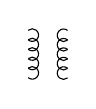
\begin{tikzpicture}
			\draw[black] (0,0) arc(-130:130:0.08);
			\draw[black] (0,0.12) arc(-130:130:0.08);
			\draw[black] (0,0.24) arc(-130:130:0.08);
			\draw[black] (0,0.36) arc(-130:130:0.08);
			\draw[black] (0,0.48) arc(-130:130:0.08);
			
			\draw[black] (0.5,0.12) arc(50:310:0.08);
			\draw[black] (0.5,0.24) arc(50:310:0.08);
			\draw[black] (0.5,0.36) arc(50:310:0.08);
			\draw[black] (0.5,0.48) arc(50:310:0.08);
			\draw[black] (0.5,0.60) arc(50:310:0.08);
		\end{tikzpicture}
	};
	\node[above= 0.0cm of transf, font=\scriptsize]() {Trafo};
	
	\node[draw, minimum width=2cm, minimum height=0.8cm, align=center, below=of power, font=\scriptsize] (pwm) {PWM\\STEUERUNG};
	\node[draw, minimum width=2cm, minimum height=0.8cm, align=center, right=of transf, font=\scriptsize] (rect2) {GLEICHRICHTER\\\& FILTER};
	
	% secutiry
	\node[draw, right=of pwm] (opto) {
		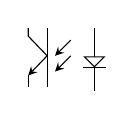
\begin{tikzpicture}
			\draw(0.01,1) -- (0.01,0.9) -- (0.25,0.65);
			\draw[->, >=stealth] (0.25, 0.65) -- (0.01,0.4);
			\draw (0.01,0.4) -- (0.01, 0.25);
			
			\draw(0.25, 1) -- (0.25, 0.25);
			
			\draw[->, >=stealth] (0.55, 0.85) -- ++ (-0.2, -0.2);
			\draw[->, >=stealth] (0.55, 0.65) -- ++ (-0.2, -0.2);
			
			\draw[->, >=open triangle 90] (0.85,1) -- ++ (0, -0.5);
			\draw(0.7, 0.5) -- ++ (0.3, 0);
			\draw (0.85, 0.5) -- (0.85, 0.2);
		\end{tikzpicture}
	};
	
	\node[draw, minimum width=2cm, minimum height=0.8cm, align=center, right=of opto, font=\scriptsize] (detection) {DETEKTIONS-\\SCHALTUNG};
	
	
	% Connections
	\draw (emi.west) ++(-1, 0) -- (emi.west);
	\draw(emi.west) ++(-1.05, 0) circle (2pt) node[above] {I/P};
	\draw (emi) -- (rect1);
	\draw (rect1) -- (power);
	\draw (power) -- (transf);
	\draw (transf) -- (rect2);
	
	
	\begin{scope}[transform canvas={yshift=.6em}]
		\draw[-] (rect2.east) -- ++(1,0) coordinate[pos=0.5] (A);
		\draw (rect2.east) ++(1.05,0) circle (2pt) node[above] {+V};
	\end{scope}
	
	\draw[fill = black] (A) ++(0, .6em) circle (1pt);
	
	\begin{scope}[transform canvas={yshift=-0.6em}]
		\draw[-] (rect2.east) -- ++(1,0);
		\draw(rect2.east) ++(1.05,0) circle (2pt) node[below] {-V};
	\end{scope}
	
	\draw (A) ++ (0,.6em) -- ++ (0, -1) coordinate (B);
	\draw[->] (B) -- ++(-1,0) -- (detection.north);
	\draw [->] (detection) -- (opto);
	\draw [->] (opto) -- (pwm);
	\begin{scope}[transform canvas={xshift=.7em}]
		\draw [->] (pwm)  -- (power);
	\end{scope}
	\begin{scope}[transform canvas={xshift=-0.7em}]
		\draw [->] (power)  -- (pwm);
	\end{scope}
	
}


\newcommand{\batteryConnector} {
	\fill[rounded corners=14pt, ArduinoColor](0,0) rectangle (4,2);
	\fill[ArduinoColor](0,1) rectangle (4,2);
	\fill[ArduinoColor](2,0) rectangle (4,2);
	
	\fill[white] (0.5, 0.5) circle (0.2);
	
	% usb
	\fill[gray!40](0,1.5) rectangle (0.3, 2);
	
	% battery connector
	\fill[brown!40](1.7, 0) rectangle (2.7, 0.8);	
	\fill[brown!20](1.9,0.3) rectangle (2, 0.8);
	\fill[brown!20](2.4,0.3) rectangle (2.5, 0.8);
	\fill[Gold](2,0.8) rectangle ++(0.1, 0.3);
	\fill[Gold](2.3,0.8) rectangle ++(0.1, 0.3);
	
	% other elements
	\fill[black](01, 0.3) rectangle ++(0.5, 0.5);
	\fill[black](1.5, 1) rectangle ++(0.3, 0.3);
	
	% JST Connector
	\fill[brown!40](1.7, -0.2) rectangle ++(1, -0.9);
	\fill[brown!20](1.6, -1.1) rectangle ++(1.2, 0.1);
	\fill[brown!20](2.1, -0.2) rectangle (2.3, -0.8);
	
	% wires
	\draw[red, line width=1.5mm](2.05, -1.1) -- ++(0, -1);
	\draw[black, line width=1.5mm](2.35, -1.1) -- ++(0, -1);
	
	% pins
	\fill[black] (2.9, 0.1) rectangle (4, 0.5);
}

\newcommand{\liIonBattery} { 
	\fill[rounded corners=4pt, gray!40](0,0) rectangle (6,3);
	\fill[ArduinoColor](6,1) rectangle (6.2,2);
	\fill[black](6.05,1.2) rectangle ++(0.1, 0.1);
	\fill[black](6.05,1.8) rectangle ++(0.1, -0.1);
	
	% wires
	\draw[red, line width=1.1mm](6.2, 1.65) -- (8, 1.65);
	\draw[black, line width=1.1mm](6.2, 1.35) -- (8, 1.35);
	
	% JST Connector
	\fill[brown!40](8, 1.2) rectangle (8.8, 1.8);
	\fill[brown!20](8, 1.1) rectangle (8.1, 1.9);
	\fill[brown!20](8.8, 1.4) rectangle ++(-0.4, 0.2);
}



\newcommand{\lorapcbLayout}{
	\node[anchor=south west] (img) at (0,0) {	
\includegraphics[width=11cm]{LoRaPCB/PCBforMKRWAN1310}};
	
	%	\foreach \x in {0,...,11}{
		%		\fill[black] (\x, 0) circle (0.1);
		%		\node at (\x, -0.3) {\x};
		%	}
	%	
	%	\foreach \x in {0,...,11}{
		%		\fill[black] (\x, 8.7) circle (0.1);
		%		\node at (\x, 9) {\x};
		%	}
	%	
	%	\foreach \y in {0,...,9}{
		%		\fill[black] (0, \y) circle (0.1);
		%		\node at (-0.3, \y) {\y};
		%	}
	
	%	
	%	% Battery Section
	%	\draw[red, ultra thick] (5, 7.25) rectangle (8.1, 8.2);
	%	\draw[red, ->, thick, >=angle 60] (5.3, 9) node[above] {\small\shortstack{Akkuanschlüsse und \\ Spannungsteiler}} -- (5.5, 8.3);
	%	
	%	% 230V Input
	%	\draw[red, ultra thick](7.8,2.0) rectangle ++(2,1.3);
	%	\draw[red, ->, thick, >=angle 60] (7.5, -0.5) node[below] {\small Eingang für Netzstrom} -- (7.8, 1.9);
	%
	%	% LED
	%	\draw[red, ultra thick](3.2, 7.15) rectangle (4.8, 8.2);	
	%	\draw[red, ->, thick,  >=angle 60] (2.7, 9) node[above] {\small LED Anschluss} -- (3.3, 8.3);	
	%	
	%		% Widerstände
	%	\draw[red, ultra thick](1.8, 5) rectangle (2.5, 6.6);	
	%	\draw[red, ->, thick,  >=angle 60] (0.7, 7) node[left] {\small\shortstack{Widerstände \\ für LED}} -- (1.7, 6.5);	
	%	
	%	% Analog Sensor
	%	\draw[red, ultra thick](9.6,4.2) rectangle ++(1.5, 0.9);
	%	\draw[red, ->, thick,  >=angle 60] (12, 0) node[below] {\small\shortstack{Eingang für \\ analogen Sensor}} -- (10.5, 4.1);
	%	
	%	% Resistor R10
	%	\draw[red, ultra thick](6.05, 5.9) rectangle ++(0.7, 0.6);
	%	\draw[red, ->, thick,  >=angle 60] (4.4, -0.5) node[below] {\small\shortstack{Analog Signal \\ pull-down \\ Widerstand}} -- (6.3, 5.8);
	%	
	%	% One Line Sensor
	%	\draw[red, ultra thick](9.6,6.3) rectangle ++(1.5, 0.85);
	%	\draw[red, ->, thick,  >=angle 60] (12, 9) node[above] {\small\shortstack{Eingang für \\ One Line Sensor}} -- (10.5, 7.2);
	%	
	%	% Resistor R11
	%	\draw[red, ultra thick](9.9, 5.75) rectangle ++(0.7, 0.6);
	%	\draw[red, ->, thick,  >=angle 60] (12.2, 5) node[below] {\small\shortstack{One Line Sig.\\ pull-up \\ Widerstand}} -- (10.6, 5.75);
	%	
	%	
	%	%CT Sensor
	%	\draw[red, ultra thick] (8.2, 7.15) -- (7.6, 7.15) -- (7.6, 6.5) -- (8.6, 6.5) -- (8.6, 7.15) --(10.3, 7.15) -- (10.3, 8.2) -- (8.2, 8.2) -- (8.2, 7.15);
	%	\draw[red, ->, thick,  >=angle 60] (8.8, 9) node[above] {\small\shortstack{Schaltung und \\ Eingang für Stromsensor}} -- (9, 8.3);
	%%	
	%	% RTC
	%	\draw[red, ultra thick](1.3, 7.15) rectangle (3, 8.2);	
	%	\draw[red, ->, thick,  >=angle 60] (0.5, 9) node[above, left] {\small RTC} -- (1.2, 8.3);	
	%	
	%	% Power Supply
	%	\draw[red, ->, thick,  >=angle 60] (0.7, 1) node[below, left] {\small AC/DC Wandler} -- (2.5, 2);
	%	
	%	% 5V Voltage Divider
	%	\draw[red, ultra thick](4.5, 5.3) rectangle (5.3, 6.5);	   
	%	\draw[red, ->, thick,  >=angle 60] (1.5,-0.5) node[below] {\small\shortstack{Spannungsteiler\\ zur Erkennung\\5V Eingangsspannung}}  -- (4.8, 5.2);	
	%		
	%	% Fuse
	%	\draw[red, ->, thick,  >=angle 60] (10, -1) node[below] {\small Sicherung} -- (9, 1.2);	
	%	
	%	% Arduino
	%	\draw[red, ->, thick, >=angle 60] (0,5.5) node[above] {\small\shortstack{Arduino MKR\\WAN 1310}} -- (1, 3.5);
	%	
	%	% pull-down resistors
	%	\draw[red, ultra thick](2.77,2.3) rectangle ++(0.55,0.65);	
	%	\draw[red, ->, thick, >=angle 60] (-0.2, 2.6) node[left] {\small\shortstack{Pull-down \\ Widerstände}} -- (2.7,2.6);
}

\newcommand{\batteryToArduinoCable}{
	% wires
	\draw[red, line width=1.1mm](4, 1.35) -- (8, 1.65);
	\draw[black, line width=1.1mm](4, 1.65) -- (8, 1.35);
	
	% JST Connector left
	\fill[brown!40](4, 1.2) rectangle (3.2, 1.8);
	\fill[brown!20](4, 1.1) rectangle (3.9, 1.9);
	\fill[brown!20](3.2, 1.4) rectangle ++(0.4, 0.2);
	
	% JST Connector right
	\fill[brown!40](8, 1.2) rectangle (8.8, 1.8);
	\fill[brown!20](8, 1.1) rectangle (8.1, 1.9);
	\fill[brown!20](8.8, 1.4) rectangle ++(-0.4, 0.2);
}


\newcommand{\LoRaWANinfrastructureLabel}{
	% Styl prostokątów
	\fill[gray!10, rounded corners=5] (0,0) rectangle (22,10);
	
	\foreach \x in {5.5, 11, 16.5}{
		\draw[thick, gray!30] (\x, 0) -- (\x,10);
	}
	
	%Boxes witn names
	\node[draw=black, anchor=center, fill=blue!10, rounded corners=3] (endNodes) at (2.75,9.5) {Endgeräte};
	\node[draw=black, anchor=center, fill=blue!10, rounded corners=3] (gateway) at (8.25,9.5) {Gateway};
	\node[draw=black, anchor=center, fill=blue!10, rounded corners=3] (NetServ) at (13.75,9.5) {Netzwerkserver};
	\node[draw=black, anchor=center, fill=blue!10, rounded corners=3] (AppServ) at (19.25,9.5) {Applikationsserver};
	
	% end nodes
	\node[draw=blue!70!black, circle,fill=blue!10, minimum size=0.6cm] (end1) at (3.8,8) {Sensor 1};
	\node[draw=blue!70!black, circle,fill=blue!10, minimum size=0.6cm] (end2) at (2.0,6.9) {Sensor 2};
	\node[draw=blue!70!black, circle,fill=blue!10, minimum size=0.6cm] (end3) at (1.1,5) {Sensor 3};
	\node[draw=blue!70!black, circle,fill=blue!10, minimum size=0.6cm] (end4) at (2.0,3.1) {Sensor 4};	
	\node[draw=blue!70!black, circle,fill=blue!10, minimum size=0.6cm] (end5) at (3.8,2) {Sensor 5};
	
	%gateways	
	\node[draw=blue!70!black, shape=regular polygon, regular polygon sides=6, shape border uses incircle, minimum size=2cm, fill=blue!10] (gat1) at (7.1,7) {Gat 1};
	\node[draw=blue!70!black, shape=regular polygon, regular polygon sides=6, shape border uses incircle, minimum size=2cm, fill=blue!10] (gat2) at (8.5,5) {Gat 2};
	\node[draw=blue!70!black, shape=regular polygon, regular polygon sides=6, shape border uses incircle, minimum size=2cm, fill=blue!10] (gat3) at (7.1,3) {Gat 3};
	
	%Network server
	\node[draw=blue!70!black, cloud, fill=blue!10, minimum width=5cm, minimum height=2cm] (NS) at (13.75,5) {Netzwekserver};
	
	% applications
	\node[draw=blue!70!black, rectangle,fill=blue!10, minimum size=1cm] (app1) at (19.25,7) {Anwendung 1};
	\node[draw=blue!70!black, rectangle,fill=blue!10, minimum size=1cm] (app2) at (19.25,3) {Anwendung 2};	
	
	%====== connections ========
	% end punkt -- gateway
	\foreach \s in {end1, end2, end3, end4, end5}{
		\draw[dashed, orange, thick] (\s.east) -- (gat1.west);
		\draw[dashed, orange, thick] (\s.east) -- (gat2.west);
		\draw[dashed, orange, thick] (\s.east) -- (gat3.west);
	}
	
	
	% gateway -- server
	\draw[thick] ($(gat1.east)+(0.2,0)$) -- ++(0.5,0) -- (10.25,7);
	\draw[thick] ($(gat3.east)+(0.2,0)$) -- ++(1.9,0) -- (10.25,7);
	\draw[thick] ($(gat2.east)+(0.2,0)$) -- ($(NS.west)-(0.2,0)$);
	
	% server -- apps
	\draw[thick] ($(NS.east)+(0.2,0)$) -- (17.4,5);
	\draw[thick] ($(app1.west) - (0.2,0)$) -- ++(-0.5,0) -- (17.4,5);
	\draw[thick] ($(app2.west) - (0.2,0)$) -- ++(-0.5,0) -- (17.4,5);	
	
	
	% Connunication types
	\draw[fill=white!30, rounded corners=3] (1,0.2) rectangle (8,1) node[pos=.5]{LoRa};
	\draw[fill=white!30, rounded corners=3] (8.5,0.2) rectangle (20,1) node[pos=.5]{TCP/IP};
	
}

\newcommand{\LoRaWANinfrastructure}{
	% Styl prostokątów
	\fill[gray!10, rounded corners=5] (0,1) rectangle (22,10);
	
	\foreach \x in {5.5, 11, 16.5}{
		\draw[thick, gray!30] (\x, 1) -- (\x,10);
	}
	
	%Boxes witn names
	\node[draw=black, anchor=center, fill=blue!10, rounded corners=3] (endNodes) at (2.75,9.5) {Endgeräte};
	\node[draw=black, anchor=center, fill=blue!10, rounded corners=3] (gateway) at (8.25,9.5) {Gateway};
	\node[draw=black, anchor=center, fill=blue!10, rounded corners=3] (NetServ) at (13.75,9.5) {Netzwerkserver};
	\node[draw=black, anchor=center, fill=blue!10, rounded corners=3] (AppServ) at (19.25,9.5) {Applikationsserver};
	
	% end nodes
	\node[draw=blue!70!black, circle,fill=blue!10, minimum size=0.6cm] (end1) at (3.8,8) {Sensor 1};
	\node[draw=blue!70!black, circle,fill=blue!10, minimum size=0.6cm] (end2) at (2.0,6.9) {Sensor 2};
	\node[draw=blue!70!black, circle,fill=blue!10, minimum size=0.6cm] (end3) at (1.1,5) {Sensor 3};
	\node[draw=blue!70!black, circle,fill=blue!10, minimum size=0.6cm] (end4) at (2.0,3.1) {Sensor 4};	
	\node[draw=blue!70!black, circle,fill=blue!10, minimum size=0.6cm] (end5) at (3.8,2) {Sensor 5};
	
	%gateways	
	\node[draw=blue!70!black, shape=regular polygon, regular polygon sides=6, shape border uses incircle, minimum size=2cm, fill=blue!10] (gat1) at (7.1,7) {Gat 1};
	\node[draw=blue!70!black, shape=regular polygon, regular polygon sides=6, shape border uses incircle, minimum size=2cm, fill=blue!10] (gat2) at (8.5,5) {Gat 2};
	\node[draw=blue!70!black, shape=regular polygon, regular polygon sides=6, shape border uses incircle, minimum size=2cm, fill=blue!10] (gat3) at (7.1,3) {Gat 3};
	
	%Network server
	\node[draw=blue!70!black, cloud, fill=blue!10, minimum width=5cm, minimum height=2cm] (NS) at (13.75,5) {Netzwekserver};
	
	% applications
	\node[draw=blue!70!black, rectangle,fill=blue!10, minimum size=1cm] (app1) at (19.25,7) {Anwendung 1};
	\node[draw=blue!70!black, rectangle,fill=blue!10, minimum size=1cm] (app2) at (19.25,3) {Anwendung 2};	
	
	%====== connections ========
	% end punkt -- gateway
	\foreach \s in {end1, end2, end3, end4, end5}{
		\draw[dashed, orange, thick] (\s.east) -- (gat1.west);
		\draw[dashed, orange, thick] (\s.east) -- (gat2.west);
		\draw[dashed, orange, thick] (\s.east) -- (gat3.west);
	}
	
	
	% gateway -- server
	\draw[thick] ($(gat1.east)+(0.2,0)$) -- ++(0.5,0) -- (10.25,7);
	\draw[thick] ($(gat3.east)+(0.2,0)$) -- ++(1.9,0) -- (10.25,7);
	\draw[thick] ($(gat2.east)+(0.2,0)$) -- ($(NS.west)-(0.2,0)$);
	
	% server -- apps
	\draw[thick] ($(NS.east)+(0.2,0)$) -- (17.4,5);
	\draw[thick] ($(app1.west) - (0.2,0)$) -- ++(-0.5,0) -- (17.4,5);
	\draw[thick] ($(app2.west) - (0.2,0)$) -- ++(-0.5,0) -- (17.4,5);	
	
}

\newcommand{\LoRaWANBAckendinfrastructure}{
	% Styl prostokątów
	\fill[gray!10, rounded corners=5] (0,0) rectangle (17,9);
	
	
	%gateways	
	\node[draw=blue!70!black, shape=regular polygon, regular polygon sides=6, shape border uses incircle, minimum size=2cm, fill=blue!10] (gat1) at (2,7) {Gateway};
	
	%Network server
	\node[draw=blue!70!black, cloud, fill=blue!10, minimum width=4cm, minimum height=3cm, inner sep=0pt] (NS) at (8,7) {\shortstack{Netzwek-\\server}};
	
	\node[draw=blue!70!black, cloud, fill=blue!10, minimum width=4cm, minimum height=3cm, inner sep=0pt, right = 2.5cm of NS] (AS) {\shortstack{Anwendungs-\\server}};
	\node[draw=blue!70!black, cloud, fill=blue!10, minimum width=4cm, minimum height=3cm, inner sep=0pt, below = 2cm of NS] (JS) {\shortstack{Join\\server}};
	
	\draw[thick] ($(gat1.east)+(0.2,0)$) -- ($(NS.west)-(0.2,0)$);
	\draw[thick] ($(NS.east)+(0.2,0)$) -- ($(AS.west)-(0.2,0)$);
	\draw[thick] ($(NS.south)+(0,-0.2)$) -- ($(JS.north)+(0,0.2)$);
	\draw[thick] ($(AS.south west)+(0,-0.2)$) -- ($(JS.north east)+(0,0.2)$);
	
}

% #1 = scale
% #2 = angle
% #3 = x coordinate
% #4 = y coordinate
% #5 = name
\newcommand{\server}[5]{
	\begin{scope}[shift={(#3, #4)}]
		\begin{scope}[scale=#1, rotate=#2]
			
			
			
			\fill[gray] (-0.7, -0.7) rectangle (0.7, -1.2);
			\fill[gray] (-0.7, 0.7) rectangle (0.7, 1.2);
			
		\end{scope}
	\end{scope}
}


% #1 = scale
% #2 = angle
% #3 = x coordinate
% #4 = y coordinate
% #5 = colour
\newcommand{\smallSMDResistor}[5]{
	\begin{scope}[shift={(#3, #4)}]
		\begin{scope}[scale=#1, rotate=#2]
			
			\fill[gray!30] (-1, -1.8) rectangle (1, 1.8);
			\fill[#5] (-1, -0.1) rectangle (1, 0.1);
			
			\fill[black] (-0.7, -0.7) rectangle (0.7, 0.7);
			
			\fill[gray] (-0.7, -0.7) rectangle (0.7, -1.2);
			\fill[gray] (-0.7, 0.7) rectangle (0.7, 1.2);
			
		\end{scope}
	\end{scope}
}

% #1 = scale
% #2 = angle
% #3 = x coordinate
% #4 = y coordinate
% #5 = colour
\newcommand{\smallSMDCapacitor}[5]{
	\begin{scope}[shift={(#3, #4)}]
		\begin{scope}[scale=#1, rotate=#2]
			
			\fill[gray!30] (-1, -1.8) rectangle (1, 1.8);
			\fill[#5] (-1, -0.1) rectangle (1, 0.1);
			
			\fill[brown!30] (-0.7, -0.7) rectangle (0.7, 0.7);
			
			\fill[gray] (-0.7, -0.7) rectangle (0.7, -1.2);
			\fill[gray] (-0.7, 0.7) rectangle (0.7, 1.2);
			
		\end{scope}
	\end{scope}
}

% #1 = scale
% #2 = angle
% #3 = x coordinate
% #4 = y coordinate
\newcommand{\SMDtransistor}[4]{
	\begin{scope}[shift={(#3, #4)}]
		\begin{scope}[scale=#1, rotate=#2]
			
			\fill[black] (-1, -1.8) rectangle (1, 1.8);
			
			\fill[gray!30] (-1, -1.8) rectangle ++(-1.2, 1.2);
			\fill[gray!30] (-1, 1.8) rectangle ++(-1.2, -1.2);
			\fill[gray!30] (1, -0.6) rectangle ++(1.2, 1.2);
			
			\fill[gray] (-0.8, -1.5) rectangle ++(-0.6, 0.6);
			\fill[gray] (-0.8, 1.5) rectangle ++(-0.6, -0.6);
			\fill[gray] (0.8, -0.3) rectangle ++(0.6, 0.6);
		\end{scope}
	\end{scope}
}

% #1 = scale
% #2 = angle
% #3 = x coordinate
% #4 = y coordinate
% #5 = colour
\newcommand{\SMDLed}[5]{
	\begin{scope}[shift={(#3, #4)}]
		\begin{scope}[scale=#1, rotate=#2]
			
			\fill[gray!30] (-0.7, -1.8) rectangle (0.7, 1.8);
			\fill[#5] (0,0) circle (1cm);
		\end{scope}
	\end{scope}
}

% #1 = scale
% #2 = angle
% #3 = x coordinate
% #4 = y coordinate
% #5 = enable pin labels (1 - on / 0 - off)
% Every pin has a node in center -> mkrPin-XX (XX -> pin number/name)
\newcommand{\ArduinoMkrWan}[5]{
	\begin{scope}[shift={(#3, #4)}]	
		\tikzset{
			lineScaled/.style n args={1}			{line width={#1*3pt}},
			thinLineScaled/.style n args={1}		{line width={#1*0.8pt}},
			cornersBigScaled/.style n args = {1} 	{rounded corners={#1*10pt}},
			cornersSmallScales/.style n args = {1}	{rounded corners={#1*5pt}},
		}
		\begin{scope}[scale=#1, rotate=#2, transform shape]			
			% Grid for the picture
			
			%\foreach \x in {-5,...,5} {
				%	\fill[red] (\x, -11) circle (0.2);
				%	\node[red] at (\x, -11.8) {\Large \x};
				
				%	\fill[red] (\x, 11) circle (0.2);
				%	\node[above, red] at (\x, 11.8) {\Large \x};
				%}
			
			%\foreach \y in {-10,...,10} {
				%	\fill[red] (-4.5, \y) circle (0.2);
				%	\node[left, red] at (-5.2, \y) {\Large \y};
				%}
			
			%==========  TIKZ  ==================
			\fill[ArduinoColor, cornersBigScaled=#1] (-3.6, -9.6) rectangle (3.6, 10);
			% Drills
			\foreach \x in {-3, 3} {
				\foreach \y in {-8.9, 7.6} {
					\fill[white] (\x, \y) circle (0.35);
				}
			}
			
			% Pin Headers
			\foreach \x in {-3.3, 2.6} {
				\fill[black] (\x, -3.5) rectangle ({\x+0.7}, 6.8);
				
				% 14 gray pins
				\foreach \i in {0,...,13} {
					\pgfmathsetmacro{\y}{-3.45 + \i*0.735}
					\fill[gray] ({\x+0.2}, {\y+0.2}) rectangle ({\x+0.5}, {\y+0.5});
				}
			}
			
			%%%%%%%%%%%%%%%%%%%%%%
			% LABELS
			%%%%%%%%%%%%%%%%%%%%%%
			\foreach \i/\label in {
				0/5V, 1/VIN, 2/VCC, 3/GND, 4/RESET, 5/14, 6/13, 
				7/12, 8/11, 9/10, 10/9, 11/8, 12/7, 13/6
			} {
				\pgfmathsetmacro{\x}{-3.3+0.35}
				\pgfmathsetmacro{\y}{-3.45 + \i*0.735 + 0.35}
				
				% not visible point in the middle of grey square
				\node[inner sep=0pt, outer sep=0pt, minimum size=0pt, draw=none] (mkrPin-\label) at (\x,\y) {};
				
				% text description
				\ifnum#5=1
				\node[font=\sffamily\large, anchor=east, xshift=-0.7cm]
				at (mkrPin-\label) {\label};
				\fi
			}
			
			\foreach \i/\label in {
				0/AREF, 1/A0, 2/A1, 3/A2, 4/A3, 5/A4, 6/A5, 
				7/A6, 8/0, 9/1, 10/2, 11/3, 12/4, 13/5
			} {
				% środek kwadracika
				\pgfmathsetmacro{\x}{2.6+0.35}
				\pgfmathsetmacro{\y}{-3.45 + \i*0.735 + 0.35}
				
				% niewidoczny punkt w środku, nazwany wg etykiety
				\node[inner sep=0pt, outer sep=0pt, minimum size=0pt, draw=none] (mkrPin-\label) at (\x,\y) {};
				
				
				% etykieta tekstowa obok
				\ifnum#5=1
				\node[font=\sffamily\large, anchor=west, xshift=0.7cm]
				at (mkrPin-\label) {\label};
				\fi
			}
			
			
			
			% USB Port
			\fill[gray!30] (-1.1, -10) rectangle (1.1, -8.3);
			
			\foreach \i in {0,...,4} {
				\pgfmathsetmacro{\x}{-0.38 + \i*0.2}
				\fill[gray] ({\x-0.08}, -8.3) rectangle ({\x+0.08}, -8.1);
			}
			
			
			%I2C Connector
			\fill[brown!40] (-3.7, -8.4) rectangle (-2.4, -6.1);
			
			\foreach \i in {0,...,4} {
				\pgfmathsetmacro{\y}{-7.87 + \i*0.34}
				\fill[gray] (-2.4, {\y-0.04}) rectangle (-2.2, {\y+0.04});
			}
			
			% Battery Connector
			\fill[brown!40] (2, -6.8) rectangle (3.7, -4.3);
			
			\foreach \i in {0,...,1} {
				\pgfmathsetmacro{\y}{-5.82 + \i*0.6}
				\fill[gray] (1.2, {\y-0.07}) rectangle (2, {\y+0.07});
			}
			
			% CPU
			\fill[black] (-1.1, -3.2) rectangle (0.95, -1.2);
			
			\foreach \x in {-1.1, 0.95} {
				\foreach \i in {0,...,10} {
					\pgfmathsetmacro{\y}{-3.05 + \i*0.17}
					\fill[gray] ({\x-0.08}, {\y-0.05}) rectangle ({\x+0.08}, {\y+0.05});
				}
			}
			
			\foreach \y in {-3.2, -1.2} {
				\foreach \i in {0,...,10} {
					\pgfmathsetmacro{\x}{-0.94 + \i*0.17}
					\fill[gray] ({\x-0.05}, {\y-0.08}) rectangle ({\x+0.05}, {\y+0.08});
				}
			}
			
			% Smaller chip
			\fill[black] (1.65, -8.2) rectangle (2.85, -7.05);
			
			\foreach \x in {1.65, 2.85} {
				\foreach \i in {0,...,7} {
					\pgfmathsetmacro{\y}{-8.1 + \i*0.135}
					\fill[gray] ({\x-0.07}, {\y-0.035}) rectangle ({\x+0.07}, {\y+0.035});
				}
			}
			
			\foreach \y in {-8.2, -7.05} {
				\foreach \i in {0,...,7} {
					\pgfmathsetmacro{\x}{1.775 + \i*0.135}
					\fill[gray] ({\x-0.035}, {\y-0.07}) rectangle ({\x+0.035}, {\y+0.07});
				}
			}
			
			% LoRa Module
			\fill[black] (-1.7, 3.15) rectangle (1.7, 6.75);
			\fill[gray] (-1.6, 3.45) -- (-1.6, 6.45) -- (-1.4, 6.65) -- (1.4, 6.65) -- (1.6, 6.45) -- (1.6, 3.45) -- (1.4, 3.25) -- (-1.4, 3.25) -- (-1.6, 3.45);
			
			% LoRa Antenna
			\fill[gray] (-1.6, 8.3) rectangle ++(1.2, 1.2);
			\fill[Gold] (-1.0, 8.9) circle (0.12cm);
			\draw[lineScaled=#1, Gold] (-1.0, 8.9) circle (0.45cm);
			
			% Small elements on the board going from the top
			\foreach \x in {-1.55, -1.25} {
				\foreach \y in {7.68, 8.08} {
					\pgfmathsetmacro{\i}{0.10}
					\fill[gray] ({\x-\i}, {\y-\i}) rectangle ({\x+\i}, {\y+\i});
				}
			}
			
			% Chip 1
			\fill[black] (0.9, 0.6) rectangle (2.2, 2.2);
			
			\foreach \y in {0.5, 2.3} {
				\foreach \i in {0,...,3} {
					\pgfmathsetmacro{\x}{1 + \i*0.35}
					\fill[gray] ({\x-0.07}, {\y-0.15}) rectangle ({\x+0.07}, {\y+0.15});
				}
			}
			
			% Chip 2
			\fill[black] (-1.05, -0.7) rectangle (-0.2, -0.05);
			
			\foreach \x in {-1.08, -0.17} {
				\foreach \i in {0,...,3} {
					\pgfmathsetmacro{\y}{-0.6 + \i*0.15}
					\fill[gray] ({\x-0.04}, {\y-0.06}) rectangle ({\x+0.04}, {\y+0.06});
				}
			}
			
			
			% Chip 3
			\fill[gray] (1.25, -0.87) rectangle (2.1, -0.48);
			\draw[gray!30, lineScaled=#1] (1.5, -0.4) -- ++(-0.32, 0) -- ++(0, -0.55) -- ++(0.32, 0);
			\draw[gray!30, lineScaled=#1] (1.85, -0.4) -- ++(0.32, 0) -- ++(0, -0.55) -- ++(-0.32, 0);
			
			%Chip 4
			\fill[black] (1.42, -4.05) rectangle (1.84, -3.2);
			
			\foreach \i in {0, 1, 2} {
				\pgfmathsetmacro{\x}{1.39}
				\pgfmathsetmacro{\y}{-3.855 + \i*0.24}
				\fill[gray] ({\x-0.1}, {\y-0.04}) rectangle ({\x+0.1}, {\y+0.04});
			}
			
			\foreach \i in {0,1} {
				\pgfmathsetmacro{\x}{1.87}
				\pgfmathsetmacro{\y}{-3.855 + \i*0.48}
				\fill[gray] ({\x-0.1}, {\y-0.04}) rectangle ({\x+0.1}, {\y+0.04});
			}
			
			
			% Button
			\fill[gray!30] (-0.7, -4.95) rectangle (0.6, -4.12);
			\fill[white] (-0.05, -4.5) circle (0.25cm);
			
			\foreach \x in {-0.5, 0.4}{
				\foreach \y in {-5, -4.08} {
					\fill[gray] ({\x-0.1}, {\y-0.05}) rectangle ({\x+0.1}, {\y+0.05});
				}	
			}
			
			% Chip 5
			\fill[black, cornersSmallScales] (-2.05, -5.9) rectangle (-0.9, -4.85);
			
			\foreach \y in {-6.0, -4.75} {
				\pgfmathsetmacro{\x}{-1.475}
				\fill[gray] ({\x-0.2}, {\y-0.1}) rectangle ({\x+0.2}, {\y+0.1});
			}
			
			
			% Chip 6
			\fill[black] (-0.3, -8.0) rectangle (0.22, -7.22);
			\foreach \x in {-0.35, 0.27}{
				\foreach \y in {-7.85, -7.37} {
					\fill[gray] ({\x-0.15}, {\y-0.06}) rectangle ({\x+0.15}, {\y+0.06});
				}	
			}
			% Chip 7
			\fill[green!30!black] (0.4, -7.2) rectangle (1, -6.55);   
			
			\foreach \x in {0.36, 1.04} {
				\foreach \i in {0,...,2} {
					\pgfmathsetmacro{\y}{-7.06 + \i*0.20}
					\fill[gray] ({\x-0.04}, {\y-0.06}) rectangle ({\x+0.04}, {\y+0.06});
				}
			}
			
			% Resistors
			\smallSMDResistor{0.12}{0}{-0.96}{7.86}{ArduinoColor}
			\smallSMDResistor{0.12}{90}{-0.81}{7.18}{ArduinoColor}
			\smallSMDResistor{0.12}{0}{2.1}{5.3}{ArduinoColor}
			\smallSMDResistor{0.12}{0}{2.1}{4.6}{ArduinoColor}
			\smallSMDResistor{0.12}{0}{-2.1}{3.8}{ArduinoColor}
			\smallSMDResistor{0.12}{0}{-2.1}{4.5}{ArduinoColor}
			
			\foreach \x in {-1.16, -0.57, 0.02, 1.18} {
				\smallSMDResistor{0.12}{90}{\x}{2.65}{ArduinoColor}
			}
			\smallSMDResistor{0.12}{90}{-1.16}{2.25}{ArduinoColor}
			\smallSMDResistor{0.12}{0}{-0.40}{2.0}{ArduinoColor}
			
			\smallSMDResistor{0.2}{90}{-1}{1.8}{ArduinoColor}
			\smallSMDResistor{0.2}{0}{0.0}{1.8}{ArduinoColor}
			
			\foreach \y in {1.05, 0.7} {
				\smallSMDResistor{0.12}{90}{0.4}{\y}{ArduinoColor}
			}
			
			\smallSMDResistor{0.2}{90}{0}{0.25}{ArduinoColor}
			\smallSMDResistor{0.2}{90}{0.6}{-0.24}{ArduinoColor}
			
			\foreach \x in {1.36, 1.97} {
				\smallSMDResistor{0.12}{90}{\x}{-0.16}{ArduinoColor}
			}
			
			\foreach \y in {0.1, -0.2} {
				\smallSMDResistor{0.12}{90}{-1.75}{\y}{ArduinoColor}
			}
			
			\foreach \x in {-2.4, -2.08} {
				\foreach \y in {-0.71, -1.27 } {
					\smallSMDResistor{0.12}{0}{\x}{\y}{ArduinoColor}
				}
			}
			\smallSMDResistor{0.12}{0}{-1.3}{-0.71}{ArduinoColor}
			
			\smallSMDResistor{0.12}{90}{-1.75}{-2.08}{ArduinoColor}
			\smallSMDResistor{0.12}{90}{-2.24}{-2.43}{ArduinoColor}
			
			\foreach \y in {-1.72, -2.05, -2.38} {
				\smallSMDResistor{0.12}{90}{1.98}{\y}{ArduinoColor}
			}
			
			\smallSMDResistor{0.12}{90}{1.38}{-2.05}{ArduinoColor}
			
			\foreach \y in {-2.97, -3.62} {
				\smallSMDResistor{0.12}{0}{2.31}{\y}{ArduinoColor}
			}
			
			\foreach \y in {-3.61, -4.23} {
				\smallSMDResistor{0.12}{0}{1.02}{\y}{ArduinoColor}
			}
			
			\foreach \y in {-3.75, -4.26} {
				\smallSMDResistor{0.2}{90}{-1.47}{\y}{ArduinoColor}
			}
			
			
			\foreach \x in {-2.3} {
				\foreach \y in {-3.6} {
					\smallSMDResistor{0.2}{0}{\x}{\y}{ArduinoColor}
					\draw[white, thinLineScaled=#1] ({\x-0.06}, {\y-0.09}) rectangle ({\x+0.06}, {\y+0.09});
				}
			}
			
			\smallSMDResistor{0.12}{90}{-3.15}{-5.35}{ArduinoColor}
			\smallSMDResistor{0.12}{90}{-1.48}{-6.3}{ArduinoColor}
			
			\foreach \y in {-6.8, -7.3, -8.25} {
				\smallSMDResistor{0.12}{0}{-1.49}{\y}{ArduinoColor}
			}
			
			\smallSMDResistor{0.2}{0}{-1.95}{-8.1}{ArduinoColor}
			\smallSMDResistor{0.2}{0}{-1.05}{-6.9}{ArduinoColor}
			\smallSMDResistor{0.2}{0}{-0.55}{-6.75}{ArduinoColor}
			\smallSMDResistor{0.12}{0}{0.13}{-6.75}{ArduinoColor}
			
			\foreach \x in {0.55} {
				\foreach \y in {-6.23} {
					\smallSMDResistor{0.2}{90}{\x}{\y}{ArduinoColor}
					\draw[white, thinLineScaled=#1] (\x,\y) ellipse [x radius=1mm, y radius=0.5mm];
				}
			}
			
			\smallSMDResistor{0.12}{90}{1.36}{-6.2}{ArduinoColor}
			\smallSMDResistor{0.12}{0}{1.35}{-6.7}{ArduinoColor}
			\smallSMDResistor{0.12}{90}{0.7}{-7.62}{ArduinoColor}
			\smallSMDResistor{0.12}{90}{1.23}{-8.15}{ArduinoColor}
			\smallSMDResistor{0.12}{90}{3.23}{-8.15}{ArduinoColor}
			\smallSMDResistor{0.12}{0}{1.35}{-8.6}{ArduinoColor}
			
			\foreach \y in {-7.05, -7.6} {
				\smallSMDResistor{0.12}{0}{3.37}{\y}{ArduinoColor}
			}
			
			% Transistors
			\SMDtransistor{0.12}{180}{-3.15}{-4.85}
			\SMDtransistor{0.12}{0}{-1}{-7.75}
			
			% LEDs
			\SMDLed{0.22}{0}{1.8}{-9.07}{orange}
			\SMDLed{0.22}{0}{-1.9}{-9.07}{green}
			\SMDLed{0.22}{90}{-2.95}{-4.1}{orange}
			
			%Image of MKR WAN 1310
			%\node[anchor=center, inner sep=0pt, opacity=0.3] at (0,0) {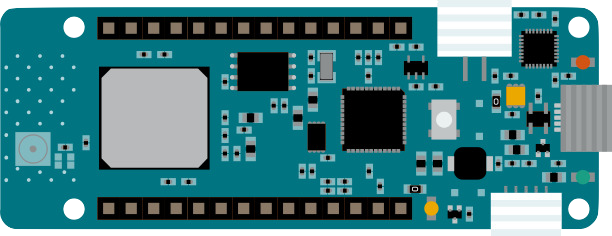
\includegraphics[width=20cm, angle=270]{../Images/MKRWAN1310/mkrwan1310}};
		\end{scope}
	\end{scope}
}


% #1 = 1. strip
% #2 = 2. strip
% #3 = 3. strip
% #4 = 4. strip
\newcommand{\coloursOnResistor}[5]{%
	\tikzset{
		scaledCorners/.style n args={1}{rounded corners={#1*3pt}}
		%scaledCorners/.style n args={1}{rounded corners={7pt}}
	}
	
	\def\noval{none}
	
	% first strip
	\def\cA{#2}%
	\ifx\cA\noval\else
	\fill[\cA, scaledCorners] (-2.0,-1.2) rectangle (-1.6,1.2);
	\fi
	
	% second strip
	\def\cB{#3}%
	\ifx\cB\noval\else
	\fill[\cB] (-1,-1) rectangle (-0.6,1);
	\fi
	
	% third strip
	\def\cC{#4}%
	\ifx\cC\noval\else
	\fill[\cC] (0,-1) rectangle (0.4,1);
	\fi
	
	% fourth strip
	\def\cD{#5}%
	\ifx\cD\noval\else
	\fill[\cD, scaledCorners] (2.0,-1.2) rectangle (1.6,1.2);
	\fi
}

%%%%%%%%%%%%%%%%%%%%%%%%%%%%%%%%%%%%%%%%%%%%%%%%%%%%%%%%%%%%%%%%%%%%%%
% #1 = scale
% #2 = angle
% #3 = x coordinate
% #4 = y coordinate
% #5 = Resistor Value
% #6 = Resistor Identificator

% Nodes:
%(RES-LEFT-#6)
%(RES-RIGHT-#6)
\newcommand{\resistorTHT}[6]{
	\begin{scope}[shift={(#3, #4)}]
		\tikzset{
			lineScaled/.style n args={1}{line width={#1*7pt}}
		}
		
		\begin{scope}[scale=#1, rotate=#2]
			
			\fill[brown!40](-2,-1) rectangle (2, 1);
			\fill[brown!40] (-1.8, 0) circle (1.2);
			\fill[brown!40] (1.8, 0) circle (1.2);
			
			\node[inner sep=0pt, outer sep=0pt, minimum size=0pt, draw=none] (RES-LEFT-#6) at (-3,0) {};
			\node[inner sep=0pt, outer sep=0pt, minimum size=0pt, draw=none] (RES-RIGHT-#6) at (3,0) {};
			
			
			% Strips for resistor
			%%%%%%%%%%%%%%%%%%%%%%%%%%%%%%
			%	0 - no strips
			%	1 - 4.7kOhm
			%	2 - 10 kOhm
			%
			%
			%
			
			
			\def\resval{#5}
			
			\ifcase\resval
			% 0: no strips
			\coloursOnResistor{#1}{none}{none}{none}{none}
			\or
			% 1: strips for 4.7k
			\coloursOnResistor{#1}{yellow}{Purple}{red}{brown}
			\or
			% 2: paski dla 10k
			\coloursOnResistor{#1}{brown}{black}{Orange}{Gold}
			\else
			% default
			\coloursOnResistor{#1}{none}{none}{none}{none}
			\fi
			
		\end{scope}
	\end{scope}
}

\newcommand{\protocolsiot}{
	\tikzset{
		lineScaled/.style n args={1}{line width=1pt},
		lineScaledWire/.style n args={1}{line width=9pt},
		arrowStyle/.style={lineScaled=1, >=stealth},
		labelnode/.style n args={1}{scale=1.0},
		nodeStyle/.style ={rounded corners=6pt, thick, blue!60, draw, text=black}
	}
	
	\draw[arrowStyle, <->] (0,6) coordinate(A) -- (0,0) -- (10,0) coordinate(B);
	\node[anchor=south] at (A) {Bandbreite};
	\node[anchor=west, labelnode]  at (B) {Reichweite};
	
	
	\node[nodeStyle, minimum width=2cm, minimum height=1cm, anchor=south west] at (0.2, 0.2) {NFC};
	\node[nodeStyle, minimum width=3cm, minimum height=1cm] at (2.5, 3) {Bluetooth};
	\node[nodeStyle, minimum width=3cm, minimum height=1cm] at (4.5, 1.6) {Zigbee};
	\node[nodeStyle, minimum width=2cm, minimum height=3cm] at (5.5, 4) {WiFi};
	\node[nodeStyle, minimum width=1cm, minimum height=0.8cm] at (7.5, 2) {2G};
	\node[nodeStyle, minimum width=1cm, minimum height=0.8cm] at (7.5, 3) {3G};
	\node[nodeStyle, minimum width=1cm, minimum height=0.8cm] at (7.5, 4) {4G};
	\node[nodeStyle, minimum width=1cm, minimum height=0.8cm] at (7.5, 5) {5G};
	\node[nodeStyle, minimum width=3cm, minimum height=0.8cm, anchor=south] at (8.5, 0.2) {\shortstack{LoRa/ Sigfox \\ NB-IoT / LTE}};
}

\newcommand{\transmittertx}{
	\tikzset{
		lineScaled/.style n args={1}{line width=1pt},
		labelnode/.style n args={1}{scale=1.0},
		nodeStyle/.style ={rounded corners=4pt, thick, draw, text=black}
	}
	
	\node[nodeStyle, fill=green, minimum width=2.5cm, minimum height=1.3cm] (tx) {Sender};
	\node[nodeStyle, fill=red, minimum width=1.5cm, minimum height=0.8cm, right=1cm of tx] (cb) {Leitung};
	
	\node[
	draw,
	thick,
	fill=green,
	isosceles triangle,            
	isosceles triangle apex angle=30,
	shape border rotate=270,       
	minimum height=2.2cm,          
	minimum width=0.1cm,             
	align=center,
	inner sep=0pt
	] (ant) at ($(cb.east) + (1.5cm,1.9cm)$) {\rotatebox{90}{Antenne}};
	
	\draw[lineScaled] (tx) -- (cb);
	\draw[lineScaled] (cb.east) -| (ant.south);
	
	\node[below=0mm of tx] {Gain (dBm)};
	\node[below=0mm of cb] {Loss (dB)};
	\node[left=0mm of ant] {Gain (dBi)};
}

\newcommand{\loraframe}{
	\tikzset{
		defaulttext/.style={
			font=\sffamily\small,
		}
	}
	
	\filldraw[fill=orange!20, draw=black, thick] (0,1) rectangle (3,2);
	\filldraw[fill=orange!20, draw=black, thick] (3,1) rectangle (6,2);
	\filldraw[fill=blue!20, draw=black, thick] (6,1) rectangle (10,2);
	\filldraw[fill=orange!20, draw=black, thick] (10,1) rectangle (11.5,2);
	\draw[black] (3, 1.45) -- (6, 1.45);
	\draw[black ] (5, 1.45) -- (5, 2);
	
	\node[defaulttext] at (1.5,1.5) {\textbf{Preamble}};
	\node[defaulttext] at (4,1.7) {\textbf{Header}};
	\node[defaulttext] at (5.5,1.7) {\textbf{CRC}};
	\node[defaulttext] at (4.5,1.2) {\footnotesize{(explicit mode only)}};
	\node[defaulttext] at (8,1.5) {\textbf{PHY Payload}};
	\node[defaulttext] at (8,1.2) {\small \(p\) bytes};
	\node[defaulttext] at (10.75,1.5) {\shortstack{\textbf{Payload}\\\textbf{CRC}}};
	
	\draw[<->, thick] (0,2.4) -- (11.5,2.4) node[midway, above]{\textbf{Time on Air}};
	
	
}

\newcommand{\lorawanframes}{
	\tikzset{
		defaulttext/.style={
			font=\sffamily\small,
		},
		smallText/.style={
			font=\sffamily\footnotesize,
		},
		defaultDashed/.style={dashed,line width=0.06cm}
	}
	
	% PHY Layer
	\filldraw[fill=orange!20, draw=black, thick] (0, 1) rectangle (13,2);
	\filldraw[fill=blue!20, draw=black, thick] (5,1) rectangle (11,2);
	\foreach \x in {2, 3.5, 5, 11} {
		\draw[thick] (\x, 1) -- (\x, 2);
	}
	\node[defaulttext] at (1,1.5) {\textbf{Preamble}};
	\node[defaulttext] at (2.75,1.5) {\textbf{Header}};
	\node[defaulttext] at (4.25,1.5) {\textbf{CRC}};
	\node[defaulttext] at (8,1.5) {\textbf{PHY Payload}};
	\node[defaulttext] at (12,1.5) {\shortstack{\textbf{Payload}\\\textbf{CRC}}};
	
	% PHY Payload
	\phyPayload
	
	% MACPayload		
	\macPayload
	
	% FHDR
	\fhdrHeader
	
	% Names
	%\node[defaulttext] at (0.5,-6) {\textbf{FHDR}};
	%\node[defaulttext] at (1,-3.5) {\textbf{MACPayload}};
	%\node[defaulttext] at (0.5,-1) {\textbf{PHYPayload}};
	\node[defaulttext] at (1,2.5) {\textbf{PHY Layer}};
	\node[defaulttext] at (0.5,-3.5) {\textbf{MAC Layer}};
	
	\draw[line width = 0.05cm] (2, 0) -- (1.5, 0) -- (1.5, -7) -- (2, -7); 
	
	%lines
	\draw[defaultDashed] (5, 1) -- (2, -0.5);
	\draw[defaultDashed] (11, 1) -- (13, -0.5);
	
	\draw[defaultDashed] (4.5, -1.5) -- (3, -3);
	\draw[defaultDashed] (11.5, -1.5) -- (12, -3);
	
	\draw[defaultDashed] (3, -4) -- (2, -5.5);
	\draw[defaultDashed] (8, -4) -- (9, -5.5);
	
}
\newcommand{\phyLayerFrame}{
	\tikzset{
		defaulttext/.style={
			font=\sffamily\small,
		},
		smallText/.style={
			font=\sffamily\footnotesize,
		},
		defaultDashed/.style={dashed,line width=0.06cm}
	}
	
	% PHY Layer
	\filldraw[fill=orange!20, draw=black, thick] (0, 1) rectangle (13,2);
	\filldraw[fill=blue!20, draw=black, thick] (5,1) rectangle (11,2);
	\foreach \x in {2, 3.5, 5, 11} {
		\draw[thick] (\x, 1) -- (\x, 2);
	}
	\node[defaulttext] at (1,1.5) {\textbf{Preamble}};
	\node[defaulttext] at (2.75,1.5) {\textbf{Header}};
	\node[defaulttext] at (4.25,1.5) {\textbf{CRC}};
	\node[defaulttext] at (8,1.5) {\textbf{PHY Payload}};
	\node[defaulttext] at (12,1.5) {\shortstack{\textbf{Payload}\\\textbf{CRC}}};
	\coordinate (AphyLayer) at (5,1);
	\coordinate (BphyLayer) at (11,1);
	
}

\newcommand{\phyPayload}{
	\tikzset{
		defaulttext/.style={
			font=\sffamily\small,
		},
		smallText/.style={
			font=\sffamily\footnotesize,
		},
		defaultDashed/.style={dashed,line width=0.06cm}
	}
	
	\filldraw[fill=green!25, draw=black, thick] (2, -0.5) rectangle (13,-1.5);
	\filldraw[fill=blue!20] (2,-0.5) rectangle (4.5,-1.5);		
	\filldraw[fill=blue!20] (11.5,-0.5) rectangle (13,-1.5);
	\foreach \x in {4.5, 11.5} {
		\draw[thick] (\x, -0.5) -- (\x, -1.5);
	}
	\node[defaulttext] at (3.25,-0.9) {\textbf{MHDR}};
	\node[smallText] at (3.25,-1.3) {(1 Byte)};
	\node[defaulttext] at (8,-0.9) {\textbf{MAC Payload}};
	\node[smallText] at (8,-1.3) {(7 - M Bytes)};
	\node[defaulttext] at (12.25,-0.9) {\textbf{MIC}};
	\node[smallText] at (12.25,-1.3) {(4 Bytes)};
}

\newcommand{\macPayload}{
	\tikzset{
		defaulttext/.style={
			font=\sffamily\small,
		},
		smallText/.style={
			font=\sffamily\footnotesize,
		},
		defaultDashed/.style={dashed,line width=0.06cm}
	}
	
	\fill[fill=green!25] (3, -3) rectangle (10,-4);
	\fill[fill=red!25] (10, -3) rectangle (12,-4);
	\draw[draw=black, thick] (3, -3) rectangle (12,-4);
	\foreach \x in {8, 10} {
		\draw[thick] (\x, -3) -- (\x, -4);
	}
	\node[defaulttext] at (5.5,-3.4) {\textbf{FHDR}};
	\node[defaulttext] at (9,-3.4) {\textbf{FPort}};
	\node[smallText] at (9,-3.8) {(1 Byte)};
	\node[defaulttext] at (11,-3.4) {\textbf{FRMPayload}};
	\node[smallText] at (11,-3.8) {(N Bytes)};
	
}

\newcommand{\fhdrHeader}{
	\tikzset{
		defaulttext/.style={
			font=\sffamily\small,
		},
		smallText/.style={
			font=\sffamily\footnotesize,
		},
		defaultDashed/.style={dashed,line width=0.06cm}
	}
	
	
	\filldraw[fill=green!25, draw=black, thick] (2, -5.5) rectangle (9,-6.5);
	\foreach \x in {4, 5.6, 7.3} {
		\draw[thick] (\x, -5.5) -- (\x, -6.5);
	}
	\node[defaulttext] at (3,-5.9) {\textbf{DevAddr}};
	\node[smallText] at (3,-6.3) {(4 Bytes)};
	\node[defaulttext] at (4.8,-5.9) {\textbf{FCtrl}};
	\node[smallText] at (4.8,-6.3) {(1 Byte)};
	\node[defaulttext] at (6.45,-5.9) {\textbf{FCnt}};
	\node[smallText] at (6.45,-6.3) {(2 Bytes)};
	\node[defaulttext] at (8.15,-5.9) {\textbf{FOpts}};
	\node[smallText] at (8.15,-6.3) {(0-15 Bytes)};
}

\newcommand{\micEncryption}{
	\tikzset{
		defaulttext/.style={
			font=\sffamily\small,
		},
		smallText/.style={
			font=\sffamily\footnotesize,
		},
		defaultDashed/.style={dashed,line width=0.06cm},
		lineScaled/.style={line width={2pt}},
		arrowStyle/.style={lineScaled, >=stealth},
	}
	
	
	\filldraw[fill=green!25, draw=black, thick] (0, 1) rectangle (6.5,2);
	\foreach \x in {1.5, 3, 4.5} {
		\draw[thick] (\x, 1) -- (\x, 2);
	}
	\node[defaulttext] at (0.75, 1.5) {\textbf{MHDR}};
	\node[defaulttext] at (2.25, 1.5) {\textbf{FHDR}};
	\node[defaulttext] at (3.75, 1.5) {\textbf{FPort}};
	\node[defaulttext] at (5.5, 1.5) {\textbf{FRMPayload}};
	
	\filldraw[fill=brown!25, draw=black, thick] (0, -2) rectangle (3,-3);
	\node[defaulttext] at (1.5, -2.5) {\textbf{NwkSKey}};
	
	\filldraw[fill=blue!20, draw=black, thick] (9, -0.5) rectangle (11, -1.5);
	\node[defaulttext] at (10, -1) {\textbf{MIC}};
	
	\fill[blue!50!black] (6.5, -1) circle (1cm);
	\lock{0.5}{0}{6.5}{-1.2}
	
	%lines
	\draw[lineScaled](0, 0.8) -- (0, 0.3) -- (6.5, 0.3) -- (6.5, 0.8);
	\draw[arrowStyle, ->] (3.25, 0.2) |- (5.5, -0.8);
	\draw[arrowStyle, ->] (1.5, -1.8) |- (5.5, -1.2);
	\draw[arrowStyle, ->] (7, -1) -- (8.8, -1);
}

\newcommand{\frmPayloadEncryptionAPP}{
	\tikzset{
		defaulttext/.style={
			font=\sffamily\small,
		},
		smallText/.style={
			font=\sffamily\footnotesize,
		},
		defaultDashed/.style={dashed,line width=0.06cm},
		lineScaled/.style={line width={2pt}},
		arrowStyle/.style={lineScaled, >=stealth},
	}
	
	\filldraw[fill=green!25, draw=black, thick] (7, 1) rectangle (11, 0);
	\node[defaulttext] at (9, 0.5) {\textbf{Applikationsdaten}};
	
	\filldraw[fill=brown!25, draw=black, thick] (4, -1) rectangle (7,-2);
	\node[defaulttext] at (5.5, -1.5) {\textbf{AppSKey}};
	
	\fill[blue!50!black] (9, -1.5) circle (0.8cm);
	\lock{0.4}{0}{9}{-1.65}
	
	\macPayload
	
	\draw[arrowStyle, ->] (9, -0.1) -- (9, -0.6);
	\draw[arrowStyle, ->] (7.1, -1.5) -- (8.1, -1.5);
	\draw[arrowStyle, ->] (9.9, -1.5) -| (11, -2.9);
}

\newcommand{\frmPayloadDecryptionAPP}{
	\tikzset{
		defaulttext/.style={
			font=\sffamily\small,
		},
		smallText/.style={
			font=\sffamily\footnotesize,
		},
		defaultDashed/.style={dashed,line width=0.06cm},
		lineScaled/.style={line width={2pt}},
		arrowStyle/.style={lineScaled, >=stealth},
	}
	
	\filldraw[fill=green!25, draw=black, thick] (7, 1) rectangle (11, 0);
	\node[defaulttext] at (9, 0.5) {\textbf{Applikationsdaten}};
	
	\filldraw[fill=brown!25, draw=black, thick] (4, -1) rectangle (7,-2);
	\node[defaulttext] at (5.5, -1.5) {\textbf{AppSKey}};
	
	\fill[blue!50!black] (9, -1.5) circle (0.8cm);
	\delock{0.4}{0}{9}{-1.65}
	
	\macPayload
	
	\draw[arrowStyle, <-] (9, -0.1) -- (9, -0.6);
	\draw[arrowStyle, ->] (7.1, -1.5) -- (8.1, -1.5);
	\draw[arrowStyle, <-] (9.9, -1.5) -| (11, -2.9);
}

\newcommand{\frmPayloadEncryptionMAC}{
	\tikzset{
		defaulttext/.style={
			font=\sffamily\small,
		},
		smallText/.style={
			font=\sffamily\footnotesize,
		},
		defaultDashed/.style={dashed,line width=0.06cm},
		lineScaled/.style={line width={2pt}},
		arrowStyle/.style={lineScaled, >=stealth},
	}
	
	\filldraw[fill=green!25, draw=black, thick] (7, 1) rectangle (11, 0);
	\node[defaulttext] at (9, 0.5) {\textbf{MAC-Befehle}};
	
	\filldraw[fill=brown!25, draw=black, thick] (4, -1) rectangle (7,-2);
	\node[defaulttext] at (5.5, -1.5) {\textbf{NwkSKey}};
	
	\fill[blue!50!black] (9, -1.5) circle (0.8cm);
	\lock{0.4}{0}{9}{-1.65}
	
	\macPayload
	
	\draw[arrowStyle, ->] (9, -0.1) -- (9, -0.6);
	\draw[arrowStyle, ->] (7.1, -1.5) -- (8.1, -1.5);
	\draw[arrowStyle, ->] (9.9, -1.5) -| (11, -2.9);
	
}

\newcommand{\micComparison}{
	\tikzset{
		defaulttext/.style={
			font=\sffamily\small,
		},
		smallText/.style={
			font=\sffamily\footnotesize,
		},
		defaultDashed/.style={dashed,line width=0.06cm},
		lineScaled/.style={line width={2pt}},
		arrowStyle/.style={lineScaled, >=stealth},
	}
	
	% Incoming
	\fill[gray!20] (-0.5, 2.7) rectangle (12, 5);
	\node[defaulttext] at (5.75, 4.5) {\textbf{Empfangener PHY-Payload}};
	\fill[gray!20] (-0.5, -3.8) rectangle (12, 2.2);
	\node[defaulttext] at (5.75, -3.5) {\textbf{\PYTHON{MIC}-Neuberechnung im \ac{lns}}};
	
	% PHY Payload
	\filldraw[fill=green!25, draw=black, thick] (0, 3) rectangle (11,4);
	\filldraw[fill=blue!20] (0,3) rectangle (2.5, 4);		
	\filldraw[fill=blue!20] (9, 3) rectangle (11, 4);
	\foreach \x in {2.5, 9} {
		\draw[thick] (\x, 3) -- (\x, 4);
	}
	\node[defaulttext] at (1.25, 3.5) {\textbf{MHDR}};
	\node[defaulttext] at (6,3.5) {\textbf{MAC Payload}};
	\node[defaulttext] at (10,3.5) {\textbf{MIC}};
	
	%
	\filldraw[fill=green!25, draw=black, thick] (0, 1) rectangle (6.5,2);
	\foreach \x in {1.5, 3, 4.5} {
		\draw[thick] (\x, 1) -- (\x, 2);
	}
	\node[defaulttext] at (0.75, 1.5) {\textbf{MHDR}};
	\node[defaulttext] at (2.25, 1.5) {\textbf{FHDR}};
	\node[defaulttext] at (3.75, 1.5) {\textbf{FPort}};
	\node[defaulttext] at (5.5, 1.5) {\textbf{FRMPayload}};
	
	\filldraw[fill=brown!25, draw=black, thick] (0, -2) rectangle (3,-3);
	\node[defaulttext] at (1.5, -2.5) {\textbf{NwkSKey}};
	
	\filldraw[fill=red!20, draw=black, thick] (9, -0.5) rectangle (11, -1.5);
	\node[defaulttext] at (10, -1) {\textbf{MIC}};
	
	\fill[blue!50!black] (6.5, -1) circle (1cm);
	\lock{0.5}{0}{6.5}{-1.2}
	
	%lines
	\draw[defaultDashed] (2.5, 3) -- (0, 2);
	\draw[defaultDashed] (9, 3) -- (6.5, 2);
	
	\draw[lineScaled](0, 0.8) -- (0, 0.3) -- (6.5, 0.3) -- (6.5, 0.8);
	\draw[arrowStyle, ->] (3.25, 0.2) |- (5.5, -0.8);
	\draw[arrowStyle, ->] (1.5, -1.8) |- (5.5, -1.2);
	\draw[arrowStyle, ->] (7.6, -1) -- (8.9, -1);
	
	\draw[arrowStyle, <->, red] (10, -0.4) -- node[midway, right] {\textbf{Vergleich}} (10, 2.9);
	
}

% #1 = scale
% #2 = angle
% #3 = x coordinate
% #4 = y coordinate
\newcommand{\JoinRequestFrame}[4]{
	\begin{scope}[shift={(#3, #4)}]
		\begin{scope}[scale=#1, rotate=#2]	
			\tikzset{
				defaulttext/.style={font=\sffamily\small,},
				smallText/.style={font=\sffamily\footnotesize,},
				defaultDashed/.style={dashed,line width=0.03cm},
				lineDef/.style={line width={1.5pt}},
				lineScaled/.style={line width={1pt}},
				arrowStyle/.style={lineScaled, >=stealth},
			}
			
			
			\draw[lineDef, fill=gray!20] (0,0) rectangle (8, 1.0);;
			\coordinate (Areq) at (0,1);
			\coordinate (Breq) at (8,1);
			
			\foreach \x in {0, 3, 6, 8} {
				\draw[lineScaled] (\x, 0) -- (\x, 1);
			}
			
			\foreach \x in {0, 3, 6, 8} {
				\draw[defaultDashed] (\x, 0) -- (\x, -0.8);
			}
			
			
			\node[defaulttext] at (-0.7, 0.5) {\textbf{\shortstack{Join \\ request:}}};
			\node[defaulttext] at (1.5, 0.5) {\textbf{JoinEUI}};
			\node[defaulttext] at (4.5, 0.5) {\textbf{DevEUI}};
			\node[defaulttext] at (7, 0.5) {\textbf{DevNonce}};
			
			%size
			\draw[arrowStyle, <->] (0, -0.5) -- node[midway, below] {8 Bytes} (3,-0.5);
			\draw[arrowStyle, <->] (3, -0.5) -- node[midway, below] {8 Bytes} (6,-0.5);
			\draw[arrowStyle, <->] (6, -0.5) -- node[midway, below] {2 Bytes} (8,-0.5);
			
		\end{scope}
	\end{scope}
}


% #1 = scale
% #2 = angle
% #3 = x coordinate
% #4 = y coordinate
\newcommand{\JoinAcceptFrame}[4]{
	\begin{scope}[shift={(#3, #4)}]
		\begin{scope}[scale=#1, rotate=#2]	
			\tikzset{
				defaulttext/.style={font=\sffamily\small,},
				smallText/.style={font=\sffamily\footnotesize,},
				defaultDashed/.style={dashed,line width=0.03cm},
				lineDef/.style={line width={1.5pt}},
				lineScaled/.style={line width={1pt}},
				arrowStyle/.style={lineScaled, >=stealth},
			}
			
			
			\draw[lineDef, fill=gray!20] (0,0) rectangle (11.5, 1.0);;
			\coordinate (Areq) at (0,1);
			\coordinate (Breq) at (11.5,1);
			
			\foreach \x in {0, 2, 4, 6, 8, 9.5, 11.5} {
				\draw[lineScaled] (\x, 0) -- (\x, 1);
				\draw[defaultDashed] (\x, 0) -- (\x, -0.8);
			}
			
			
			
			
			\node[defaulttext] at (-0.7, 0.5) {\textbf{\shortstack{Join \\ accept:}}};
			\node[defaulttext] at (1, 0.5) {\textbf{JoinNonce}};
			\node[defaulttext] at (3, 0.5) {\textbf{NetID}};
			\node[defaulttext] at (5, 0.5) {\textbf{DevAddr}};
			\node[defaulttext] at (7, 0.5) {\textbf{DLSettings}};
			\node[defaulttext] at (8.75, 0.5) {\textbf{RXDelay}};
			\node[defaulttext] at (10.5, 0.5) {\textbf{CFList}};
			
			%size
			\draw[arrowStyle, <->] (0, -0.5) -- node[midway, below] {3 Bytes} (2,-0.5);
			\draw[arrowStyle, <->] (2, -0.5) -- node[midway, below] {3 Bytes} (4,-0.5);
			\draw[arrowStyle, <->] (4, -0.5) -- node[midway, below] {4 Bytes} (6,-0.5);
			\draw[arrowStyle, <->] (6, -0.5) -- node[midway, below] {1 Bytes} (8,-0.5);
			\draw[arrowStyle, <->] (8, -0.5) -- node[midway, below] {1 Bytes} (9.5,-0.5);
			\draw[arrowStyle, <->] (9.5, -0.5) -- node[midway, below] {bis 16 Bytes} (11.5,-0.5);
			
		\end{scope}
	\end{scope}
}

% #1 = scale
% #2 = angle
% #3 = x coordinate
% #4 = y coordinate
\newcommand{\lock}[4]{
	\begin{scope}[shift={(#3, #4)}]
		\begin{scope}[scale=#1, rotate=#2]	
			\tikzset{
				lineScaled/.style n args={1}			{line width={#1*4pt}},
				cornersScaled/.style n args = {1}	    {rounded corners={#1*8pt}},
			}
			
			
			\fill[white, cornersScaled](-1, -0.8) rectangle (1, 1);
			\draw[white, lineScaled] (-0.7,1) -- (-0.7,1.5) arc[start angle=180, end angle=0, x radius=0.7, y radius=0.35] -- (0.7,1);
			
			\fill[black] (0, 0.5) circle (6pt);
			\fill[black] (0, 0.7) -- (-0.15, -0.2) -- (0.15, -0.2) -- cycle;
			
		\end{scope}
	\end{scope}
}

\newcommand{\deviceClassAnothingReceives}{
	\tikzset{
		defaulttext/.style={font=\sffamily\small,},
		defaultDashed/.style={dashed,line width=0.03cm},
		lineDef/.style={line width={1.5pt}},
		lineScaled/.style={line width={1pt}},
		arrowStyle/.style={lineScaled, >=stealth},
	}
	
	\fill[gray!20] (1,0) rectangle (9.8,0.5);
	
	\foreach \x in {6, 9} {
		\fill[green!80!black, rounded corners=4pt] (\x, 0) rectangle ({\x+0.8}, 1);
	}
	
	
	\foreach \x/\label in {3/, 6/RX1, 9/RX2} {
		\draw[defaultDashed] (\x, -1.3) -- (\x, 1);
		\node[white] at ({\x+0.4}, 0.5) {\textbf{\label}};
	}
	
	
	\fill[Cyann!80!black, rounded corners = 4pt] (0, 0) rectangle (3, 1);
	\node[white] at (1.5, 0.5) {\textbf{Uplink}};
	\draw[arrowStyle, <->] (3, -0.5) -- node[midway, above, defaulttext] {RECEIVE\_DELAY1} (6,-0.5);
	\draw[arrowStyle, <->] (3, -1.3) -- node[midway, above, defaulttext] {RECEIVE\_DELAY2} (9,-1.3);
}

\newcommand{\deviceClassArecRxOne}{
	\tikzset{
		defaulttext/.style={font=\sffamily\small,},
		defaultDashed/.style={dashed,line width=0.03cm},
		lineDef/.style={line width={1.5pt}},
		lineScaled/.style={line width={1pt}},
		arrowStyle/.style={lineScaled, >=stealth},
	}
	
	\fill[gray!20] (1,0) rectangle (10,0.5);
	\foreach \x in {3, 6} {
		\draw[defaultDashed] (\x, -0.7) -- (\x, 1);
	}
	
	
	\fill[green!80!black, rounded corners=4pt] (6, 0) rectangle ++(4, 1);
	\node[white] at (8, 0.5) {\textbf{RX1}};
	
	\fill[Cyann!80!black, rounded corners = 4pt] (0, 0) rectangle (3, 1);
	\node[white] at (1.5, 0.5) {\textbf{Uplink}};
	\draw[arrowStyle, <->] (3, -0.5) -- node[midway, above, defaulttext] {RECEIVE\_DELAY1} (6,-0.5);
}

\newcommand{\deviceClassArecRxTwo}{
	\tikzset{
		defaulttext/.style={font=\sffamily\small,},
		defaultDashed/.style={dashed,line width=0.03cm},
		lineDef/.style={line width={1.5pt}},
		lineScaled/.style={line width={1pt}},
		arrowStyle/.style={lineScaled, >=stealth},
	}
	
	\fill[gray!20] (1,0) rectangle (13,0.5);
	\foreach \x in {3, 6, 9} {
		\draw[defaultDashed] (\x, -1.3) -- (\x, 1);
	}
	
	\foreach \x/\label in {6/RX1} {
		\fill[green!80!black, rounded corners=4pt] (\x, 0) rectangle ({\x+0.8}, 1);
		\node[white] at ({\x+0.4}, 0.5) {\label};
	}
	
	\fill[green!80!black, rounded corners=4pt] (9, 0) rectangle (13, 1);
	\node[white] at (11, 0.5) {\textbf{RX2}};
	
	\fill[Cyann!80!black, rounded corners = 4pt] (0, 0) rectangle (3, 1);
	\node[white] at (1.5, 0.5) {\textbf{Uplink}};
	\draw[arrowStyle, <->] (3, -0.5) -- node[midway, above, defaulttext] {RECEIVE\_DELAY1} (6,-0.5);
	\draw[arrowStyle, <->] (3, -1.3) -- node[midway, above, defaulttext] {RECEIVE\_DELAY2} (9,-1.3);
}

\newcommand{\deviceClassA}{
	\tikzset{
		defaulttext/.style={font=\sffamily\small,},
		defaultDashed/.style={dashed,line width=0.03cm},
		lineDef/.style={line width={1.5pt}},
		lineScaled/.style={line width={1pt}},
		arrowStyle/.style={lineScaled, >=stealth},
	}
	
	\fill[gray!20] (1,0) rectangle (12,0.5);
	\foreach \x in {1, 10} {
		\fill[Cyann!80!black, rounded corners = 4pt] (\x, 0) rectangle ++(1.5, 1);
		\node[white] at ({\x+0.75}, 0.5) {\textbf{Uplink}};
	}
	
	
	\foreach \x in {3, 12} {
		\fill[green!80!black, rounded corners = 4pt] (\x, 0) rectangle ++(1, 1);
		\node[white] at ({\x+0.5}, 0.5) {\textbf{RX1}};
	}
	
	\foreach \x in {4.5} {
		\fill[green!80!black, rounded corners = 4pt] (\x, 0) rectangle ++(1, 1);
		\node[white] at ({\x+0.5}, 0.5) {\textbf{RX2}};
	}
	
	\foreach \x in {5.5, 10} {
		\draw[defaultDashed] (\x, -0.7) -- (\x, 1);
	}
	\draw[arrowStyle, <->] (5.5, -0.5) -- node[midway, above] {Schlafmodus} (10,-0.5);
}

\newcommand{\deviceClassB}{
	\tikzset{
		defaulttext/.style={font=\sffamily\small,},
		defaultDashed/.style={dashed,line width=0.03cm},
		lineDef/.style={line width={1.5pt}},
		lineScaled/.style={line width={1pt}},
		arrowStyle/.style={lineScaled, >=stealth},
	}
	
	\fill[gray!20] (1,0) rectangle (16,0.5);
	
	% Uplink
	\foreach \x in {1, 14} {
		\fill[Cyann!80!black, rounded corners = 4pt] (\x, 0) rectangle ++(1.4, 1.4);
		\node[white] at ({\x+0.7}, 0.7) {\textbf{Uplink}};
	}
	
	% RX1
	\foreach \x in {3, 16} {
		\fill[green!80!black, rounded corners = 4pt] (\x, 0) rectangle ++(0.8, 1);
		\node[white] at ({\x+0.4}, 0.5) {\textbf{RX1}};
	}
	
	%RX2
	\foreach \x in {4.5} {
		\fill[green!80!black, rounded corners = 4pt] (\x, 0) rectangle ++(0.8, 1);
		\node[white] at ({\x+0.4}, 0.5) {\textbf{RX2}};
	}
	
	% BEACON
	\foreach \x in {6.5, 10.5} {
		\fill[orange!80!black, rounded corners = 4pt] (\x, 0) rectangle ++(0.8, 1.5);
		\node[white, rotate=90] at ({\x+0.4}, 0.75) {\textbf{Beacon}};
		\draw[defaultDashed] (\x, 0) -- ++ (0, -0.8);
	}
	
	%RX2
	\foreach \x in {8, 12} {
		\fill[red!80!black, rounded corners = 4pt] (\x, 0) rectangle ++(0.8, 1);
		\node[white] at ({\x+0.4}, 0.5) {\textbf{RX}};
	}
	
	
	\draw[arrowStyle, <->] (6.5, -0.7) -- node[midway, above] {BEACON\_PERIOD} (10.5,-0.7);
}

\newcommand{\deviceClassC}{
	\tikzset{
		defaulttext/.style={font=\sffamily\small,},
		defaultDashed/.style={dashed,line width=0.03cm},
		lineDef/.style={line width={1.5pt}},
		lineScaled/.style={line width={1pt}},
		arrowStyle/.style={lineScaled, >=stealth},
	}
	
	\fill[gray!20] (1,0) rectangle (14.8,0.5);
	
	% Uplink
	\foreach \x in {1, 11} {
		\fill[Cyann!80!black, rounded corners = 4pt] (\x, 0) rectangle ++(1.4, 1.4);
		\node[white] at ({\x+0.7}, 0.7) {\textbf{Uplink}};
	}
	
	% RX1
	\foreach \x in {4, 14} {
		\fill[green!80!black, rounded corners = 4pt] (\x, 0) rectangle ++(0.8, 1);
		\node[white] at ({\x+0.4}, 0.5) {\textbf{RX1}};
	}
	
	%RX2
	\foreach \x in {6.4} {
		\fill[green!80!black, rounded corners = 4pt] (\x, 0) rectangle ++(0.8, 1);
		\node[white] at ({\x+0.4}, 0.5) {\textbf{RX2}};
	}
	
	%RXC
	\foreach \x in {2.4, 4.8, 12.4} {
		\fill[orange!80!black, rounded corners = 4pt] (\x, 0) rectangle ++(1.6, -0.8);
		\node[white] at ({\x+0.75}, -0.4) {\textbf{RXC}};
	}
	\fill[orange!80!black, rounded corners = 4pt] (7.2, 0) rectangle (11, -0.8);
	\node[white] at (9.1, -0.4) {\textbf{RXC}};
	
	\foreach \x in {2.4, 4, 4.8, 6.4, 7.2, 11, 12.4, 14} {
		\draw[defaultDashed] (\x, 1.2) -- (\x, -1);
	}
}

% #1 = scale
% #2 = angle
% #3 = x coordinate
% #4 = y coordinate
\newcommand{\delock}[4]{
	\begin{scope}[shift={(#3, #4)}]
		\begin{scope}[scale=#1, rotate=#2]	
			\tikzset{
				lineScaled/.style n args={1}			{line width={#1*4pt}},
				cornersScaled/.style n args = {1}	    {rounded corners={#1*8pt}},
			}
			
			
			\fill[white, cornersScaled](-1, -0.8) rectangle (1, 1);
			\draw[white, lineScaled] (-0.7,1.5) arc[start angle=180, end angle=0, x radius=0.7, y radius=0.35] -- (0.7,1);
			\draw[white, lineScaled] (-0.7,1) -- (-0.7,1.2);
			
			\fill[black] (0, 0.5) circle (6pt);
			\fill[black] (0, 0.7) -- (-0.15, -0.2) -- (0.15, -0.2) -- cycle;
			
		\end{scope}
	\end{scope}
}

\newcommand{\OTAActivationProcedure}{
	\tikzset{
		testGraph/.style={font=\sffamily\small,},
		lineScaled/.style={line width={1pt}},
		nodeBox/.style = {fill=brown!20, rectangle, rounded corners=3pt,minimum width=3cm, align=center, inner sep=4pt},
		lineGraph/.style={line width={2pt}},
		cornersScaled/.style={rounded corners={8pt}},
		arrowStyle/.style={lineScaled, >=stealth},
	}
	
	\foreach \x/\label in {0/Endgerät, 4/\acs{lns}, 8/\acs{js}, 12/\acs{as}} {
		\draw[lineGraph] (\x, 0) node[above] {\label} -- (\x, -11);
	}
	\coordinate(ENDDEV) at (0,0);
	\coordinate(LNS) at (4,0);
	\coordinate(JS) at (8,0);
	\coordinate(AS) at (12,0);
	
	\draw[arrowStyle, ->] ($(ENDDEV) - (0, 1)$) -- node[midway, above, testGraph]{Join-request}($(LNS) - (0, 1)$);
	
	\node[nodeBox] at ($(LNS) - (0, 2.5)$) {\shortstack{Ermittlung der IP-Adresse\\des Join Servers}};
	
	\draw[arrowStyle, ->] ($(LNS) - (0, 4)$) -- node[midway, above, testGraph]{JoinReq}($(JS) - (0, 4)$);
	
	\draw[arrowStyle, <-] ($(LNS) - (0, 5)$) -- node[midway, above, testGraph]{JoinAns}($(JS) - (0, 5)$);
	
	\draw[arrowStyle, <-] ($(LNS) - (0, 6)$) -- node[midway, above, testGraph]{\PYTHON{\acs{nwkskey}}}($(JS) - (0, 6)$);
	
	
	\draw[arrowStyle, ->] ($(ENDDEV) - (0, 7)$) -- node[midway, above, testGraph]{Join-accept}($(LNS) - (0, 7)$);
	
	\draw[arrowStyle, ->] ($(ENDDEV) - (0, 8)$) -- node[midway, above, testGraph]{Datenpakett}($(LNS) - (0, 8)$);
	
	\draw[arrowStyle, ->] ($(LNS) - (0, 9)$) -- node[pos=0.2, above, testGraph]{Datenpakett}($(AS) - (0, 9)$);
	
	\draw[arrowStyle, ->] ($(JS) - (0, 10)$) -- node[midway, above, testGraph]{\PYTHON{\acs{appskey}}}($(AS) - (0, 10)$);
}

\newcommand{\uplinkProcedure}{
	\tikzset{
		testGraph/.style={font=\sffamily\small,},
		lineScaled/.style={line width={1pt}},
		nodeBox/.style = {fill=brown!20, rectangle, rounded corners=3pt,minimum width=3cm, align=center, inner sep=4pt},
		lineGraph/.style={line width={2pt}},
		cornersScaled/.style={rounded corners={8pt}},
		arrowStyle/.style={lineScaled, >=stealth},
	}
	
	\foreach \x/\label in {0/Endgerät, 4/\acs{lns}, 8/\acs{as}} {
		\draw[lineGraph] (\x, 0) node[above] {\label} -- (\x, -3);
	}
	\coordinate(ENDDEV) at (0,0);
	\coordinate(LNS) at (4,0);
	\coordinate(AS) at (8,0);
	
	\draw[arrowStyle, ->] ($(ENDDEV) - (0, 1)$) -- node[midway, above, testGraph]{Uplink}($(LNS) - (0, 1)$);
	
	\draw[arrowStyle, ->] ($(LNS) - (0, 2)$) -- node[midway, above, testGraph]{\shortstack{Packet mit \\ Methadaten}}($(AS) - (0, 2)$);
	
}

\newcommand{\downlinkProcedure}{
	\tikzset{
		testGraph/.style={font=\sffamily\small,},
		lineScaled/.style={line width={1pt}},
		nodeBox/.style = {fill=brown!20, rectangle, rounded corners=3pt,minimum width=3cm, align=center, inner sep=4pt},
		lineGraph/.style={line width={2pt}},
		cornersScaled/.style={rounded corners={8pt}},
		arrowStyle/.style={lineScaled, >=stealth},
	}
	
	\foreach \x/\label in {0/Endgerät, 4/\acs{lns}, 8/\acs{as}} {
		\draw[lineGraph] (\x, 0) node[above] {\label} -- (\x, -5);
	}
	\coordinate(ENDDEV) at (0,0);
	\coordinate(LNS) at (4,0);
	\coordinate(AS) at (8,0);
	
	
	\draw[arrowStyle, <-] ($(LNS) - (0, 1)$) -- node[midway, above, testGraph]{Downlink Nachricht}($(AS) - (0, 1)$);
	
	\draw[arrowStyle, ->] ($(ENDDEV) - (0, 2)$) -- node[midway, above, testGraph]{Uplink}($(LNS) - (0, 2)$);
	
	\draw[arrowStyle, <-] ($(ENDDEV) - (0, 3)$) -- node[midway, above, testGraph]{Downlink}($(LNS) - (0, 3)$);
	
	\draw[arrowStyle, ->] ($(LNS) - (0, 4)$) -- node[midway, above, testGraph]{\shortstack{Packet mit \\ Methadaten}}($(AS) - (0, 4)$);
}

\newcommand{\gatewayConnectionToServer}{
	\tikzset{
		textDef/.style={font=\sffamily\small,},
		lineDef/.style={line width={2pt}},
		arrowStyle/.style={line width=2pt, >=stealth, red},
	}
	\routerNode{1}{0}{0}{0}{ROUTER}
	\serverNode{0.5}{0}{-2.5}{-3}{SERVER}
	\gatewayNode{1}{0}{2.5}{-1.5}{GATEWAY}
	
	\draw[lineDef] ($(ROUTER.south) + (-0.3, -0.1)$) -- ++(0, -0.5) -| ($(SERVER.north) + (0, 0.1)$);
	\draw[lineDef] ($(ROUTER.south) + (0.3, -0.1)$) -- ++(0, -0.5) -| ($(GATEWAY.north) + (0, 0.1)$);
	
	% Description
	\draw[arrowStyle, <-] ($(SERVER.south) + (0, -0.1)$) -- ++(0, -0.5) node[textDef, below] {\acs{lorawan} Server};
	\draw[arrowStyle, <-] ($(GATEWAY.south) + (0, -0.1)$) -- ++(0, -0.5) node[textDef, below] {Gateway};
	\draw[arrowStyle, <-] ($(ROUTER.east)$) -- ++(0.50, 0) node[textDef, right] {Router};
	
	
}

\newcommand{\routerNode}[5]{%
	% #1 = scale
	% #2 = rotate
	% #3 = x
	% #4 = y
	% #5 = node name
	\begin{scope}[shift={(#3,#4)}]
		\begin{scope}[scale=#1, rotate=#2]
			\tikzset{
				lineScaled/.style={line width={#1*2pt}},
				cornersScaled/.style={rounded corners={#1*2pt}},
			}
			
			\begin{scope}[shift={(0,0.7)}]
				\node (#5) [
				%draw, rectangle, opacity=0.2,
				inner sep=0pt,
				outer sep=0pt,
				minimum width={60 * #1},
				minimum height={40 * #1},
				rotate=#2
				] {};
			\end{scope}
			
			\fill[black, cornersScaled] (-1,0) rectangle (1,0.5);
			\draw[lineScaled] (-0.8,0.4) -- ++ (-0.2,0.9);
			\draw[lineScaled] (-0.35,0.4) -- ++ (-0.1,1);
			\draw[lineScaled] (0.35,0.4) -- ++ (0.1,1);
			\draw[lineScaled] (0.8,0.4) -- ++ (0.2,0.9);
		\end{scope}
	\end{scope}
}

\newcommand{\sensorEndNode}[5]{%
	% #1 = scale
	% #2 = rotate
	% #3 = x
	% #4 = y
	% #5 = node name
	\begin{scope}[shift={(#3,#4)}]
		\begin{scope}[scale=#1, rotate=#2]
			\tikzset{
				lineSignal/.style n args={1}			{line width={#1*1pt}},
				lineScaled/.style={line width={#1*2pt}},
				cornersScaled/.style={rounded corners={#1*2pt}},
			}
			
			\begin{scope}[shift={(0.1,0.7)}]
				\node (#5) [
				%draw, rectangle, opacity=0.2,
				inner sep=0pt,
				outer sep=0pt,
				minimum width={55 * #1},
				minimum height={42 * #1},
				rotate=#2
				] {};
			\end{scope}
			
			\fill[black, cornersScaled] (-0.8,0) rectangle (0.8,0.5);
			\fill[black] (0.8, 0.325) rectangle (0.9, 0.375);
			\fill[black] (0.9, 0.35) circle (0.5mm);
			
			\begin{scope}[shift={(0.9, 0.35)}, scale=0.6]
				\begin{scope}[shift={(0, 1.33)}]
					
					\draw[black,lineSignal] (-45:14pt) arc (-45:45:14pt);
					\draw[black,lineSignal] (-45:10pt) arc (-45:45:10pt);
					\draw[black,lineSignal] (-45:6pt)  arc (-45:45:6pt);
					
					\draw[black,lineSignal] (135:14pt) arc (135:225:14pt);
					\draw[black,lineSignal] (135:10pt) arc (135:225:10pt);
					\draw[black,lineSignal] (135:6pt)  arc (135:225:6pt);
					
				\end{scope}
				\fill[black] (-0.08, 0) -- (-0.08, 0.9) -- (0, 1.4) -- (0.08, 0.9) -- (0.08, 0) -- cycle;
				\fill[black] (0, 1.33) circle (0.68mm);
			\end{scope}
		\end{scope}
	\end{scope}
}

\newcommand{\serverNode}[5]{
	% #1 = scale
	% #2 = rotate
	% #3 = x
	% #4 = y
	% #5 = node name
	\begin{scope}[shift={(#3, #4)}]
		\begin{scope}[scale=#1, rotate=#2]	
			\tikzset{
				lineServer/.style n args={1}			{line width={#1*2pt}},
				cornersScaled/.style n args = {1}	    {rounded corners={#1*3pt}},
			}
			
			\begin{scope}[shift={(0,1.5)}]
				\node (#5) [
				%draw, rectangle, opacity=0.2,
				inner sep=0pt,
				outer sep=0pt,
				minimum width={60 * #1},
				minimum height={90 * #1},
				rotate=#2
				] {};
			\end{scope}
			
			\fill[black, cornersScaled](-1, 0) rectangle (1, 0.5);
			\fill[black] (-0.4, 0.5) rectangle (0.4, 0.7);
			\fill[black, cornersScaled](-1, 0.7) rectangle (1, 3);
			
			\foreach \y in {2.6, 2.1, 1.6} {
				\fill[white, cornersScaled](-0.8, {\y - 0.2}) rectangle (0.8, {\y + 0.2});
				
				\foreach \x in {-0.6, -0.4, -0.2} {
					\fill[black] (\x, \y) circle (2pt);
				}
				\draw[lineServer] (0.1, \y) -- (0.7, \y);
				
				\fill[white] (-0.5, 1) circle (4pt);
				\fill[black] (-0.5, 1) circle (2pt);
				\fill[white] (-0.0, 1) circle (2pt);
				\fill[white] (0.5, 1) circle (2pt);
			}
			\coordinate (SERVER-NODE-TOP) at (0, 3);
			\coordinate (SERVER-NODE-BOTTOM) at (0, 0);
		\end{scope}
	\end{scope}
}

\newcommand{\gatewayNode}[5]{
	% #1 = scale
	% #2 = rotate
	% #3 = x
	% #4 = y
	% #5 = node name
	\begin{scope}[shift={(#3, #4)}]
		\begin{scope}[scale=#1, rotate=#2]	
			\tikzset{
				lineSignal/.style n args={1}			{line width={#1*1pt}},
				linePole/.style n args={1}			{line width={#1*1.5pt}},
				linePoleStr/.style n args={1}			{line width={#1*1pt}},
				cornersScaled/.style n args = {1}	    {rounded corners={#1*2pt}},
			}
			
			\begin{scope}[shift={(0,-0.55)}]
				\node (#5) [
				%draw, rectangle, opacity=0.2,
				inner sep=0pt,
				outer sep=0pt,
				minimum width={30 * #1},
				minimum height={55 * #1},
				rotate=#2
				] {};
			\end{scope}
			
			\draw[black,lineSignal] (-45:14pt) arc (-45:45:14pt);
			\draw[black,lineSignal] (-45:10pt) arc (-45:45:10pt);
			\draw[black,lineSignal] (-45:6pt)  arc (-45:45:6pt);
			
			\draw[black,lineSignal] (135:14pt) arc (135:225:14pt);
			\draw[black,lineSignal] (135:10pt) arc (135:225:10pt);
			\draw[black,lineSignal] (135:6pt)  arc (135:225:6pt);
			
			\fill[black] (0, 0) circle (3pt);
			\draw[black, linePole] (0, 0) -- (-0.25, -1.5);
			\draw[black, linePole] (0, 0) -- (0.25, -1.5);
			
			\draw[black, linePoleStr] (-0.24, -1.4) -- (0.15, -0.9) -- (-0.07, -0.4);
			\draw[black, linePoleStr] (0.24, -1.4) -- (-0.15, -0.9) -- (0.07, -0.4);
			
			\coordinate (GATEWAY-NODE-TOP) at (0, 0.1);
			\coordinate (GATEWAY-NODE-BOTTOM) at (0, -1.5);
		\end{scope}
	\end{scope}
}


\newcommand{\LoRaWANTechnologyStack}{
	\begin{scope}[node distance=0.2cm]
		
		\tikzset{
			testDef/.style={font=\sffamily},
			box/.style={
				draw,
				rectangle,
				rounded corners=3pt,
				minimum width=10cm,
				align=center,
			},
			boxDef/.style={box, minimum height=0.8cm},
			boxDefSmall/.style={box, minimum height=0.4cm},
			boxDefNarrow/.style={box, minimum height=0.8cm, minimum width=3.2cm},
			boxDefNarrow2/.style={box, minimum height=0.8cm, minimum width=1.85cm},
		}
		
		% --- główne bloki ---
		\node[boxDef, testDef, fill=blue!40!red, text=white] (A) {Application};
		\node[boxDef, testDef, fill=orange!60, below=of A] (B) {LoRaWAN MAC};
		\node[boxDefSmall, testDef, fill=orange!60, below=of B] (C) {MAC Options};
		
		\node[boxDefNarrow, testDef, fill=orange!60, below=of C] (CA) {Class B};
		\node[boxDefNarrow, testDef, fill=orange!60, left=of CA] (CC) {Class A};
		\node[boxDefNarrow, testDef, fill=orange!60, right=of CA] (CB) {Class C};
		
		\node[boxDef, testDef, fill=blue!60, text=white, below=of CA] (D) {LoRa Modulation};
		\node[boxDefSmall, testDef, fill=green!60!black, text=white,, below=of D] (E) {Regional ISM Band};
		
		\node[boxDefNarrow2, testDef, fill=green!60!black, text=white, below=of E] (FA) {US 915};
		\node[boxDefNarrow2, testDef, fill=green!60!black, text=white, left=of FA] (FB) {EU 433};
		\node[boxDefNarrow2, testDef, fill=green!60!black, text=white, left=of FB] (FC) {EU 868};
		\node[boxDefNarrow2, testDef, fill=green!60!black, text=white,right=of FA] (FD) {AS 430};
		\node[boxDefNarrow2, testDef, fill=green!60!black, text=white, right=of FD] (FE) {...};
		
		
		\draw[dashed, gray, line width=1pt]
		([yshift=-0.5cm]CA.center -| -7,0) -- ([yshift=-0.5cm]CA.center -| 7,0);
		
		\node[right=of C] {\shortstack{MAC Layer \\ (MAC)}};
		\node[right=of E] {\shortstack{Physical Layer \\ (PHY)}};
		
	\end{scope}
}



\newcommand{\basicsStationSchema}{
	\tikzset{
		textDef/.style={font=\sffamily\footnotesize,},
		lineDef/.style={line width={2pt}},
		arrowStyle/.style={line width=2pt, >=stealth, black},
		box/.style={
			draw,
			rectangle,
			rounded corners=1pt,
			minimum width=10cm,
			align=center,
		},
		boxDef/.style={box, minimum height=0.8cm, minimum width=3.2cm},
		boxDefHigh/.style={box, minimum height=3cm, minimum width=2.5cm},
	}
	\fill[gray!20] (-2, -3) rectangle (6, 2.5);
	\node[font=\sffamily] at (2, 2) {LoRa Gateway};
	
	\node[boxDef, textDef, fill=gray!60, text=black] (ConC) {LoRa Concentrator};
	\node[boxDefHigh, textDef, fill=gray!60, text=black, right=1.5cm of ConC] (OS) {Gateway OS};
	
	\node[boxDef, textDef, fill=gray!60, text=black,
	anchor=north west]
	(CUPS) at ($(OS.north east) + (1.5cm, 0)$)
	{\shortstack{CUPS\\Server}};
	
	\node[boxDef, textDef, fill=gray!60, text=black,
	anchor=south west]
	(LNS) at ($(OS.south east) + (1.5cm, 0)$)
	{\shortstack{LoRa Network\\Server}};
	
	\draw[arrowStyle, <->] (ConC.east) -- (OS.west) node[midway, above, black, textDef] {SPI};
	\draw[arrowStyle, <->] (CUPS.west) -- (OS.east |- CUPS.west) node[midway, above, black, textDef] {HTTPS};
	\draw[arrowStyle, <->] (LNS.west) -- (OS.east |- LNS.west) node[midway, above, black, textDef] {WSS};
	\draw[arrowStyle, <->](ConC.west |- {0,-2.5}) -- (OS.west |- {0,-2.5}) node[midway, above, black, textDef] {\shortstack{LoRa Gateway\\Hardware}};
	\draw[arrowStyle, <->](OS.west |- {0,-2.5}) -- (OS.east |- {0,-2.5}) node[midway, above, black, textDef] {\shortstack{LoRa Basics\textsuperscript{\texttrademark}\\Station}};
	\draw[arrowStyle, <->](OS.east |- {0,-2.5}) -- (LNS.east |- {0,-2.5}) node[midway, above, black, textDef] {\shortstack{Backend Services}};
}


\newcommand{\chirpstackConcentratord}{
	\tikzset{
		textDef/.style={font=\sffamily\footnotesize,},
		lineDef/.style={line width={2pt}},
		arrowStyle/.style={line width=2pt, >=stealth, black},
		box/.style={
			draw,
			rectangle,
			rounded corners=1pt,
			minimum width=10cm,
			align=center,
		},
		boxDef/.style={box, minimum height=0.8cm, minimum width=3.2cm},
		boxDefHigh/.style={box, minimum height=3cm, minimum width=2.5cm},
	}
	\fill[gray!20] (-2, -2) rectangle (6, 2.5);
	\fill[gray!20] (7, -2) rectangle (10.7, 2.5);
	\node[font=\sffamily] at (2, 2) {LoRa Gateway};
	\node[font=\sffamily] at (8.75, 2) {\acs{lns}};
	
	\node[boxDef, textDef, fill=gray!60, text=black] (ConC) {\shortstack{ChirpStack\\Concentratord}};
	\node[boxDefHigh, textDef, fill=gray!60, text=black, right=1.5cm of ConC] (OS) {\shortstack{ChirpStack MQTT\\Forwarder}};
	
	\node[boxDef, textDef, fill=gray!60, text=black,
	anchor=south west, right=1.5cm of OS]
	(LNS) {\shortstack{MQTT\\Broker}};
	
	\draw[arrowStyle, <->] (ConC.east) -- (OS.west) node[midway, above, black, textDef] {ZeroMQ};
	\draw[arrowStyle, <->] (LNS.west) -- (OS.east |- LNS.west) node[midway, above, black, textDef] {MQTT};
	
}

\newcommand{\chirpstackUDPAndMQTT}{
	\tikzset{
		textDef/.style={font=\sffamily\footnotesize,},
		lineDef/.style={line width={2pt}},
		arrowStyle/.style={line width=2pt, >=stealth, black},
		box/.style={
			draw,
			rectangle,
			rounded corners=1pt,
			minimum width=10cm,
			align=center,
		},
		boxDef/.style={box, minimum height=0.8cm, minimum width=3.2cm},
		boxDefHigh/.style={box, minimum height=3cm, minimum width=2.5cm},
	}
	\fill[gray!20] (-2, -2) rectangle (6, 2.5);
	\fill[gray!20] (7, -2) rectangle (10.7, 2.5);
	\node[font=\sffamily] at (2, 2) {LoRa Gateway};
	\node[font=\sffamily] at (8.75, 2) {\acs{lns}};
	
	\node[boxDef, textDef, fill=gray!60, text=black] (ConC) {\shortstack{Semtech UDP\\Packet Forwarder}};
	\node[boxDefHigh, textDef, fill=gray!60, text=black, right=1.5cm of ConC] (OS) {\shortstack{ChirpStack MQTT\\Forwarder}};
	
	\node[boxDef, textDef, fill=gray!60, text=black,
	anchor=south west, right=1.5cm of OS]
	(LNS) {\shortstack{MQTT\\Broker}};
	
	\draw[arrowStyle, <->] (ConC.east) -- (OS.west) node[midway, above, black, textDef] {UDP};
	\draw[arrowStyle, <->] (LNS.west) -- (OS.east |- LNS.west) node[midway, above, black, textDef] {MQTT};
	
}

\newcommand{\mkrWanSWInternArch}{
	\tikzset{
		node distance=0.5cm and 0.4cm,
		textDef/.style={font=\sffamily\footnotesize,},
		lineDef/.style={line width={2pt}},
		arrowStyle/.style={line width=1pt, >=stealth, black},
		boxDef/.style={
			draw,
			rectangle,
			rounded corners=1pt,
			minimum width=2.9cm,
			minimum height=0.9cm,
			align=center,
			fill=gray!20
		},
	}
	
	\node[boxDef, textDef] (MKR) {\shortstack{Hauptprogram}};
	
	\coordinate(A) at ($(MKR) - (0, 1.8)$);
	
	\node[boxDef, textDef, left=of A] (Sensor) {\shortstack{Sensor Module}};
	\node[boxDef, textDef, left=of Sensor] (LoRa) {\shortstack{LoRa Module}};
	\node[boxDef, textDef, right=of A] (POWER) {\shortstack{Energiemanagement-\\Modul}};
	\node[boxDef, textDef, right=of POWER] (LED) {\shortstack{LED Module}};
	
	\draw[arrowStyle, ->] (MKR) -- ++(0, -0.85) -| (LoRa);
	\draw[arrowStyle, ->] (MKR) -- ++(0, -0.85) -| (Sensor);
	\draw[arrowStyle, ->] (MKR) -- ++(0, -0.85) -| (POWER);
	\draw[arrowStyle, ->] (MKR) -- ++(0, -0.85) -| (LED);
	
	\coordinate(B) at ($(POWER) - (0, 1.8)$);
	\node[boxDef, textDef, left=of B] (BATT) {\shortstack{Batteriezustands-\\modul}};
	\node[boxDef, textDef, right=of B] (POW-SUPP) {\shortstack{Versorgungsquellen-\\überwachungsmodul
	}};
	\draw[arrowStyle, ->] (POWER) -- ++(0, -0.85) -| (BATT);
	\draw[arrowStyle, ->] (POWER) -- ++(0, -0.85) -| (POW-SUPP);
	
	\node[boxDef, textDef] at ($(Sensor) - (1.8, 1.8)$) (CURR-SENSOR) {\shortstack{Stromsensor}};
	\node[boxDef, textDef, below=of CURR-SENSOR] (TEMP-SENSOR) {\shortstack{Temperatur-\\sensor}};
	\node[boxDef, dashed, textDef, below=of TEMP-SENSOR] (MORE-SENSOR) {\shortstack{Weitere\\Sensoren}};
	\draw[arrowStyle, ->] (Sensor.south) |- (CURR-SENSOR.east);
	\draw[arrowStyle, ->] (Sensor.south) |- (TEMP-SENSOR.east);
	\draw[arrowStyle, dashed, ->] (Sensor.south) |- (MORE-SENSOR.east);
	
}

\newcommand{\SensorFRMPayload}{
	\tikzset{
		node distance=0.5cm and 0.4cm,
		textDef/.style={font=\sffamily\footnotesize, red},
		lineDef/.style={line width={2pt}},
		arrowStyle/.style={line width=1pt, >=stealth, red},
		boxDef/.style={
			draw,
			rectangle,
			rounded corners=1pt,
			minimum width=2.5cm,
			minimum height=0.7cm,
			align=center,
			fill=gray!20
		},
	}
	
	\draw[black, thick] (0,0) rectangle (2,1);
	\draw[black, thick] (2,0) rectangle (4,1);
	\draw[black, thick] (5,0) rectangle (13,1);
	
	\foreach \x in {1, ..., 2}{
		\draw[black] (\x, 0) -- (\x, 1);
		\node at (\x-0.5, 0.5) {\x};
	}
	\node at (5.5, 0.5) {3};
	
	\foreach \x in {3, 4}{
		\draw[black] (\x, 0) -- (\x, 1);
		\pgfmathsetmacro{\i}{int(\x - 2)}
		\node at (\x-0.5, 0.5) {\(X_{\i}\)};
	}
	
	\foreach \x in {7, ..., 10}{
		\draw[black] ({\x-1}, 0) -- ({\x-1}, 1);
		\pgfmathsetmacro{\i}{int(\x - 7)}
		\node at (\x-0.5, 0.5) {\(Y_{1\i}\)};
	}
	
	\foreach \x in {11, ..., 13}{
		\draw[black] ({\x-1}, 0) -- ({\x-1}, 1);
		\pgfmathsetmacro{\i}{int(\x - 11)}
		\node at (\x-0.5, 0.5) {\(Y_{2\i}\)};
	}
	
	% Group Bytes
	\fill[green, thick,  fill opacity=0.2] (0,0) rectangle (1,1);
	\fill[yellow, thick,  fill opacity=0.2] (1,0) rectangle (2,1);
	\fill[blue, thick,  fill opacity=0.2] (2,0) rectangle (4,1);
	\fill[red, thick, fill opacity=0.2] (5,0) rectangle ++(1,1);
	\fill[gray, thick, fill opacity=0.2] (6,0) rectangle (13,1);
	
	\node[font=\huge] at (4.5, 0.5) {...};
	\node[font=\huge] at (13.5, 0.5) {...};
	
}

%%%%%%%%%%%%%%%%%%%%%%%%%%%%%%%%%%%%%%%%%
\newcommand{\SensorFRMPayloadXXXXXX}{
	\tikzset{
		node distance=0.5cm and 0.4cm,
		textDef/.style={font=\sffamily\footnotesize, red},
		lineDef/.style={line width={2pt}},
		arrowStyle/.style={line width=1pt, >=stealth, red},
		boxDef/.style={
			draw,
			rectangle,
			rounded corners=1pt,
			minimum width=2.5cm,
			minimum height=0.7cm,
			align=center,
			fill=gray!20
		},
	}
	
	\draw[black, thick] (0,0) rectangle (13,1);
	
	\foreach \x in {1, ..., 13}{
		\draw[black] (\x, 0) -- (\x, 1);
		\node at (\x-0.5, 0.5) {\x};
	}
	
	% Group Bytes
	\fill[green, thick,  fill opacity=0.2] (0,0) rectangle (1,1);
	\fill[yellow, thick,  fill opacity=0.2] (1,0) rectangle (2,1);
	\fill[blue, thick,  fill opacity=0.2] (2,0) rectangle (3,1);
	\fill[blue, thick,  fill opacity=0.2] (3,0) rectangle (4,1);
	\fill[red, thick, fill opacity=0.2] (4,0) rectangle (5,1);
	\fill[gray, thick, fill opacity=0.2] (5,0) rectangle (13,1);
}

\newcommand{\SensorFRMPayloadDescription}{
	
	\tikzset{
		node distance=0.5cm and 0.4cm,
		textDef/.style={font=\sffamily\footnotesize, red},
		lineDef/.style={line width={2pt}},
		arrowStyle/.style={line width=1pt, >=stealth, red},
		boxDef/.style={
			draw,
			rectangle,
			rounded corners=1pt,
			minimum width=2.5cm,
			minimum height=0.7cm,
			align=center,
			fill=gray!20
		},
	}
	
	
	
	\SensorFRMPayload
	
	% Description
	\draw[arrowStyle, <-] (0.5, -0.1) -- ++(-0.2, -0.5) node[textDef,below] {\shortstack{Status-\\bytes}};
	\draw[arrowStyle, <-] (1.5, -0.1) -- ++(-0.1, -0.5) node[textDef,below] {\shortstack{Akku-\\level}};
	%\draw[arrowStyle, <-] (2.5, -0.1) -- ++(-0.15, -0.5) node[textDef,below] {\shortstack{Sensortyp\\1}};
	%\draw[arrowStyle, <-] (3.6, -0.1) -- ++(0.15, -0.5) node[textDef,below] {\shortstack{Sensortyp\\2}};
	\draw[arrowStyle, <-] (5.5, -0.1) -- ++(0, -0.5) node[textDef,below] {\shortstack{Header\\Endbyte}};
	\draw[lineDef] (6.05, 1.2) -- ++(0, 0.2) -- (14, 1.4) node[textDef, midway, above] {\shortstack{Messwerte}} -- (14, 1.2);
	\draw[lineDef] (0, 1.2) -- ++(0, 0.2) -- (5.95, 1.4) node[textDef, midway, above] {\shortstack{Header}} -- (5.95, 1.2);
	\draw[lineDef] (2, -0.2) -- ++(0, -0.2) -- (4, -0.4) node[textDef, midway, below] {\shortstack{\PYTHON{ProfilNr}\\Bytes}} -- (4, -0.2);
	
}

\newcommand{\mainModule}{
	\shade[inner color=gray!30, outer color=gray!70, rounded corners=10pt] (0,0) rectangle (5, 10.5);
	
	% #########  CASE	################
	\draw[black, thick, rounded corners=10pt] (0,0) rectangle (5, 10.5);
	\draw[black, thick, rounded corners=10pt] (0.2,0.2) rectangle (4.8, 10.3);
	
	% PCB Board
	%\node[anchor=south west, inner sep=0pt] at (0.3,2) {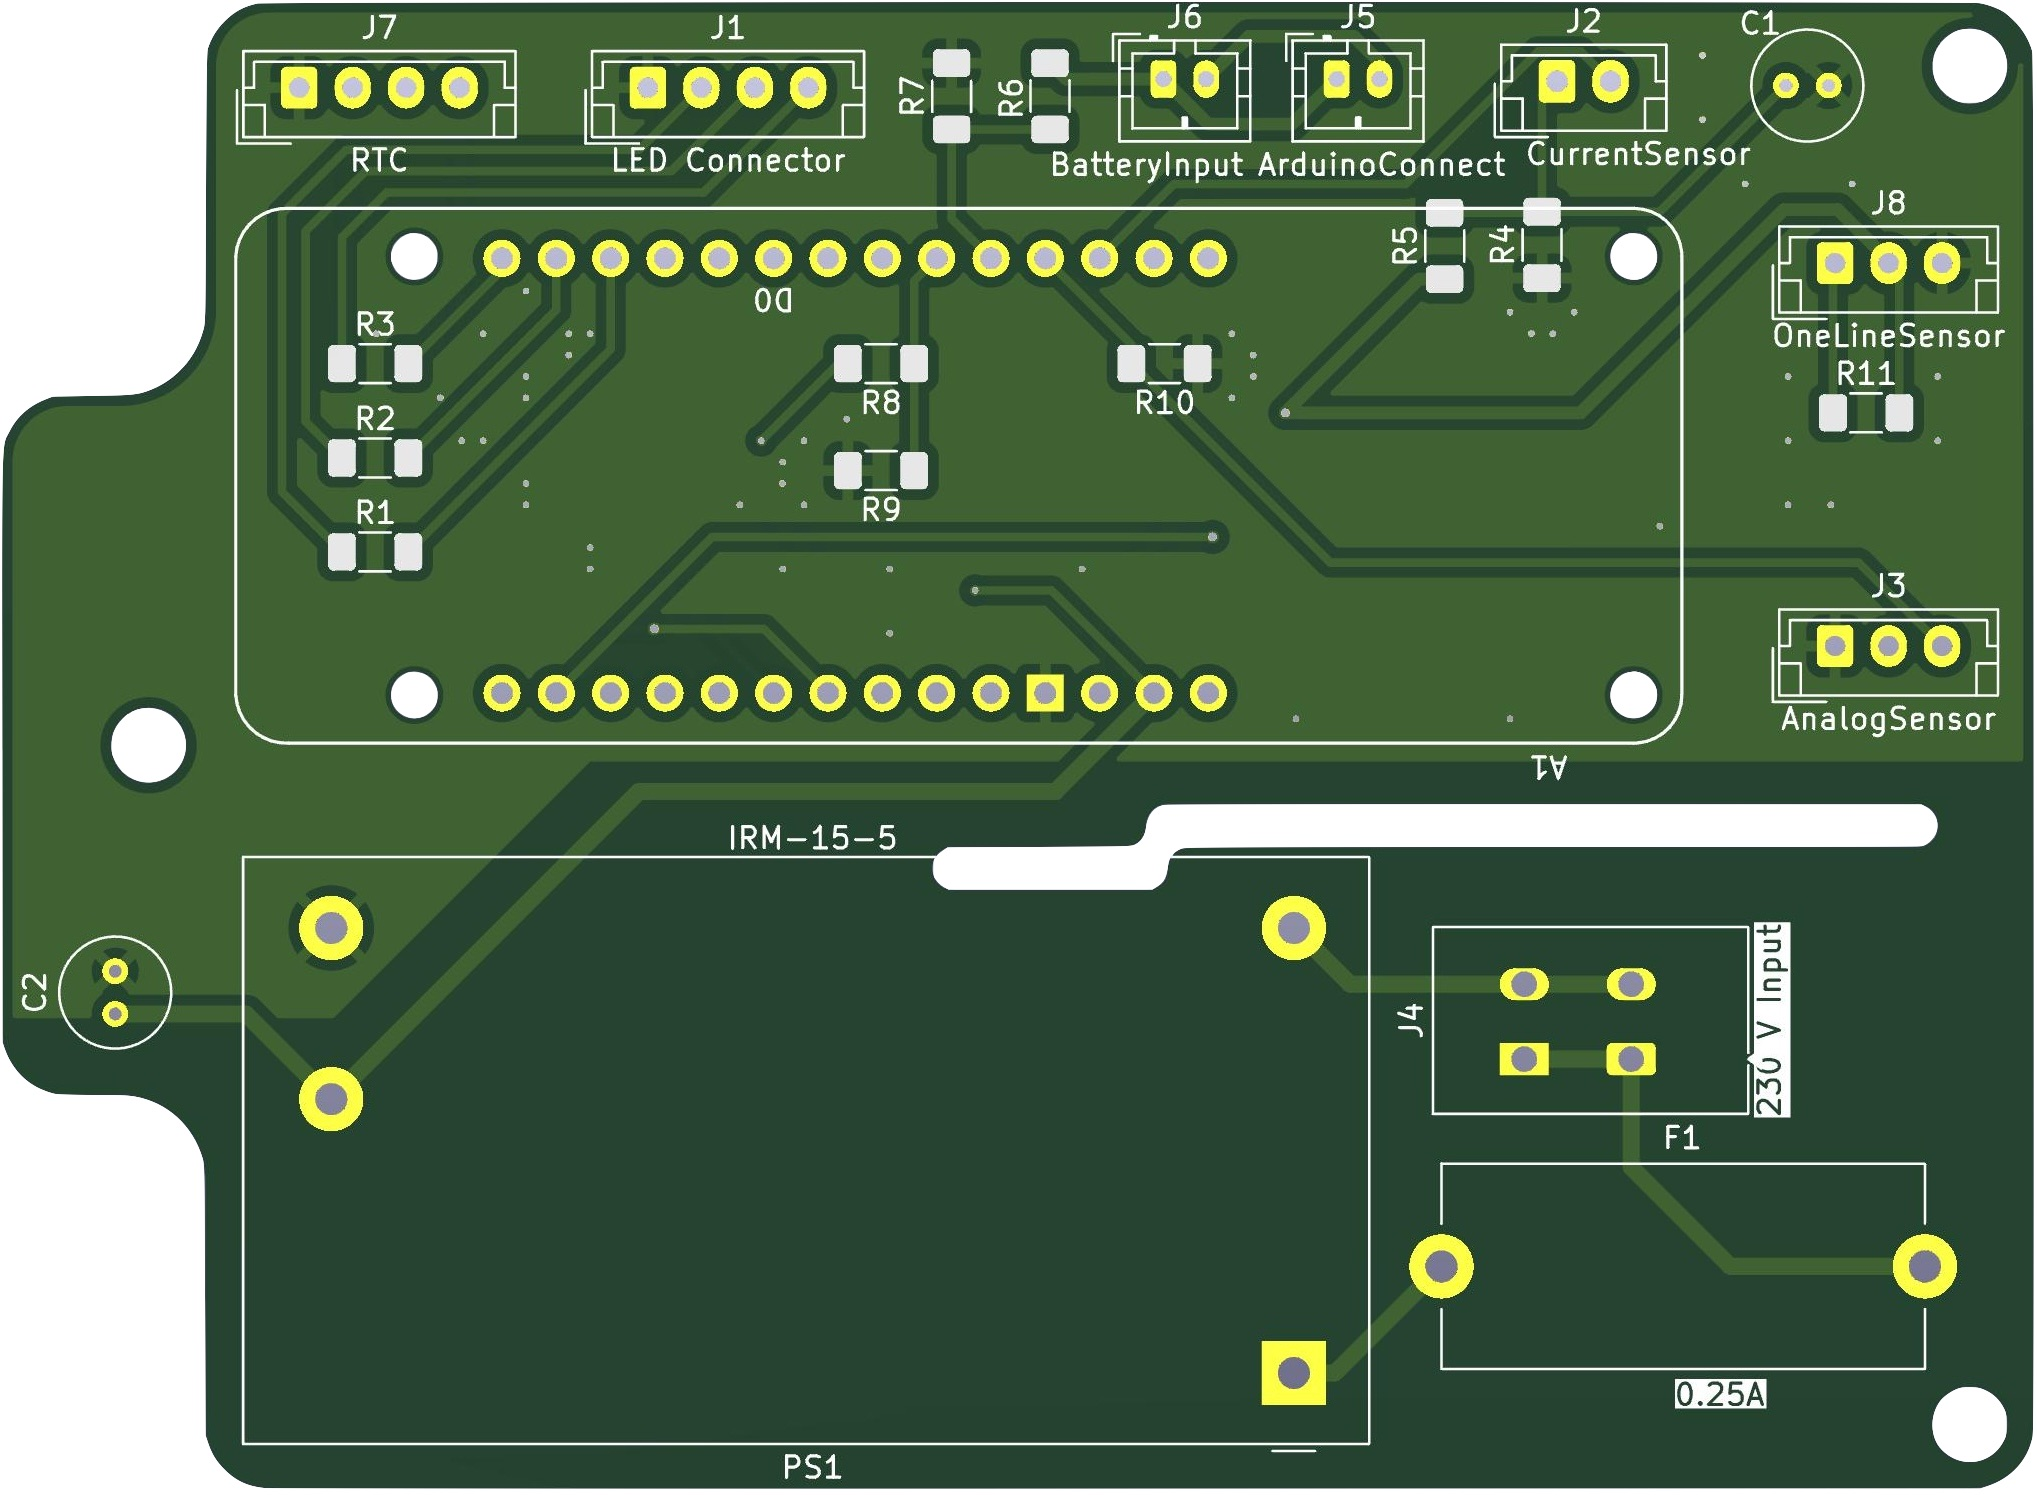
\includegraphics[width=5cm, angle=90]{Images/LoRaPCB/PCBforMKRWAN1310}};
	
	% ##########  	ANTENNA		###################
	\fill[yellow] (5.01,2) rectangle (5.4,2.3);
	\fill[black, rounded corners=2pt] (5.2,1.9) rectangle (5.9,2.4);
	\fill[black] (5.8,2.15) circle (0.25);
	
	% Vertical part
	\shade[inner color=black!40, outer color=black] (5.7,2.15) -- (5.7,5) -- (5.85,7) -- (5.95,7) -- (6.1,5) -- (6.1,2.15) -- (5.7,2.15);
	\fill[black] (5.95,2.15) circle (0.15);
	\fill[black] (5.9,7) circle (0.06);
	\draw[red, ->, thick, >=angle 60] (7.3, 3)  node[right] {\small\shortstack{Antenne}} -- (6.2, 3);	
	
	
}

\newcommand{\mainModuleSideView}{
	\shade[inner color=gray!30, outer color=gray!70, rounded corners=10pt] (0,0) rectangle (10, 4);
	
	% #########  CASE	################
	\draw[black, thick, rounded corners=10pt] (0,0) rectangle (10, 4);
	
	% LED
	\fill[white] (1.5, 2.8) circle (0.2 cm);
	\draw[red, ->, thick, >=angle 60] (- 0.5, 2.8)  node[left] {\small\shortstack{RGB Led}} -- (1.3, 2.8);	
	
	% Antenna Connector
	\fill[yellow] (1.5, 1.2) circle (0.3 cm);
	\draw[black] (1.5, 1.2) circle (0.2 cm);
	\fill[black] (1.5, 1.2) circle (0.05 cm);
	\draw[red, ->, thick, >=angle 60] (- 0.5, 1.2)  node[left] {\small\shortstack{Antennenbuchse}} -- (1.2, 1.2);
	
	% SWITCH
	\fill[black, rounded corners=0.1cm] (2.5, 0.8) rectangle ++(1.2, 0.8);
	
	\fill[black!60] (2.55, 0.85) rectangle (3.1, 1.55);
	\fill[black!80] (3.1, 0.85) rectangle (3.65, 1.55);
	
	\draw[white, thick, opacity=0.2] (3.1, 0.85) -- (3.1, 1.55);
	
	\node[white, font=\bfseries] at (2.825, 1.2) {O};
	\node[white, font=\bfseries] at (3.375, 1.2) {I};
	
	\draw[red, ->, thick, >=angle 60] (2.5, -0.5)  node[below] {\small\shortstack{Wippschalter}} -- (3.1, 0.7);
	% powering cables
	
	\fill[white!70] (6, 1)
	++(0:0.5cm)
	\foreach \a in {60,120,...,360} {
		-- ++(\a:0.5cm)
	} -- cycle;
	\draw[black] (6.25, 1.425) circle (0.3 cm);
	\draw[red, ->, thick, >=angle 60] (7, -0.5)  node[below] {\small\shortstack{Kabelführungen für die Sensoren}} -- (6.25, 0.9);
	
	\fill[white!70] (7.5, 1)
	++(0:0.5cm)
	\foreach \a in {60,120,...,360} {
		-- ++(\a:0.5cm)
	} -- cycle;
	\draw[black] (7.75, 1.425) circle (0.3 cm);
	\draw[red, ->, thick, >=angle 60] (7, -0.5) -- (7.75, 0.9);
}

\newcommand{\mainModuleInternal}{
	\shade[inner color=gray!30, outer color=gray!70, rounded corners=10pt] (0,0) rectangle (5, 10.5);
	
	% #########  CASE	################
	\draw[black, thick, rounded corners=10pt] (0,0) rectangle (5, 10.5);
	\draw[black, thick, rounded corners=10pt] (0.2,0.2) rectangle (4.8, 10.3);
	
	% PCB Board
	\node[anchor=south west, inner sep=0pt] at (1.2,5.2) {
\includegraphics[width=5cm, angle=270]{LoRaPCB/PCBforMKRWAN1310}};
	
	\ArduinoMkrWan{0.245}{0}{3.025}{7.7}{0}
	
	% ##########  	ANTENNA		###################
	\fill[yellow] (5.01,2) rectangle (5.4,2.3);
	\fill[black, rounded corners=2pt] (5.2,1.9) rectangle (5.9,2.4);
	\fill[black] (5.8,2.15) circle (0.25);
	
	% Vertical part
	\shade[inner color=black!40, outer color=black] (5.7,2.15) -- (5.7,5) -- (5.85,7) -- (5.95,7) -- (6.1,5) -- (6.1,2.15) -- (5.7,2.15);
	\fill[black] (5.95,2.15) circle (0.15);
	\fill[black] (5.9,7) circle (0.06);
	%\draw[red, ->, thick, >=angle 60] (7.3, 3)  node[right] {\small\shortstack{Antenne}} -- (6.2, 3);	
	
	
}

% #1 = scale
% #2 = angle
% #3 = x coordinate
% #4 = y coordinate
\newcommand{\temperatureSensorGeneral}[4]{
	% NodeNames
	%   ds18b20-VCC
	%   ds18b20-Signal
	%   ds18b20-GND
	\begin{scope}[shift={(#3, #4)}]
		\begin{scope}[scale=#1, rotate=#2]
			
			\draw[line width=#1*0.4cm, color=Gold] (0, 0) -- (2, 0);
			\draw[line width=#1*0.2cm, color=black] (2, 0) -- (6, 0);
			\draw[line width=#1*0.5cm, color=black] (2, 0) -- (2.4, 0);
			
			% Wires
			\node[inner sep=0pt, outer sep=0pt, minimum size=0pt, draw=none] (DS-WIRE) at (6,0) {};
			
			
			% connector
			%\foreach \xShift/\yShift in {7/-0.40} {
				%    \fill[brown!40] ($ (0, 0) + (\xShift,\yShift) $) rectangle ($ (0.8, 0.8) + (\xShift,\yShift) $);
				%    \fill[brown!20] ($ (0, -0.1) + (\xShift,\yShift) $) rectangle ($ (0.1, 0.9) + (\xShift,\yShift) $);
				%    \fill[brown!20] ($ (0.8, 0.5) + (\xShift,\yShift) $) rectangle ++(-0.4, -0.2);
				%}
			
			
		\end{scope}
	\end{scope}
}

\newcommand{\dsTempSensorBlockDiagramm}{
	
	
	\tikzset{
		line/.style={line width=0.25mm, >=stealth}
	}
	
	\ctikzset{
		resistors/scale=0.8,
		capacitors/scale=0.7,
		diodes/scale=0.6
	}
	
	\draw[black] (-0.5, 0) rectangle (15,8);
	\draw[black] (1.2, 0.3) rectangle (14.7,7.7);
	
	\node[draw,rectangle, minimum height=7cm, minimum width=3cm] (PPC) at (3.5,4){};
	
	\node[draw, rectangle, minimum height=7cm, minimum width=1cm, right=0.8cm of PPC] (ROM) {\small\shortstack{64-Bit\\ROM\\und\\1-Wire\\Port}};
	
	\node[draw, rectangle, minimum height=1cm, minimum width=2cm, anchor=north west] (MCL) at ([xshift=0.8cm]ROM.north east) {\small\shortstack{Speicher-\\Steuerlogik}};
	
	\node[draw, rectangle, minimum height=5cm, minimum width=2cm, anchor=south west] (SCRPAD) at ([xshift=0.8cm]ROM.south east) {\small\shortstack{Scratchpad}};
	
	\node[draw, rectangle, minimum height=0.7cm, minimum width=3.8cm, anchor=north west] (TEMPSEN) at ([xshift=0.8cm]SCRPAD.north east) {\small\shortstack{Temperatur-\\Register}};
	
	\node[draw, rectangle, minimum height=0.7cm, minimum width=3.8cm, below=0.12cm of TEMPSEN.south, anchor=north] (TH) {\small\shortstack{Alarm-Hochschwellen-\\Reg. ($T_H$) (EEPROM)}};
	
	\node[draw, rectangle, minimum height=0.7cm, minimum width=3.8cm, below=0.12cm of TH.south, anchor=north] (TL) {\small\shortstack{Alarm-Niedrigschwellen-\\Reg. ($T_L$) (EEPROM)}};
	
	\node[draw, rectangle, minimum height=0.7cm, minimum width=3.8cm, below=0.12cm of TL.south, anchor=north] (CONFREG) {\small\shortstack{Konfigurations-\\Register (EEPROM)}};
	
	\node[draw, rectangle, minimum height=0.7cm, minimum width=3.8cm, anchor=south west] (CRC) at ([xshift=0.8cm]SCRPAD.south east) {\small\shortstack{8-Bit CRC-Generator}};
	
	\draw[line, ->] (TEMPSEN.west) -- (SCRPAD.east |- TEMPSEN.west);
	\draw[line, <->] (TH.west) -- (SCRPAD.east |- TH.west);
	\draw[line, <->] (TL.west) -- (SCRPAD.east |- TL.west);
	\draw[line, <->] (CONFREG.west) -- (SCRPAD.east |- CONFREG.west);
	\draw[line, <->] (CRC.west) -- (SCRPAD.east |- CRC.west);
	
	\draw[line, ->] (MCL.south) -- (SCRPAD.north -| MCL.south);
	\draw[line, <->] (MCL.west) -- (ROM.east |- MCL.west);
	
	% circuit
	\draw[line, <-] ([yshift=-2.0cm]ROM.north west) -- ++(-5.5, 0) coordinate(startPunktUp);
	\draw[line, <-] ([yshift=2.0cm]ROM.south west) -- ([yshift=2.0cm]ROM.south west -| startPunktUp) coordinate(startPunktDown);
	
	\node[anchor=south west] at ([xshift=-0.2cm]startPunktDown) {\small{$V_{DD}$}};
	\node[anchor=north west] at ([xshift=-0.2cm]startPunktUp) {\small{$D_Q$}};
	\node[anchor=south west] at ([xshift=-0.2cm]$(startPunktUp)!0.5!(startPunktDown)$) {\small{GND}};
	
	\draw[line] ($(startPunktUp)!0.5!(startPunktDown)$) -- ++(1.3,0) -- ++(0,-0.25) node[sground]{};
	
	\draw[line] ($(startPunktUp)+(0.5, 0)$) to[R, l=\(R_{{4.7}k\Omega}\)] ++(0,1.7) node[rground, rotate=180, label={[xshift=-1mm, yshift=4mm]left:$V_{PU}$}]{};
	\fill[black] ($(startPunktUp)+(0.5, 0)$) circle (0.07cm);
	
	\coordinate (mid) at ($(startPunktUp)!0.5!(startPunktDown)$);
	\draw[line, ->] ($(mid)+(3.2,0)$) coordinate(startPunkMid) -- (ROM.west);
	
	\fill[black] (startPunkMid) circle (0.07cm);
	
	\draw[line] (startPunkMid) -| ++(-0.7, -0.1) to[C, l_=$C_{pp}$] ++(0,-0.5) coordinate (A);
	
	
	\draw[line] (A) node[sground]{};
	
	\draw[line, ->] (startPunkMid |- startPunktDown) to[diode, fill=black] (startPunkMid);
	
	\draw[line, ->] (startPunkMid |- startPunktUp) to[diode, fill=black] (startPunkMid);
	
	\fill[black] (startPunkMid |- startPunktDown) circle (0.07cm);
	\fill[black] (startPunkMid |- startPunktUp) circle (0.07cm);
}


\newcommand{\dsTempRegisterFormat}{
	
	\foreach \x in {0,...,7} {
		\foreach \y in {0, -1.5} {
			\draw[black] ({\x-0.5},{\y-0.25}) rectangle ({\x+0.5},{\y+0.25});
		}
	}
	
	\foreach \x in {0,...,7}{
		\pgfmathsetmacro{\bit}{int(7-\x)}
		\pgfmathsetmacro{\exponent}{int(3-\x)}
		\node[] at (\x, 0.5){\scriptsize{Bit \bit}};
		
		\node[] at (\x, 0.0){\scriptsize{$2^{\exponent}$}};
	}
	
	\foreach \x in {0,...,7}{
		\pgfmathsetmacro{\bit}{int(15-\x)}
		\node[] at (\x, -1){\scriptsize{Bit \bit}};
	}
	
	\foreach \x in {0,...,2}{
		\pgfmathsetmacro{\exponent}{int(6-\x)}
		\node[] at ({\x+5}, -1.5){\scriptsize{$2^{\exponent}$}};
	}
	
	\foreach \x in {0,...,4}{
		\node[] at (\x, -1.5){\scriptsize{S}};
	}
	
	\node[] at (-1.2, 0) {\scriptsize{LS-Byte}};
	\node[] at (-1.2, -1.5) {\scriptsize{MS-Byte}};
	\node[] at (-1.0, -2.5) {\scriptsize{S = Vorzeichen}};
}

\newcommand{\dsAlarmRegisterFormat}{
	\pgfmathsetmacro{\y}{0}
	\foreach \x in {0,...,7} {
		\draw[black] ({\x-0.5},{\y-0.25}) rectangle ({\x+0.5},{\y+0.25});
		
	}
	
	\foreach \x in {0,...,7}{
		\pgfmathsetmacro{\bit}{int(7-\x)}
		\node[] at (\x, 0.5){\scriptsize{Bit \bit}};
	}
	
	\foreach \x in {1,...,7}{
		\pgfmathsetmacro{\exponent}{int(7-\x)}
		\node[] at (\x, 0.0){\scriptsize{$2^{\exponent}$}};
	}
	\node[] at (0, 0) {\scriptsize{S}};
}

\newcommand{\dsConfigRegisterFormat}{
	\pgfmathsetmacro{\y}{0}
	\foreach \x in {0,...,7} {
		\draw[black] ({\x-0.5},{\y-0.25}) rectangle ({\x+0.5},{\y+0.25});
		
	}
	
	\foreach \x in {0,...,7}{
		\pgfmathsetmacro{\bit}{int(7-\x)}
		\node[] at (\x, 0.5){\scriptsize{Bit \bit}};
	}
	
	\foreach \x in {3,...,7}{
		\node[] at (\x, 0.0){\scriptsize{1}};
	}
	\node[] at (0, 0) {\scriptsize{0}};
	\node[] at (1, 0) {\scriptsize{R1}};
	\node[] at (2, 0) {\scriptsize{R0}};
}

\newcommand{\dsLaseredRomCode}{
	\node[draw, rectangle, minimum width=4cm, minimum height=1cm] (CRC) {8-Bit CRC};
	\node[draw, rectangle, minimum width=5cm, minimum height=1cm, anchor=west] at (CRC.east) (SERNUM) {48-Bit Seriennummer};
	\node[draw, rectangle, minimum width=4cm, minimum height=1cm, anchor=west] at (SERNUM.east) (FAMNUM) {8-Bit Family Code (28h)};
	
	\foreach \i in {CRC, SERNUM, FAMNUM} {
		\node[anchor=north west] at ([xshift=0.2cm]\i.south west) {MSB};
		\node[anchor=north east] at ([xshift=-0.2cm]\i.south east) {LSB};
	}
}


\newcommand{\dsMemoryMap}{
	\tikzset{
		line/.style={line width=0.1cm, >=stealth}
	}
	
	% scratchpad nodes
	\node[draw, rectangle, minimum width=6cm, minimum height=1cm] (TEMPLSB) {Temperatur-LSB};
	
	\node[draw, rectangle, minimum width=6cm, minimum height=1cm, anchor=north] (TEMPMSB) at (TEMPLSB.south) {Temperatur-MSB};
	
	\node[draw, rectangle, minimum width=6cm, minimum height=1cm, anchor=north] (TH) at (TEMPMSB.south) {$T_H$-Register oder Benutzer-Byte 1};
	
	\node[draw, rectangle, minimum width=6cm, minimum height=1cm, anchor=north] (TL) at (TH.south) {$T_L$-Register oder Benutzer-Byte 2};
	
	\node[draw, rectangle, minimum width=6cm, minimum height=1cm, anchor=north] (CONFIGREG) at (TL.south) {Konfigurations-Register};
	
	\node[draw, rectangle, minimum width=6cm, minimum height=1cm, anchor=north] (RES1) at (CONFIGREG.south) {Reserviertes Register};
	
	\node[draw, rectangle, minimum width=6cm, minimum height=1cm, anchor=north] (RES2) at (RES1.south) {Reserviertes Register};
	
	\node[draw, rectangle, minimum width=6cm, minimum height=1cm, anchor=north] (RES3) at (RES2.south) {Reserviertes Register};
	
	\node[draw, rectangle, minimum width=6cm, minimum height=1cm, anchor=north] (CRC) at (RES3.south) {CRC-Register};
	
	% eeprom nodes
	\node[draw, rectangle, minimum width=6cm, minimum height=1cm, anchor=west] (THEPROM) at ([xshift=2cm]TH.east) {$T_H$-Register oder Benutzer-Byte 1};
	
	\node[draw, rectangle, minimum width=6cm, minimum height=1cm, anchor=west] (TLEPROM) at ([xshift=2cm]TL.east) {$T_L$-Register oder Benutzer-Byte 2};
	
	\node[draw, rectangle, minimum width=6cm, minimum height=1cm, anchor=west] (CONFEPROM) at ([xshift=2cm]CONFIGREG.east) {Konfigurations-Register};
	
	% names
	\node[anchor=south] at ([yshift=0.2cm]TEMPLSB.north) {\large{\textbf{Scratchpad}}};
	
	\node[anchor=south] at ([yshift=0.2cm]THEPROM.north) {\large{\textbf{EEPROM}}};
	
	
	\draw[line, <->] (TH) -- (THEPROM);
	\draw[line, <->] (TL) -- (TLEPROM);
	\draw[line, <->] (CONFIGREG) -- (CONFEPROM);
	
	\newcounter{bytenum}
	\setcounter{bytenum}{0}
	\foreach \i in {TEMPLSB, TEMPMSB, TH, TL, CONFIGREG, RES1, RES2, RES3, CRC} {
		\node[anchor=east] at ([xshift=-0.5cm]\i.west) {Byte \thebytenum};
		\addtocounter{bytenum}{1}
	}
}


% #1 = scale
% #2 = angle
% #3 = x coordinate
% #4 = y coordinate
% coordinate for the cable: SCT-WIRE
\newcommand{\sctGeneral}[4]{
	\begin{scope}[shift={(#3, #4)}]
		\tikzset{
			lineScaled/.style n args={1}			{line width={#1*3pt}},
			lineScaledWire/.style n args={1}		{line width={#1*20pt}},
			cornersScaled/.style n args = {1}	    {rounded corners={#1*15pt}},
			cornersScaledSmall/.style n args = {1}	{rounded corners={#1*10pt}},
			cornersScaledBig/.style n args = {1}	{rounded corners={#1*60pt}},
		}
		\begin{scope}[scale=#1, rotate=#2]
			
			% Grid for the picture
			
			%\foreach \x in {-5,...,5} {
				%	\fill[red] (\x, -8) circle (0.2);
				%	\node[red] at (\x, -8.8) {\Large \x};
				
				%	\fill[red] (\x, 8) circle (0.2);
				%	\node[above, red] at (\x, 8.8) {\Large \x};
				%}
			
			%\foreach \y in {-10,...,10} {
				%	\fill[red] (-5.5, \y) circle (0.2);
				%	\node[left, red] at (-6.2, \y) {\Large \y};
				%}
			
			
			
			% blue layout
			\fill[blue, cornersScaled] (0, 7.7) -- (4.1, 7.7) -- (4.1, -7.7) -- (-2, -7.7) -- (-2, -2.8) -- (-3.8, -2.8)[sharp corners] -- (-3.8, 2.5) -- (-4.5, 2.5)[cornersScaled] -- (-4.5, 7.7) -- cycle;
			\fill[blue] (-4.5, 2.5) -- (-4.5, -2) -- ++(-0.4, -0.4) -- ++(0.25, -0.25) -- ++(0.50, 0.5) |- (-4.5, 2.5);
			\fill[blue] (4.0, 3) -- (4.6, 2.5) -- (4.0, 2) -- cycle;
			
			% white infill
			\fill[cornersScaledSmall, white] (-1.8, 2.5) -- (-1.8, 5) -- (2, 5)-- (2, 1.3) -- (-1.8, 1.3) -- cycle;
			% gray coil
			\fill[gray!80] (-1.8, 3.5)[cornersScaledBig] -- (0.1, 5.2)[sharp corners] -- (2, 3.5)[cornersScaledSmall] -- (2, 5) -- (-1.8, 5)[sharp corners] -- cycle;
			
			% black separator line
			\draw[lineScaled, black] (-3.8, 2.5) -- (-1.8, 2.5);
			\draw[lineScaled, black] (2, 2.5) -- (4.5, 2.5);
			\filldraw[gray] (4.35, 2.5) circle (0.08cm);
			
			% cable
			
			\draw[black, lineScaledWire] (0.5, -7.7) -- ++(0, -2) node[inner sep=0pt, outer sep=0pt, minimum size=0pt, draw=none] (SCT-WIRE) {};;
			
			% Background template picture -> edit in scale 1
			%\node[anchor=center, inner sep=0pt, opacity=0.3] at (0,0) {\includegraphics[width=10cm, angle=0]{../Images/Sensor/SCT013/SCT013.png}};
		\end{scope}
	\end{scope}
}

% #1 = x min
% #2 = x max
% #3 = y min
% #4 = y max
\newcommand{\draftGrid}[4]{
	% Grid for the picture
	
	\foreach \x in {#1,...,#2} {
		\fill[red] (\x, #3) circle (0.2);
		\node[red] at (\x, {#3 - 0.8}) {\Large \x};
		
		\fill[red] (\x, #4) circle (0.2);
		\node[above, red] at (\x, {#4 + 0.8}) {\Large \x};
	}
	
	\foreach \y in {#3,...,#4} {
		\fill[red] (#1, \y) circle (0.2);
		\node[left, red] at ({#1 - 0.7}, \y) {\Large \y};
	}
}


\newcommand{\workingPrinciple}[4]{
	\begin{scope}[shift={(#3, #4)}]
		\tikzset{
			lineScaled/.style n args={1}			        {line width={#1*1pt}},
			lineScaledSecondarySide/.style n args={1}		{line width={#1*2pt}},
			lineScaledWire/.style n args={1}		        {line width={#1*9pt}},
			arrowStyle/.style=                              {lineScaledSecondarySide, >=stealth},
			labelnode/.style n args={1}                     {scale=#1*1.0}
		}
		\begin{scope}[scale=#1, rotate=#2]
			
			%\draftGrid{-7}{6}{-4}{4}
			
			% coil
			\fill[gray!20] (-3.85, 2.25) -- ++(0.4, 0.4) -- ++(5.25, 0) -- ++(0, -5.15) -- ++(-0.4, -0.4) -- ++(-5.25, 0) -- cycle;
			\draw[gray, lineScaled] (-3.85, 2.25) -- ++(5.25, 0) coordinate(A) -- ++(0, -5.15) coordinate (C) -- ++(-5.25, 0) -- cycle;
			\draw[gray, lineScaled] (-3.85, 2.25) -- ++(0.4, 0.4) -- ++(5.25, 0) coordinate(B) -- (A);
			\draw[gray, lineScaled] (B) -- ++(0, -5.15) -- (C);
			\draw[black, arrowStyle, <-] (1, 2) -- ++(2, 1) node[right, labelnode] {Ferritkern};
			
			% space inside coil
			\draw[gray, lineScaled, fill=gray!60] (0.2, 0.75) rectangle ++(-2.7, -2.15) coordinate(R1);
			\draw[gray, lineScaled, fill=white] (0.2, 0.75) rectangle ++(-2.45, -1.80) coordinate(R2);
			\draw [gray, lineScaled] (R1) -- (R2);
			
			% Primary side wires
			\draw[blue, lineScaledWire] (-6, 3) node[black, above, labelnode]{N} -- (-6, -4);
			\draw[brown, lineScaledWire] (-5,3) node[black, above, labelnode]{L} -- (-5,1.5) arc[start angle=180, end angle=270, radius=#1*1cm] -- (-2,0.5) arc[start angle=90, end angle=-90, radius=#1*0.6cm] (-2, -0.7) -- ++(-0.235, 0);
			\draw[orange!40!red, arrowStyle, ->] (-4.7, 2.8) -- node[black, midway, right, labelnode] {$I_{p}$} (-4.7, 1.5);
			\draw[orange!40!red, arrowStyle, ->] (-4.7, -2) -- node[black, midway, right, labelnode] {$I_{p}$} (-4.7, -4);
			
			\draw[brown, lineScaledWire] (-3.86, -0.7) -- (-4, -0.7) arc[start angle=90, end angle=180, radius=#1*1cm] -- (-5, -4);
			
			\draw[black, lineScaledSecondarySide] (0.2, -1.35) -- (4.5, -1.35);
			\draw[black, lineScaledSecondarySide] (1.8, 0.55) -- (4.5, 0.55);
			\draw[black,lineScaledSecondarySide, fill=white] (4.5, -1.35) circle (0.1cm);
			\draw[black,lineScaledSecondarySide, fill=white] (4.5, 0.55) circle (0.1cm);
			
			\draw[black, arrowStyle, ->] (4.5, -1.15) -- node[midway, right, labelnode] {$U_s$} (4.5, 0.35);
			
			% Burden resistor
			\fill[black] (2.6, -1.35) circle (0.1cm);
			\fill[black] (2.6, 0.55) circle (0.1cm);
			\draw[black, lineScaledSecondarySide] (2.6, -1.35) -- ++ (0, 0.5);
			\draw[black, lineScaledSecondarySide] (2.6, 0.55) -- ++ (0, -0.5);
			\draw[black, lineScaledSecondarySide] (2.4, -0.85) rectangle (2.8, 0.05);
			
			\draw[orange!40!red, arrowStyle, ->] (3, 0.55) -- node[black, midway, above]
			{\Large{$I_{s}$}} (4.2, 0.55);
			
			\draw[black, arrowStyle, <-] (2.85, -0.9) -- ++(1, -1.5) node[below, labelnode] {\shortstack{Belastungs-\\widerstand}};
			\node[labelnode] at (3.05, -0.5) {$R_b$};
			
			
			% Wirings
			\foreach \y in {-1.0, -0.65, -0.3, 0.05, 0.4} {
				\draw[black, lineScaledSecondarySide] (0.2, \y) -- (1.3, {\y-0.15}) to[out=-10, in=190] (1.55, {\y-0.15}) -- (1.95, {\y-0.1}) to [out=35, in=0] (1.8, {\y});
				%\draw[black, lineScaledSecondarySide] (1.55, {\y+0.05}) -- (1.9, {\y+0.4});
				\draw[black, lineScaledSecondarySide] (0.2, \y) arc[start angle=270, end angle=90, x radius=0.1cm, y radius=0.07cm];
			}
			\draw[black, lineScaledSecondarySide] (0.2, -1.35) arc[start angle=270, end angle=90, x radius=0.1cm, y radius=0.07cm];
			
			%
			\draw[red, arrowStyle, <-] (-2, -1) -- ++(-0.9, -3) node[below, labelnode] {Primärwicklung};
			\draw[red, arrowStyle, <-] (1, -1.4) -- ++(0.9, -2.6) node[below, labelnode] {Sekundärwicklung};
			
		\end{scope}
	\end{scope}
	
}

% INTERN-ANT
\newcommand{\mikrotikInside}{
	\mikrotikInsideEnclosure{0.7}{0}{0}{0}
	\mikrotikGatewayTopEnclosure{0.7}{0}{0}{0}
	\routerPlatform{0.7}{90}{0}{2.5}
	\loraCard{0.7}{90}{0}{2.5}
	
	\fill[green!70!black] (3.5, 5.1) -- ++(-0.5, 0) -- ++(0, -10) -- ++(0.5, 0.2) -- cycle;
	\coordinate (INTERN-ANT) at (3.25, 5.1);
	
}

\newcommand{\mikrotikInsideEnclosure}[4]{
	\begin{scope}[shift={(#3, #4)}]
		\begin{scope}[scale=#1, rotate=#2]	
			\tikzset{
				lineScaled/.style n args={1}			{line width={#1*5pt}},
				cornersScaled/.style n args = {1}	    {rounded corners={#1*2pt}},
				rectangleScaled/.style n args={1}    {rounded corners={#1*40pt}},
				rectangleScaledInner/.style n args={1}    {rounded corners={#1*30pt}},
			}
			
			
			\fill[gray!20] (-4.5, -1.5) -- (4.5, -1.5)[rectangleScaledInner] -- (4.5, 9.5) -- (-4.5, 9.5)[sharp corners] -- cycle;
			\fill[gray!10] (-4.5, -1.5)[rectangleScaledInner] -- (-4.5, -9) -- (4.5, -9)[sharp corners] -- (4.5, -1.5) -- cycle;
			
			\fill[Gold] (1, -1.5) rectangle ++(1, -0.25);
			\fill[Gold] (1.25, -1.75) rectangle ++(0.5, -0.8);
			\coordinate(SMA-INPUT) at (1.5, -1.5);
			\coordinate(SMA-OUTPUT) at (1.5, -2.5);
			%\fill[gray!10, rectangleScaled](-5, -10) rectangle (5, 10);
			%\fill[gray!20, rectangleScaledInner](-4.5, -9.5) rectangle (4.5, 9.5);
			
			\draw[lineScaled, gray!50] (-4.5, -1.5) -- (4.5, -1.5);
		\end{scope}
	\end{scope}
}
% SMA-INPUT
% SMA-OUTPUT
\newcommand{\mikrotikGatewayTopEnclosure}[4]{
	\begin{scope}[shift={(#3, #4)}]
		\begin{scope}[scale=#1, rotate=#2]	
			\tikzset{
				lineScaled/.style n args={1}			{line width={#1*2pt}},
				cornersScaled/.style n args = {1}	    {rounded corners={#1*2pt}},
				rectangleScaled/.style n args={1}    {rounded corners={#1*40pt}},
				rectangleScaledInner/.style n args={1}    {rounded corners={#1*30pt}},
			}
			
			\fill[gray!10] (-5, -1.5) -- (5, -1.5)[rectangleScaled] -- (5, 10) -- (-5, 10)[sharp corners] -- cycle;
			\fill[gray!20] (-4.5, -1.5) -- (4.5, -1.5)[rectangleScaledInner] -- (4.5, 9.5) -- (-4.5, 9.5)[sharp corners] -- cycle;
			%\fill[gray!10] (-4.5, -1.5)[rectangleScaledInner] -- (-4.5, -9) -- (4.5, -9)[sharp corners] -- (4.5, -1.5) -- cycle;
			\draw[lineScaled, gray!50] (-4.5, -1.5) -- (4.5, -1.5);
		\end{scope}
	\end{scope}
}

\newcommand{\mikrotikGatewayBottomEnclosure}[4]{
	\begin{scope}[shift={(#3, #4)}]
		\begin{scope}[scale=#1, rotate=#2]	
			\tikzset{
				rectangleScaled/.style n args={1}    {rounded corners={#1*40pt}},
				rectangleScaledInner/.style n args={1}    {rounded corners={#1*30pt}},
			}
			
			\fill[gray!10] (-5, -1.5)[rectangleScaled] -- (-5, -10) -- (5, -10)[sharp corners] -- (5, -1.5) -- cycle;
			\fill[gray!20] (-4.5, -1.5)[rectangleScaledInner] -- (-4.5, -9.5) -- (4.5, -9.5)[sharp corners] -- (4.5, -1.5) -- cycle;
		\end{scope}
	\end{scope}
	
}

\newcommand{\routerPlatform}[4]{
	\begin{scope}[shift={(#3, #4)}]
		\tikzset{
			lineScaled/.style n args={1}			{line width={#1*3pt}},
			lineScaledWire/.style n args={1}		{line width={#1*20pt}},
			cornersScaled/.style n args = {1}	    {rounded corners={#1*15pt}},
			cornersScaledSmall/.style n args = {1}	{rounded corners={#1*10pt}},
			cornersScaledBig/.style n args = {1}	{rounded corners={#1*60pt}},
		}
		\begin{scope}[scale=#1, rotate=#2]
			
			% Grid for the picture
			
			%\foreach \x in {-5,...,5} {
				%	\fill[red] (\x, 4) circle (0.2);
				%	\node[red] at (\x, -4.8) {\Large \x};
				
				%	\fill[red] (\x, -4) circle (0.2);
				%	\node[above, red] at (\x, 4.8) {\Large \x};
				%}
			
			%\foreach \y in {-4,...,4} {
				%	\fill[red] (-5.5, \y) circle (0.2);
				%	\node[left, red] at (-6.2, \y) {\Large \y};
				%}
			
			\fill[ArduinoColor] (-5, -3.7) rectangle (5, 3.7);
			
			
			
			\fill[black] (-2.75, -2.4) circle (13pt);
			\fill[black] (-2.75, 2.8) circle (13pt);
			
			%capacitor
			\fill[yellow] (-2.65, 0.75) circle (15pt);
			\fill[gray!30] (-2.65, 0.75) circle (11pt);
			
			\fill[gray!30] (1.4, 1) circle (6pt);
			
			% heat sink
			\begin{scope}[shift={(2.4, 0)}]
				\pgfmathsetmacro{\i}{0.8}
				\begin{scope}[rotate=-45]
					\fill[black!70](-\i, -\i) rectangle (\i, \i);
					
					\foreach \x in {-\i*0.7, -\i*0.25, \i*0.25, \i*0.7} {
						\foreach \y in {-\i*0.7, -\i*0.25, \i*0.25, \i*0.7} {
							\fill[black] ({\x-0.15}, {\y-0.05}) rectangle ({\x+0.15}, {\y+0.05});
						}
					}
				\end{scope}
			\end{scope}
			
			
			\SMDTransistorAuto{0.6}{0}{-0.55}{2.9}{1}{0.6}{6}{6}{0.1}
			\SMDTransistorAuto{0.25}{-45}{1.7}{2}{1}{0.6}{3}{1}{0.3}
			\SMDTransistorAuto{0.25}{0}{-2.25}{-1.3}{1}{0.8}{3}{3}{0.3}
			\SMDTransistorAuto{0.15}{45}{3}{-2}{1}{0.6}{3}{3}{0.3}
			\SMDTransistorAuto{0.15}{-45}{3.6}{-1.4}{1}{0.6}{3}{3}{0.3}
			
			%Antenna Connector
			\begin{scope}[shift={(4.3, -1.2)}]
				\begin{scope}[scale=0.3, rotate=45, line width=0.03cm*#1]
					\fill[gray] (-0.6, 0.3) rectangle ++(1.2, 1.2);
					\fill[Gold] (0, 0.9) circle (0.12cm);
					\draw[Gold] (0, 0.9) circle (0.45cm);
				\end{scope}
			\end{scope}
			
			\begin{scope}[shift={(3.4, -2.7)}]
				\begin{scope}[scale=0.3, rotate=30, line width=0.03cm*#1]
					\fill[gray] (-0.6, 0.3) rectangle ++(1.2, 1.2);
					\fill[Gold] (0, 0.9) circle (0.12cm);
					\draw[Gold] (0, 0.9) circle (0.45cm);
				\end{scope}
			\end{scope}
			
			\foreach \y in {-2.55, -2.35} {
				\foreach \i in {0,...,5} {
					\pgfmathsetmacro{\x}{1.175 + \i*0.17}
					\draw[Gold, line width=0.33mm*#1] (\x, \y) circle (0.06cm);
				}
			}
			
			\begin{scope}[shift={(2.25, -2.08)}]
				\begin{scope}[rotate=45]
					\foreach \y in {0, 0.25} {
						\foreach \i in {0,...,1} {
							\pgfmathsetmacro{\x}{\i*0.25}
							\draw[Gold, line width=0.43mm*#1] (\x, \y) circle (0.075cm);
						}
					}
				\end{scope}
			\end{scope}
			
			\begin{scope}[shift={(1.45, -1.1)}]
				\begin{scope}[rotate=-45]
					\fill[gray!30] (-0.1, -0.17) rectangle (0.1, 0.17);
				\end{scope}
			\end{scope}
			
			\smallSMDCapacitor{0.06}{-45}{1.3}{-0.9}{ArduinoColor}
			\smallSMDCapacitor{0.08}{-45}{1.2}{2.6}{ArduinoColor}
			\smallSMDCapacitor{0.08}{90}{1.7}{2.6}{ArduinoColor}
			\smallSMDCapacitor{0.08}{-45}{1.5}{2.3}{ArduinoColor}
			\smallSMDCapacitor{0.08}{-45}{3}{3}{ArduinoColor}
			\smallSMDCapacitor{0.08}{45}{1.4}{1.7}{ArduinoColor}
			\smallSMDCapacitor{0.08}{-45}{2.5}{1.6}{ArduinoColor}
			\smallSMDCapacitor{0.1}{0}{0.3}{3.1}{ArduinoColor}
			\smallSMDCapacitor{0.1}{0}{-1.5}{3.1}{ArduinoColor}
			\smallSMDCapacitor{0.08}{90}{-2}{2.6}{ArduinoColor}
			\smallSMDCapacitor{0.08}{90}{-2}{2.8}{ArduinoColor}
			\smallSMDCapacitor{0.08}{0}{-2.3}{2.1}{ArduinoColor}
			\smallSMDCapacitor{0.08}{0}{-3.5}{-1.9}{ArduinoColor}
			\smallSMDCapacitor{0.08}{0}{-3.3}{-1.9}{ArduinoColor}
			\smallSMDCapacitor{0.04}{0}{-3.1}{-1.9}{ArduinoColor}
			\smallSMDCapacitor{0.08}{0}{-3.1}{-1.6}{ArduinoColor}
			\smallSMDCapacitor{0.08}{0}{-2.85}{-1.6}{ArduinoColor}
			\smallSMDCapacitor{0.04}{-45}{-2.3}{-1.9}{ArduinoColor}
			\smallSMDCapacitor{0.08}{0}{-3.5}{-2.8}{ArduinoColor}
			\smallSMDCapacitor{0.08}{0}{-3.75}{-2.8}{ArduinoColor}
			\smallSMDCapacitor{0.08}{0}{-2.35}{-0.7}{ArduinoColor}
			\smallSMDCapacitor{0.04}{0}{-2.2}{-0.7}{ArduinoColor}
			\smallSMDCapacitor{0.04}{0}{-2.2}{-0.7}{ArduinoColor}
			\smallSMDCapacitor{0.04}{0}{-2.1}{-0.65}{ArduinoColor}
			\smallSMDCapacitor{0.08}{-45}{1.7}{1.3}{ArduinoColor}
			
			\fill[gray!30] (-4.2, -2.5) rectangle ++(0.2, 0.3);
			\fill[gray!30] (-3.6, -2.5) rectangle ++(0.2, 0.3);
			
			\fill[gray!30] (1.3, 2.9) rectangle ++(0.25, 0.4);
			\fill[gray!30] (1.9, 2.9) rectangle ++(0.25, 0.4);
			
			\fill[black] (-2.5, -0.4) rectangle ++(0.25, 0.5);
			\fill[gray!30] (-2.45, -0.4) rectangle ++(0.15, -0.05);
			\fill[gray!30] (-2.45, 0.1) rectangle ++(0.15, 0.05);
			
			
			\begin{scope}[shift={(2.3, 1.3)}]
				\begin{scope}[rotate=-45]
					\foreach \y in {0, 0.13} {
						\foreach \i in {0,...,6} {
							\pgfmathsetmacro{\x}{\i*0.13}
							\smallSMDResistor{0.02}{0}{\x}{\y}{ArduinoColor}
						}
					}
				\end{scope}
			\end{scope}
			
			\begin{scope}[shift={(2.7, 1.5)}]
				\begin{scope}[rotate=-45]
					\foreach \y in {0} {
						\foreach \i in {0,...,4} {
							\pgfmathsetmacro{\x}{\i*0.18}
							\smallSMDResistor{0.04}{0}{\x}{\y}{ArduinoColor}
						}
					}
				\end{scope}
			\end{scope}
			
			\begin{scope}[shift={(3.2, 2.9)}]
				\begin{scope}[rotate=-45]
					\foreach \y in {0} {
						\foreach \i in {0,...,2} {
							\pgfmathsetmacro{\x}{\i*0.18}
							\smallSMDResistor{0.04}{0}{\x}{\y}{ArduinoColor}
						}
					}
				\end{scope}
			\end{scope}
			
			\begin{scope}[shift={(1.3, -2.2)}]
				\begin{scope}[rotate=0]
					\foreach \y in {0, 0.15} {
						\foreach \i in {0,...,3} {
							\pgfmathsetmacro{\x}{\i*0.2}
							\smallSMDResistor{0.04}{90}{\x}{\y}{ArduinoColor}
						}
					}
				\end{scope}
			\end{scope}
			
			\begin{scope}[shift={(1.1, -0.4)}]
				\begin{scope}[rotate=-45]
					\foreach \y in {0} {
						\foreach \i in {0,...,3} {
							\pgfmathsetmacro{\x}{\i*0.12}
							\smallSMDCapacitor{0.025}{0}{\x}{\y}{ArduinoColor}
						}
					}
				\end{scope}
			\end{scope}
			
			% drills
			\foreach \x/\y in {1.5/-3.25, 4.5/-2.7, 0.7/3.2} {
				\fill[white] (\x, \y) circle (1.5mm);
				\draw[Gold, line width=0.9mm*#1] (\x, \y) circle (1.6mm);
			}
			
			% reset button
			\fill[brown!30] (-4.6, -2.8) rectangle ++(0.3, 0.7);
			\fill[black] (-4.6, -2.6) rectangle ++(-0.1, 0.35);
			
			
			% LAN RJ45
			\fill[gray] (-4.5, 2) rectangle ++(1, 1.5);
			
			%Molex
			\fill[black] (-4.5, 0.7) rectangle ++(1.2, );
			
			% DC Connector
			\fill[black] (-4.2, -1) rectangle ++(1.5, 1);
			
			
			%\loraCard{1}{0}{0}{0}
			
			% PCIe
			\fill[black] (-2.2, -3.1) rectangle (1.1, -2.5);
			\fill[black] (-2.2, -2.3) rectangle (-2, -3.2);
			\fill[black] (1.1, -2.3) rectangle (0.9, -3.2);
			
			% Background template picture -> edit in scale 1
			%\node[anchor=center, inner sep=0pt, opacity=0.3] at (0,0) {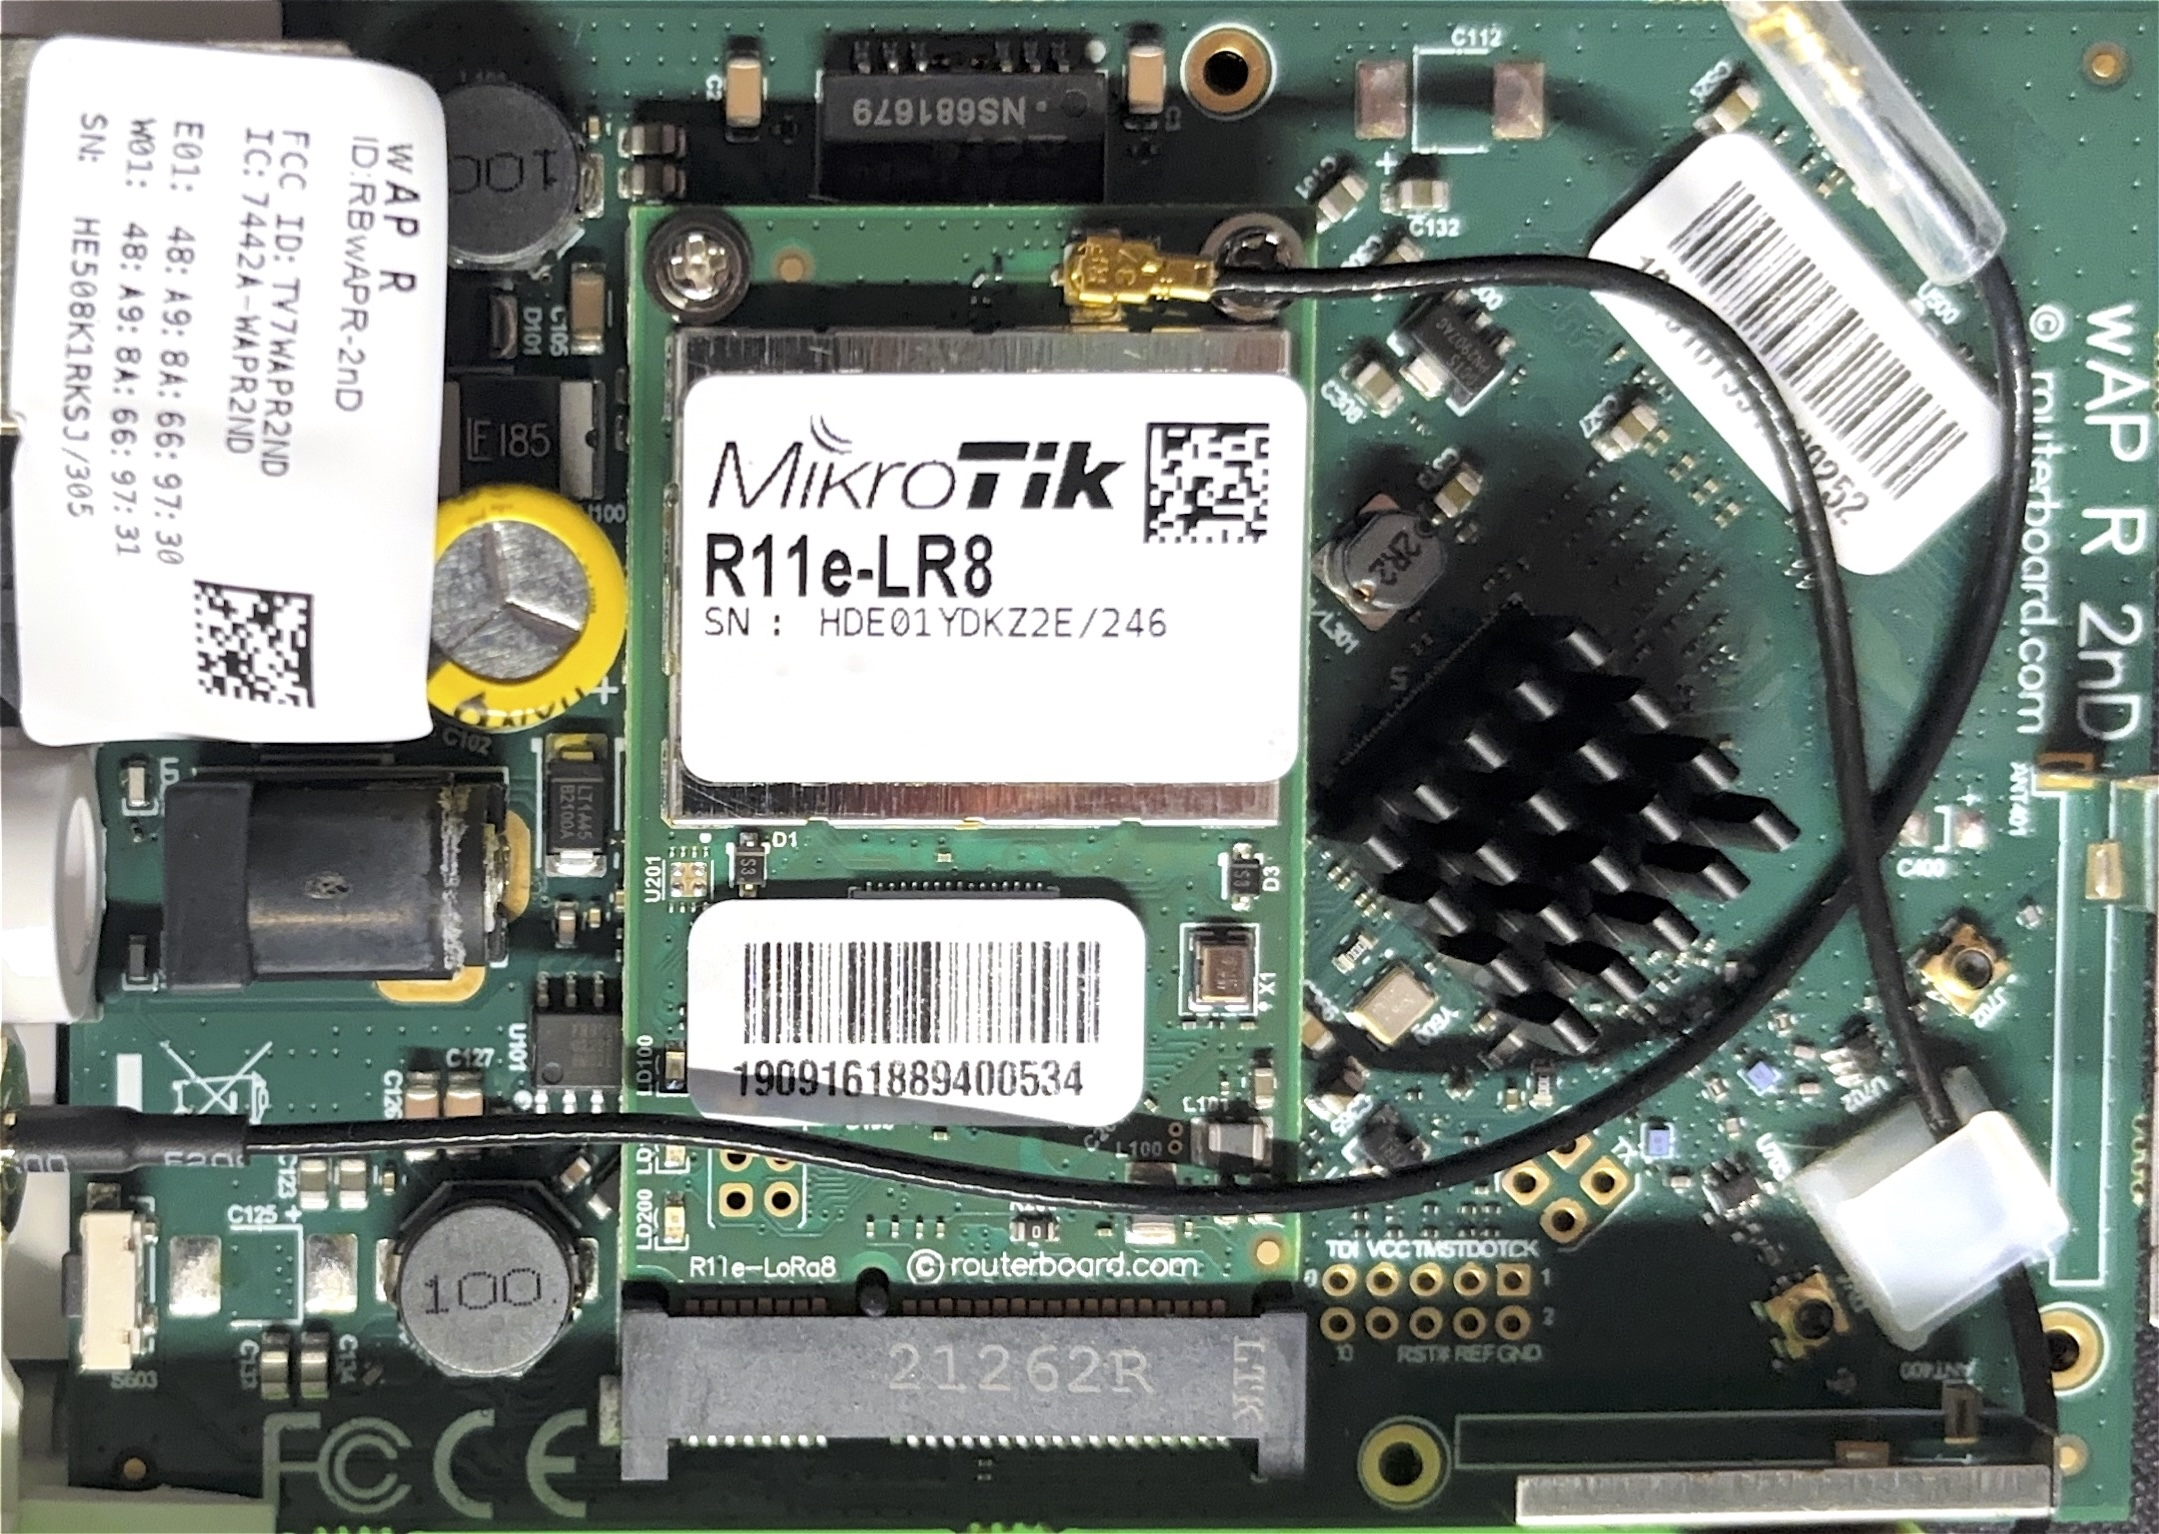
\includegraphics[width=10cm, angle=0]{../Images/LoRaAndLoRaWAN/Gateway/MikrotikCard.jpeg}};
		\end{scope}
	\end{scope}
}


% CARD-UFL-CONNECTOR - coordinate to u.fl
\newcommand{\loraCard}[4]{
	\begin{scope}[shift={(#3, #4)}]
		\tikzset{
			lineScaled/.style n args={1}			{line width={#1*3pt}},
			lineScaledWire/.style n args={1}		{line width={#1*20pt}},
			cornersScaled/.style n args = {1}	    {rounded corners={#1*15pt}},
			cornersScaledSmall/.style n args = {1}	{rounded corners={#1*10pt}},
			cornersScaledBig/.style n args = {1}	{rounded corners={#1*60pt}},
		}
		\begin{scope}[scale=#1, rotate=#2]
			
			\fill[ArduinoColor!80!black] (-2.1, -2.8) rectangle (1, 2.6);
			
			% Antenna connector
			\begin{scope}[shift={(0.1, 2.0)}]
				\begin{scope}[scale=0.3, rotate=0, line width=0.03cm*#1]
					\coordinate (CARD-UFL-CONNECTOR) at (0, 0.9);
					\fill[gray] (-0.6, 0.3) rectangle ++(1.2, 1.2);
					\fill[Gold] (0, 0.9) circle (0.12cm);
					\draw[Gold] (0, 0.9) circle (0.45cm);
				\end{scope}
			\end{scope}
			
			% lora chip
			\fill[gray!50] (-2, -0.3) rectangle (0.9, 2);
			
			% LED
			\begin{scope}[shift={(-1.9, -2.1)}]
				\begin{scope}[rotate=90]
					\foreach \y in {0} {
						\foreach \i in {0,...,2} {
							\pgfmathsetmacro{\x}{\i*0.35}
							\SMDLed{0.08}{90}{\x}{\y}{yellow}
						}
					}
				\end{scope}
			\end{scope}
			
			
			\begin{scope}[shift={(-1.6, -2)}]
				\begin{scope}[rotate=0]
					\foreach \y in {0, 0.2} {
						\foreach \i in {0,...,1} {
							\pgfmathsetmacro{\x}{\i*0.2}
							\draw[Gold, line width=0.35mm*#1] (\x, \y) circle (0.06cm);
						}
					}
				\end{scope}
			\end{scope}
			
			\begin{scope}[shift={(-1.1, -2.15)}]
				\begin{scope}[rotate=0]
					\foreach \y in {0} {
						\foreach \i in {0,...,3} {
							\pgfmathsetmacro{\x}{\i*0.15}
							\smallSMDCapacitor{0.04}{0}{\x}{\y}{ArduinoColor}
						}
					}
				\end{scope}
			\end{scope}
			
			\smallSMDResistor{0.09}{90}{0.7}{-1.7}{ArduinoColor}
			\smallSMDResistor{0.05}{0}{0.9}{-1.5}{ArduinoColor}
			\smallSMDResistor{0.08}{90}{-0.1}{-2.1}{ArduinoColor}
			\smallSMDResistor{0.09}{0}{-0.5}{-2.1}{ArduinoColor}
			
			\fill[gray!30] (0.5, -1.1) rectangle ++(0.3, 0.4);
			
			% dioden
			\begin{scope}[shift={(0.8, -0.5)}]
				\fill[black] (-0.07, -0.1) rectangle (0.07, 0.1);
				\fill[gray] (-0.015, 0.1) rectangle (0.015, 0.13);
				\fill[gray] (-0.015, -0.1) rectangle (0.015, -0.13);
				\fill[gray] (-0.07, 0.065) rectangle (0.07, 0.08);
			\end{scope}
			
			\begin{scope}[shift={(-1.6, -0.45)}]
				\fill[black] (-0.07, -0.1) rectangle (0.07, 0.1);
				\fill[gray] (-0.015, 0.1) rectangle (0.015, 0.13);
				\fill[gray] (-0.015, -0.1) rectangle (0.015, -0.13);
				\fill[gray] (-0.07, 0.065) rectangle (0.07, 0.08);
			\end{scope}
			
			% chip
			\begin{scope}[shift={(-0.5, 0)}]
				\begin{scope}[scale=0.5, rotate=0]
					\fill[black] (-1.1, -3.2) rectangle (0.95, -1.2);
					
					\foreach \x in {-1.1, 0.95} {
						\foreach \i in {0,...,10} {
							\pgfmathsetmacro{\y}{-3.05 + \i*0.17}
							\fill[gray] ({\x-0.08}, {\y-0.05}) rectangle ({\x+0.08}, {\y+0.05});
						}
					}
					
					\foreach \y in {-3.2, -1.2} {
						\foreach \i in {0,...,10} {
							\pgfmathsetmacro{\x}{-0.94 + \i*0.17}
							\fill[gray] ({\x-0.05}, {\y-0.08}) rectangle ({\x+0.05}, {\y+0.08});
						}
					}
				\end{scope}
			\end{scope}
			
			%\fill[red] (-2.1, -2.8) rectangle (1, 2.6);
			% Drills
			\foreach \x/\y in {-1.8/2.35, 0.7/2.35} {
				\fill[white] (\x, \y) circle (1.5mm);
				\draw[Gold, line width=0.9mm*#1] (\x, \y) circle (1.6mm);
			}
			
			% PCIe connector
			\foreach \i in {0,...,7} {
				\pgfmathsetmacro{\y}{-2.8}
				\pgfmathsetmacro{\x}{-1.8 + \i*0.085}
				\fill[Gold] ({\x-0.03}, {\y}) rectangle ({\x+0.03}, {\y+0.25});
			}
			
			\foreach \i in {0,...,17} {
				\pgfmathsetmacro{\y}{-2.8}
				\pgfmathsetmacro{\x}{-0.8 + \i*0.085}
				\fill[Gold] ({\x-0.03}, {\y}) rectangle ({\x+0.03}, {\y+0.25});
			}
			% Background template picture -> edit in scale 1
			%\node[anchor=center, inner sep=0pt, opacity=0.3] at (0,0) {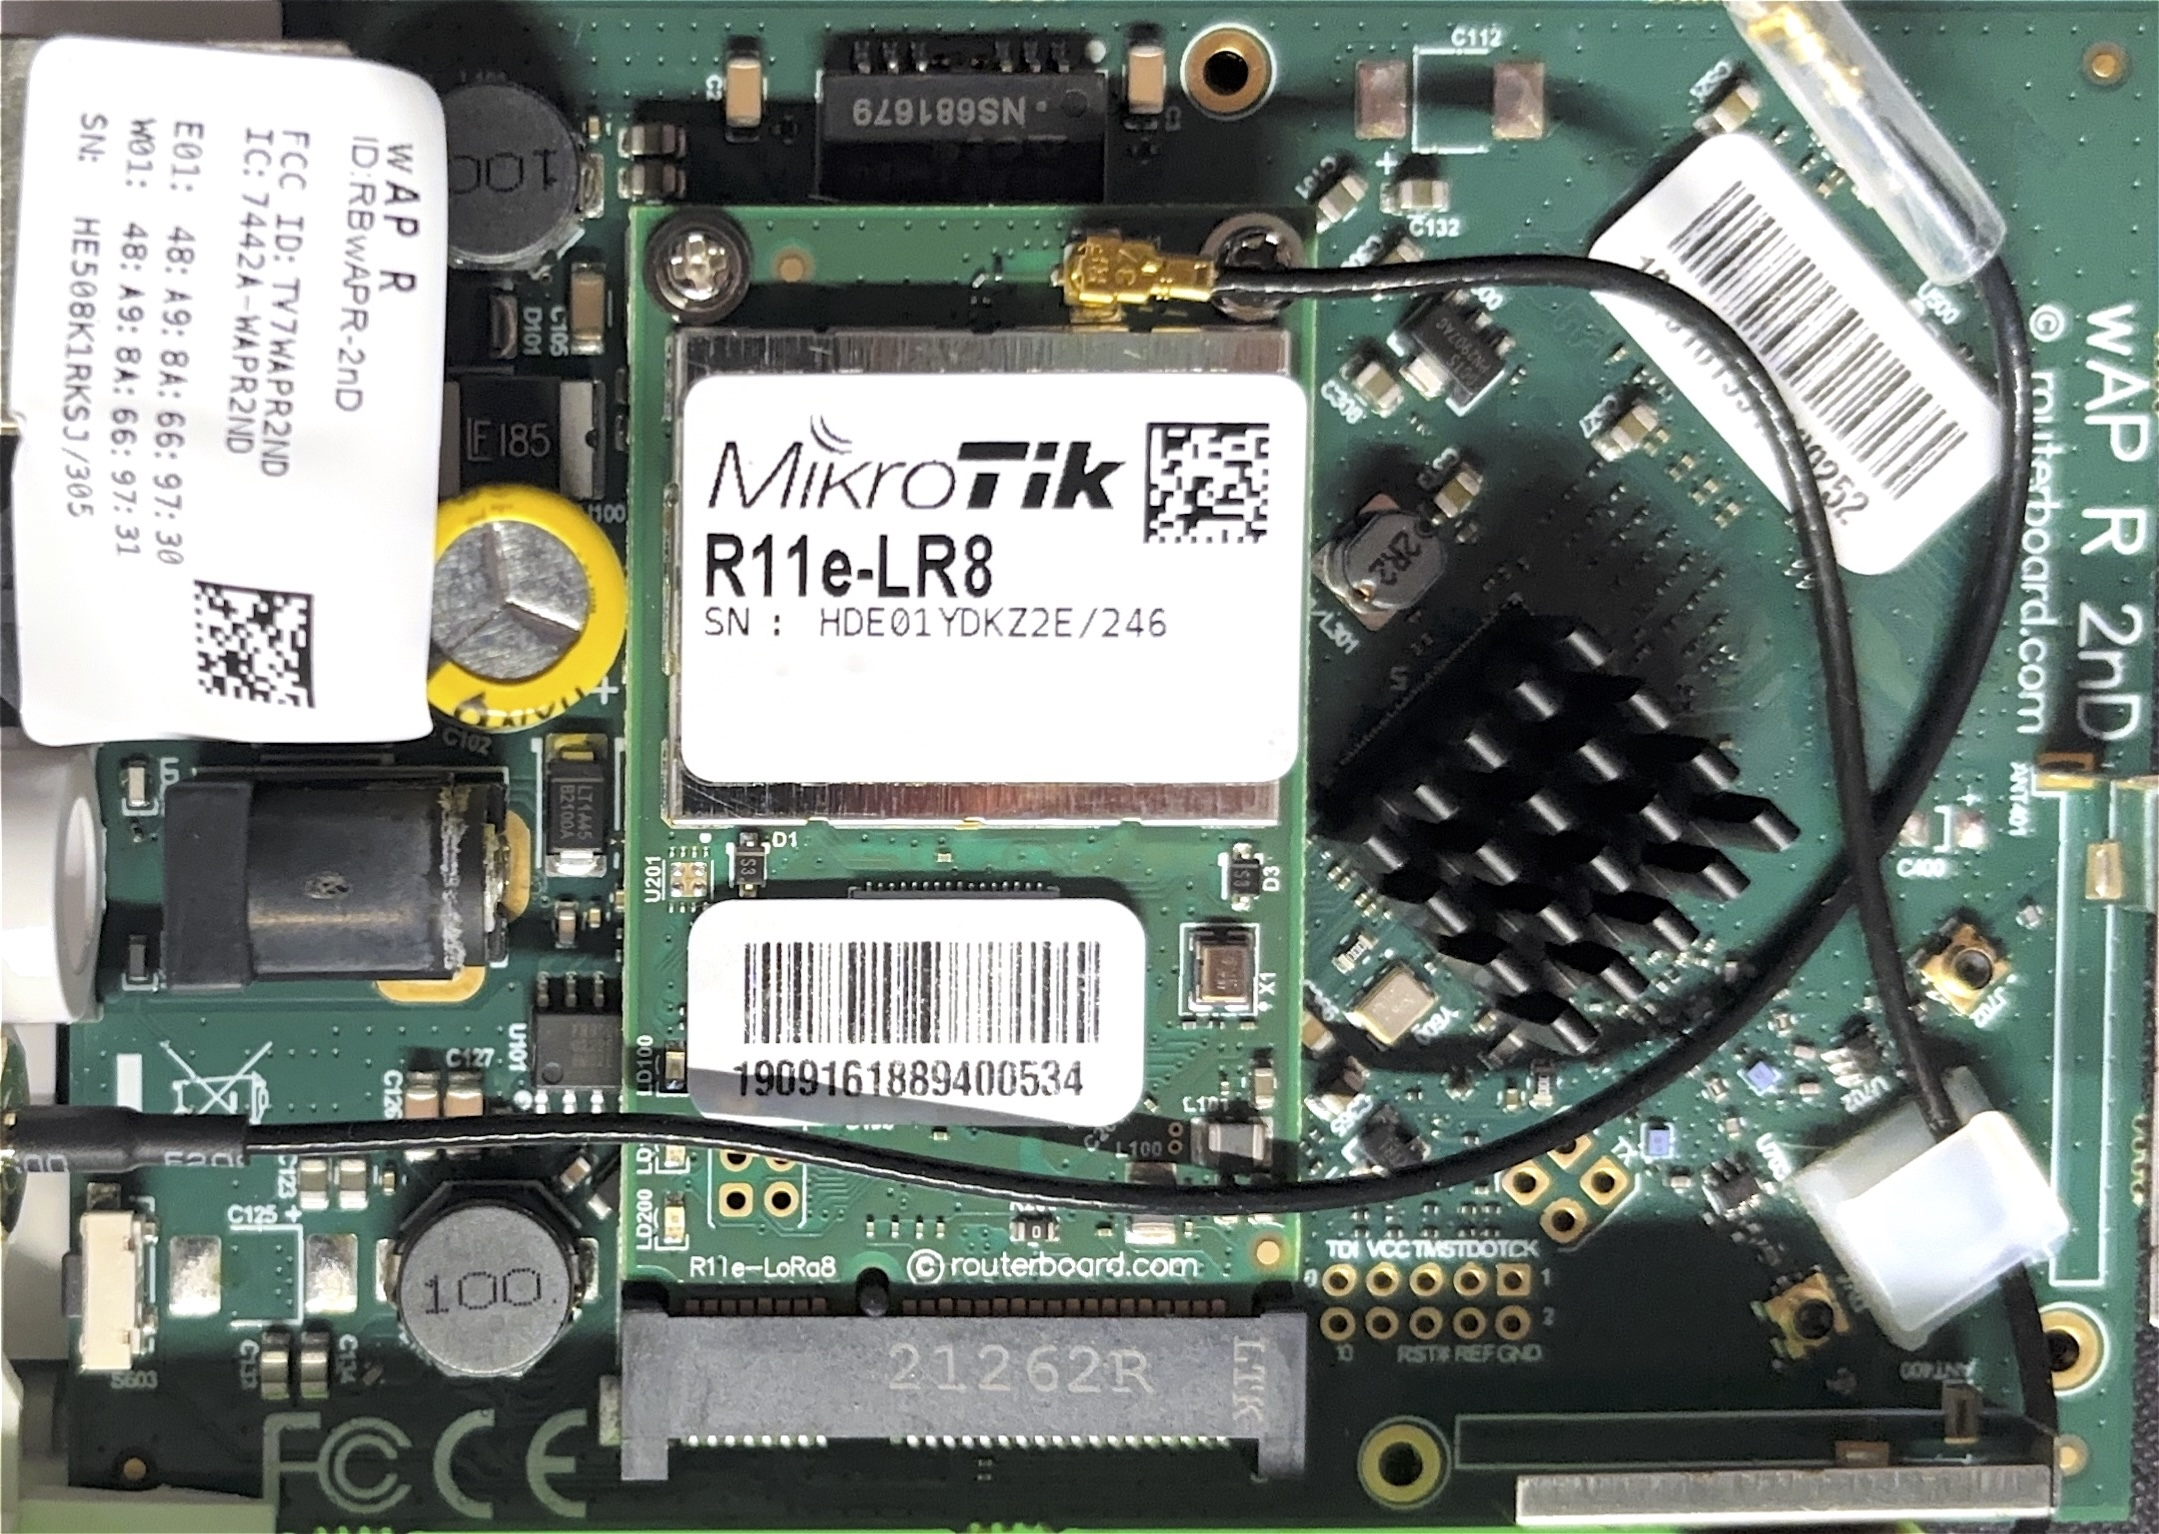
\includegraphics[width=10cm, angle=0]{../Images/LoRaAndLoRaWAN/Gateway/MikrotikCard.jpeg}};
		\end{scope}
	\end{scope}
}




% #1 = scale
% #2 = angle
% #3 = x coordinate
% #4 = y coordinate
% #5 = x length
% #6 = y length
% #7 = pins count oben
% #8 = pins count unten
% #9 = pins width
\newcommand{\SMDTransistorAuto}[9]{
	\begin{scope}[shift={(#3, #4)}]
		\begin{scope}[scale=#1, rotate=#2]
			
			% main body
			\fill[black] ({-#5}, {-#6}) rectangle ({#5}, {#6});
			
			% Compute offset for pin centers
			\pgfmathsetmacro{\offset}{#9/2}
			
			
			% ---------- Upper pins (#7) centered ----------
			\ifnum#7>0
			\pgfmathsetmacro{\offset}{#9}
			\pgfmathsetmacro{\usable}{2*#5 - 2*\offset}
			\pgfmathsetmacro{\halfusable}{\usable/2}
			
			% Generate X positions
			\ifnum#7=1
			\def\XlistA{0} % jedno miejsce - środek
			\else
			\pgfmathsetmacro{\pitch}{\usable / (#7 - 1)}
			% pierwszy element listy:
			\pgfmathsetmacro{\xmin}{-\halfusable}
			\xdef\XlistA{\xmin} % zaczynamy od pierwszego X
			% kolejne elementy:
			\foreach \i in {1,...,\numexpr#7-1\relax} {
				\pgfmathsetmacro{\x}{\xmin + \i*\pitch}
				\xdef\XlistA{\XlistA,\x}
			}
			\fi
			
			% draw pins
			\foreach \x in \XlistA {
				\fill[gray] (\x - #9/2, #6) rectangle (\x + #9/2, #6 + 0.2);
			}
			\fi
			
			
			
			% ---------- Lower pins (#8) centered ----------
			\ifnum#8>0
			\pgfmathsetmacro{\offset}{#9}
			\pgfmathsetmacro{\usable}{2*#5 - 2*\offset}
			\pgfmathsetmacro{\halfusable}{\usable/2}
			
			% Generate X positions
			\ifnum#8=1
			\def\XlistB{0}
			\else
			\pgfmathsetmacro{\pitch}{\usable / (#8 - 1)}
			\pgfmathsetmacro{\xmin}{-\halfusable}
			\xdef\XlistB{\xmin} % pierwszy element
			\foreach \i in {1,...,\numexpr#8-1\relax} {
				\pgfmathsetmacro{\x}{\xmin + \i*\pitch}
				\xdef\XlistB{\XlistB,\x}
			}
			\fi
			
			% draw pins
			\foreach \x in \XlistB {
				\fill[gray] (\x - #9/2, -#6) rectangle (\x + #9/2, -#6 - 0.2);
			}
			\fi
			
			
			
		\end{scope}
	\end{scope}
}


\newcommand{\gatewayConnectors}{
	\tikzset{
		lineScaled/.style={line width={3pt}},
		lineScaledWire/.style={line width={20pt}},
		cornersScaled/.style={rounded corners={15pt}},
		defaulttext/.style={font=\sffamily\scriptsize},
	}
	
	\fill[gray!30] (-5, 1.5)[cornersScaled] -- (-4, -1) -- (4, -1) -- (5, 1.5) -- cycle;
	
	% LAN Port
	\lanPort{0.7}{0}{-2.7}{0.25}
	\node[defaulttext, anchor=north, yshift=-2.3mm] at (-2.7, -0.2) {ETH PoE};
	
	% Molex
	\begin{scope}[shift={(-1.5, -0.4)}]
		\fill[gray!50] (0, 0) rectangle ++(1, 1);
		\fill[gray!50] (0.25, 0.5) rectangle ++(0.5, 0.75);
		
		\foreach \x in {0.3, 0.7} {
			\pgfmathsetmacro{\n}{0.15}
			\foreach \y in {0.3, 0.7} {
				\fill[gray!80] ({\x-\n}, {\y-\n}) rectangle ({\x+\n}, {\y+\n});
				\fill[Gold] (\x, \y) circle (0.5mm);
			}
		}
		
		\draw[line width = 0.4mm] (0, -0.15) -- (1, -0.15);
		\draw[line width = 0.4mm] (0, -0.25) -- (0.25, -0.25);
		\draw[line width = 0.4mm] (0.35, -0.25) -- (0.65, -0.25);
		\draw[line width = 0.4mm] (0.75, -0.25) -- (1, -0.25);
	\end{scope}
	
	\begin{scope}[shift={(0.50, 0.3)}]
		\fill[gray!10] (0, 0) circle (4mm);
		\fill[black] (0, 0) circle (3mm);
		\fill[gray!20] (0, 0) circle (0.5mm);
		
		\node[defaulttext, anchor=south, yshift=3.5mm] at (0, 0) {POWER};
	\end{scope}
	
	\begin{scope}[shift={(1.7, 0.3)}]
		\fill[Gold] (0, 0) circle (4mm);
		\node[fill=Gold!70!black, regular polygon, regular polygon sides=6, minimum size=0.7cm] at (0,0) {};
		\fill[Gold] (0, 0) circle (2.5mm);
		\fill[white] (0, 0) circle (2mm);
		\fill[Gold] (0, 0) circle (0.5mm);
		
		\node[defaulttext, anchor=north, yshift=-3.5mm] at (0, 0) {RF out};
	\end{scope}
	
	\fill[black] (2.9,-0.4) circle (1mm);
	\node[defaulttext, anchor=south, yshift=0.3mm] at (2.9, -0.4) {RESET};
	
}


\newcommand{\lanPort}[4]{
	\begin{scope}[shift={(#3, #4)}]
		\begin{scope}[scale=#1, rotate=#2]	
			\tikzset{
				lineScaled/.style n args={1}			{line width={#1*4pt}},
				cornersScaled/.style n args = {1}	    {rounded corners={#1*8pt}},
			}
			
			
			\fill[gray!50] (-1.2, -1) rectangle (1.2, 1);
			\fill[gray!80] (-1.0, -0.8) rectangle (1.0, 0.6);
			\fill[gray!80] (-0.25, 0.55) rectangle (0.25, 0.8);
			
			\fill[green!70!black] (-0.9, 0.6) rectangle ++(0.5, 0.2);
			\fill[orange!70!black] (0.9, 0.6) rectangle ++(-0.5, 0.2);
			
		\end{scope}
	\end{scope}
}

\newcommand{\uFlConnector}[4]{
	\begin{scope}[shift={(#3, #4)}]
		\begin{scope}[scale=#1, rotate=#2]	
			\tikzset{
				lineScaled/.style n args={1}			{line width={#1*4pt}},
				cornersScaled/.style n args = {1}	    {rounded corners={#1*8pt}},
			}
			
			
			\fill[gray!50] (-1.2, -1) rectangle (1.2, 1);
			\fill[gray!80] (-1.0, -0.8) rectangle (1.0, 0.6);
			\fill[gray!80] (-0.25, 0.55) rectangle (0.25, 0.8);
			
			\fill[green!70!black] (-0.9, 0.6) rectangle ++(0.5, 0.2);
			\fill[orange!70!black] (0.9, 0.6) rectangle ++(-0.5, 0.2);
			
		\end{scope}
	\end{scope}
}

\newcommand{\screwView}{
	\tikzset{
		lineScaled/.style={line width={3pt}},
		cornersScaled/.style={rounded corners={15pt}},
		arrowStyle/.style={line width=2pt, >=stealth, red},
	}
	
	\fill[gray!30] (-5, 1.5)[cornersScaled] -- (-4, -1) -- (4, -1) -- (5, 1.5) -- cycle;
	
	\fill[gray!70] (0, 0) circle (4mm);
	\draw[black, lineScaled] (-0.2, 0) -- (0.2, 0);
	\draw[black, lineScaled] (0, -0.2) -- (0, 0.2);
	
	\draw[->, arrowStyle] (0:7mm) arc (0:180:7mm);
	
}

% #1 = scale
% #2 = angle
% #3 = x coordinate
% #4 = y coordinate
% #5 = Connector Number
% LAN-CONN
\newcommand{\lanConnectorCable}[5]{
	\begin{scope}[shift={(#3, #4)}]
		\begin{scope}[scale=#1, rotate=#2]	
			\tikzset{
				lineScaled/.style n args={1}			{line width={#1*4pt}},
				lineSmall/.style n args={1}			{line width={#1*2pt}},
				cornersScaled/.style n args = {1}	    {rounded corners={#1*8pt}},
				cornersScaledMore/.style n args = {1}	    {rounded corners={#1*6pt}},
			}
			
			
			\fill[gray!50] (-1, -1.3) rectangle (1, 1.3);
			\fill[gray!30] (-0.2, 1.3) rectangle (0.2, 0.6);
			\fill[gray!30] (-0.1, 0.65) rectangle (0.1, -0.3);
			
			%\fill[blue] (-1.15, -1.2) rectangle (1.15, -1.5);
			\fill[blue] (-1.15, -0.9)[cornersScaled] -- (-1.15, -2) -- (1.15, -2)[sharp corners] -- (1.15, -0.9) -- cycle; 
			\fill[blue, cornersScaledMore] (-0.4, -1) rectangle (0.4, -3);
			
			\foreach \i in {0,...,2} {
				\pgfmathsetmacro{\y}{-2.7 + \i*0.27}
				\draw[black, lineSmall] (-0.4, \y) -- ++(0.3, 0);
				\draw[black, lineSmall] (0.4, \y) -- ++(-0.3, 0);
				\draw[black, lineSmall] (-0.15, {\y-0.13}) -- ++(0.3, 0);
			}
			\coordinate(LAN-CONN-#5) at (0, -3);
			
		\end{scope}
	\end{scope}
}
